\part*{附录二：具体构造}
\addcontentsline{toc}{part}{附录二：具体构造}
\chapter{（带标记）单纯集的组合学}\label{ch:marked-simplicial-sets}


在本附录中，我们探究\trSimplicialSet{}的组合学，证明第 1 章与第 4 章中所述的%
诸结果。这些结果当中的某一些——即那些涉及\trQuasiCategory{}中\trIsomorphism{}的%
结果——在与之密切相关的「带标记」\trSimplicialSet{}的\trCategory{}中更容易证明：
在该范畴中，诸\trQuasiCategory{}被等同于那些\emph{$1$-\trComplicial}%
\trMarkedSimplicialSet。由于相应的\emph{$n$-复状\trSimplicialSet}%
（$n$-complicial sets）构成附录 E 中出现的诸\trInfinityCosmos{}的例子族之一，
我们便在那一更一般的语境中证明必要的组合结果。

\trMarkedSimplicialSet{}的\trCategory{}将在 D.1 节中引入。该\trCategory{}中某些在%
一切维数下都具有诸\trSimplex{}之复合的对象，定义了\emph{复状\trSimplicialSet}%
（complicial sets）——它们由一种右\trLifting{}性质所刻画，而这一性质同样%
定义了\emph{复状\trIsofibration}（complicial isofibrations）。在 D.2 节中，我们%
通过重访 4.2 节中的\trJoin{}与切片构造来开始组合学的工作，并从\trAugmented{}%
\trSimplicialSet{}的视角出发重新发展这些概念。这一工作在 D.6 节中完成，我们在%
其中证明：一个\trDiagram{}之上或之下的\trCone{}的\trQuasiCategory{}的各种模型%
相互等价。

在 D.3 节中，我们证明复状\trIsofibration{}在以\trMarkedSimplicialSet{}的%
\trMonomorphism{}作幂之下的 Leibniz 稳定性。这一点与 1.1 节中若干未加证明的%
结果颇为相似，但在建立这一联系之前，我们必须先把复状\trSimplicialSet{}与%
复状\trIsofibration{}同\trQuasiCategory{}与\trIsofibration{}关联起来。这一任务%
占据了余下的两节。在 D.4 节中，我们建立复状\trSimplicialSet{}理论与%
\trQuasiCategory{}理论之间的联系，证明任何\trQuasiCategory{}都可以配备一个%
以\trCanonical{}方式定义的「自然」标记，使得它定义一个凡维数大于 $1$ 的\trSimplex{}皆被%
标记的复状\trSimplicialSet。其证明需要仔细研究定义\trQuasiCategory{}中%
\trIsomorphism{}的那些数据。在 D.5 节中应用这一分析，我们证明 Joyal 的%
「特殊外\trHorn{}填充」命题（第 1 章中的%
\cref{prop:special-outer-horn-filling}），它无非是下述观察：自然标记%
\trQuasiCategory{}之间的\trIsofibration{}与复状\trIsofibration{}恰好重合。%
这一联系一经建立，前述诸结果便可以汇集起来，为 1.1 节中的诸论断提供证明。



\section{复状单纯集}\label{sec:complicial-sets}

当把一个\trQuasiCategory{}视为一个 $(\infty,1)$-范畴时，其顶点扮演对象的
角色，其边表示态射，而顶点处的退化边则表示其恒同。诸 $n$-\trSimplex{}于是见证
$n$ 元复合关系。而当把一个\textbf{复状单纯集}（complicial set）视为一个
$(\infty,\infty)$-范畴时，其诸 $n$-\trSimplex{}必须扮演一个双重角色：既充当较低
维复合关系的见证者，而本身又代表先验不可逆的 $n$ 维胞腔。为区分这
两种诠释，复状单纯集中某些正维数的\trSimplex{}被\emph{标记}为「薄的」，表明它们
应被诠释为其\trBoundary{}诸面之间弱复合关系的\trEquivalence{}见证。于是，
定义复状单纯集所用的周围\trCategory{}并非通常\trSimplicialSet{}的%
\trCategory，而是一个密切相关的\textbf{%
\trMarkedSimplicialSet}（marked simplicial set）范畴，我们现在就来引入它。%
\footnote{在原始文献 \cite{bib128,bib129} 中，\trMarkedSimplicialSet{}称作\emph{分层%
\trSimplicialSet{}}（stratified simplicial sets）。为免与日渐盛行的另一个互不相干的
分层空间（stratified spaces）概念相混淆，我们决意改名。在 \cite{bib78} 中，
Lurie 将\emph{\trMarkedSimplicialSet{}}（marked simplicial sets）一词用于我们即将引入
的更一般概念的一个特例。}

\begin{definition}[\trMarkedSimplicialSet{}]\label{def:marked-simplicial-sets}
一个\textbf{\trMarkedSimplicialSet}是一个\trSimplicialSet，连同由\textbf{%
带标记}或\textbf{薄}（thin）的正维数\trSimplex{}组成的一个指定子集，该子集包含
一切退化\trSimplex{}。\trMarkedSimplicialSet{}之间的一个映射，是一个保持带标记\trSimplex{}的单纯
映射。
\end{definition}

\begin{definition}[极小标记与极大标记]\label{def:minimal-maximal-marking}
\trMarkedSimplicialSet{}的\trCategory{} $\sSet^{+}$ 配备一个通往 $\sSet$ 的明显%
\trForgetfulFunctor{}，后者兼有\trLeftAdjoint{}与\trRightAdjoint：
\begin{center}
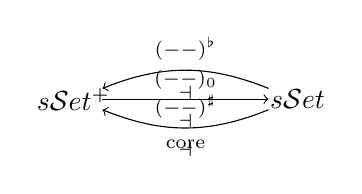
\begin{tikzpicture}[x=1.5em,y=1.1em]
  \node (L) at (0,0) {$\sSet^{+}$};
  \node (R) at (5.4,0) {$\sSet$};
  \draw[->] (4.7,0.35) to[bend right=22] node[pos=0.5,above]{$\scriptstyle(\text{--})^{\flat}$} node[pos=0.5,below=2pt]{$\scriptstyle\dashv$} (0.7,0.35);
  \draw[->] (0.7,0) -- node[pos=0.5,above]{$\scriptstyle(\text{--})_{0}$} node[pos=0.5,below=2pt]{$\scriptstyle\dashv$} (4.7,0);
  \draw[->] (4.7,-0.35) to[bend left=22] node[pos=0.5,above]{$\scriptstyle(\text{--})^{\sharp}$} node[pos=0.5,below=2pt]{$\scriptstyle\dashv$} (0.7,-0.35);
  \node at (2.7,-1.5) {$\scriptstyle\mathrm{core}$};
\end{tikzpicture}
\end{center}
\end{definition}

\trLeftAdjoint{} $(-)^{\flat}$ 给出\trSimplicialSet{}的\textbf{极小标记}（minimal
marking），其中只有退化\trSimplex{}被标记；\trRightAdjoint{} $(-)^{\sharp}$ 给出
\textbf{极大标记}（maximal marking），一切\trSimplex{}都被标记。这一函子还有一个
更进一层的\trRightAdjoint，它把一个\trMarkedSimplicialSet{}送到其\textbf{核}（core）：
即一个\trSimplicialSet{}，与原来具有相同的顶点，由那些诸面同样被标记的带标记\trSimplex{}所
组成。

在多种场合下，把 $\sSet$ 与刚刚引入的两支通往 $\sSet^{+}$ 的全忠实嵌入中的
某一者相认同是便利的。除非另有指明，默认约定是把\trSimplicialSet{}与其极小标记相
认同。特别地，在此约定下，我们可以自由地把标准\trSimplex{}及其子空间视为极小
标记的\trMarkedSimplicialSet{}。

为简便地引入其他\trMarkedSimplicialSet{}，下述术语是便利的：

\begin{definition}\label{def:regular-entire-inclusions}
\trMarkedSimplicialSet{}之间的一个包含 $U\hookrightarrow V$ 是：
\begin{itemize}
\item \textbf{正则的}（regular），记作 $U\hookrightarrow_{r}V$，若 $U$ 中的
  薄\trSimplex{}在 $V$ 中被创造；
\item \textbf{整的}（entire），记作 $U\hookrightarrow_{e}V$，若该映射在底%
  \trSimplicialSet{}上是\trIsomorphism（或更常见地，是恒同），此时 $U$ 与
  $V$ 之间的唯一差别在于 $V$ 带有更多的带标记\trSimplex{}。
\end{itemize}
\end{definition}

例如，对每个 $n\ge 1$，我们把\textbf{带标记\trSimplex}（marked simplex）
$\Delta[n]_{t}$ 定义为极小标记\trSimplex{} $\Delta[n]$ 的整扩张，后者还标记
最高维非退化\trSimplex{}。

\begin{notation}[带标记\trSimplex{}范畴]\label{not:marked-simplex-category}
设 $t\Delta\hookrightarrow\sSet^{+}$ 表示由极小标记\trSimplex{} $\Delta[n]$
（$n\ge 0$）连同带标记\trSimplex{} $\Delta[n]_{t}$（$n\ge 1$）所张成的全子范畴。
它可由第 1 章中的\cref{not:simplex-category} 的\trSimplex{}范畴 $\Delta$ 构建
如下：
\begin{itemize}
\item 添入对象 $[n]_{t}$，对 $n\ge 1$；
\item 添入映射 $\phi\colon[n]\to[n]_{t}$，对 $n\ge 1$；以及
  $\xi^{i}\colon[n+1]_{t}\to[n]$，对 $n\ge 0$ 与 $0\le i\le n$；并且
\item 强加关系 $\xi^{i}\phi=\sigma^{i}$ 与%
  $\sigma^{i}\xi^{j+1}=\sigma^{j}\xi^{i}$，对 $i\le j$。\footnote{Viktoriya Ozornova 与 Martina
  Rovelli 向我们指出：最后这一族关系在原始文献 \cite{bib122} 中被遗漏了，
  但本应包含在内。一个修正后的定义见 \cite[1.1]{bib89}。}
\end{itemize}
\end{notation}

对一个\trMarkedSimplicialSet{} $X$，映射 $\Delta[n]\to X$ 与 $\Delta[n]_{t}\to X$ 分别
参数化 $X$ 中的 $n$-\trSimplex{}与 $X$ 中的带标记 $n$-\trSimplex{}。这定义了一个\trCanonical{}%
嵌入 $\sSet^{+}\hookrightarrow\mathcal{S}et^{t\Delta^{\mathrm{op}}}$，容易
看出它是\trFullyFaithful。此外：

\begin{proposition}\label{prop:reflective-embedding}
存在一个反射嵌入（reflective embedding）
\begin{center}
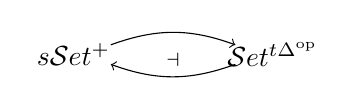
\begin{tikzpicture}[x=1.5em,y=1.1em]
  \node (L) at (0,0) {$\sSet^{+}$};
  \node (R) at (4.8,0) {$\mathcal{S}et^{t\Delta^{\mathrm{op}}}$};
  \draw[->] (0.9,0.32) to[bend left=20] (3.9,0.32);
  \draw[->] (3.9,-0.32) to[bend left=20] node[pos=0.5,above]{$\scriptstyle\dashv$} (0.9,-0.32);
\end{tikzpicture}
\end{center}
其
\begin{enumerate}[label=(\roman*)]
\item 本质像由那些预层（presheaf）$F$ 组成：其分量映射
  $-\circ\phi\colon F_{[n]_{t}}\to F_{[n]}$ 都是\trMonomorphism；并且
\item 左伴随构造为：把集合 $F_{[n]_{t}}$ 替换为映射
  $-\circ\phi\colon F_{[n]_{t}}\to F_{[n]}$ 的像。
\end{enumerate}
\end{proposition}

\emph{从而，$\sSet^{+}$ 是一个局部有限可表现（locally finitely
presentable）的范畴，特别地是完备且余完备的：其诸\trLimit{}作为预层逐点
构造，而其诸\trColimit{}则通过把反射作用施加于预层的逐点余极限而构造。}

{\tolerance=3000\emergencystretch=3em%
用更初等的话来说：\trMarkedSimplicialSet{}的诸\trLimit{}与诸\trColimit{}由底%
\trSimplicialSet{}函子 $(-)_{0}\colon\sSet^{+}\to\sSet$ 所创造。\trLimit{}%
中的一个\trSimplex{}被标记，当且仅当它的\emph{每一个}分量——通过沿\trLimit{}
\trCone{}的诸腿作复合而定义——都是带标记\trSimplex{}。\trColimit{}中的一个\trSimplex{}%
被标记，若它沿余极限锥的任一条腿的\emph{任一}\trLifting{}是带标记\trSimplex{}。(ii) 中
的反射是一种「命题截断」（propositional truncation）：它记住哪些\trSimplex{}应当
被标记，而忘掉指示其缘由的数据。\par}

\begin{proof}
$t\Delta$ 中诸算子在一个预层 $F\in\mathcal{S}et^{t\Delta^{\mathrm{op}}}$ 上的
右作用，赋予 $F$ 的诸元素之集一个\trMarkedSimplicialSet{}的结构，唯一的例外是一个条件：
即带标记 $n$-\trSimplex{}构成 $n$-\trSimplex{}的一个子集。这解释了出现于 (i) 中的条件
与出现于 (ii) 中的构造。由此可知：\trMarkedSimplicialSet{}乃是一个有限极限草图
（finite limit sketch）之诸模型的\trCategory，从而构成一个局部有限可表现的%
\trCategory。完备且余完备的\trCategory{}的任何反射全子范畴，都按陈述中所
构造的方式继承极限（例如见 \cite[4.5.15]{bib104}）。
\end{proof}

附录 C 中的\cref{lem:mono-epi-reedy-sset}可以推广到\trMarkedSimplicialSet{}的情形，
如下：

\begin{lemma}\label{lem:mono-marked-cellularly-generated}
$\sSet^{+}$ 中的诸\trMonomorphism{}由
\[
\{\partial\Delta[n]\hookrightarrow_{r}\Delta[n]\}_{n\ge 0}
\;\cup\;
\{\Delta[n]\hookrightarrow_{e}\Delta[n]_{t}\}_{n\ge 1}
\]
\trCell{}式生成。
\end{lemma}

\begin{proof}
见\cref{ex:prove-lem-mono-generated}。
\end{proof}

一个\trMarkedSimplicialSet{}是一个带有足够结构的\trSimplicialSet{}，使我们得以谈论所有维数上\trSimplex{}%
的复合。一个复状单纯集是一个\trMarkedSimplicialSet{}，其中复合存在，而且复合的诸薄见证
者相复合而定义薄\trSimplex{}——这一结合性条件最终蕴含：薄\trSimplex{}是某种意义下的%
\trEquivalence，其确切含义在\cref{lem:marked-edges-equivalences}与%
\cref{dig:saturation-higher-simplices}中给出。下述这一
形式的复状单纯集定义（旧称\emph{弱}复状单纯集）归于 \trVerity{} \cite{bib129}，它
修改了早先归于 Street \cite{bib120} 的一个等价表述。\trVerity{}的修改聚焦
于一类特别的\emph{$k$-容许 $n$-\trSimplex{}}：它们是把自己的第 $k$ 面展现为
第 $(k+1)$ 面与第 $(k-1)$ 面之复合的薄 $n$-\trSimplex{}——在 $0<k<n$ 的情形。

而当 $k=0$ 或 $k=n$ 时，一个 $k$-容许 $n$-\trSimplex{}分别见证最初一对面之间或
最后一对面之间的\trEquivalence。

\begin{definition}[$k$-容许 $n$-\trSimplex{}]\label{def:k-admissible-simplex}
对 $n\ge 1$ 与 $0\le k\le n$，\textbf{$k$-容许 $n$-\trSimplex{}} $\Delta^{k}[n]$
是标准 $n$-\trSimplex{}的整超集，其中某些附加的面被标记为薄：$\Delta^{k}[n]$ 中
的一个非退化 $m$-\trSimplex{}是薄的，当且仅当它包含 $\{k-1,k,k+1\}\cap[n]$ 中的
全部顶点。薄面特别包括：
\begin{itemize}
\item 最高维的 $n$-\trSimplex{}；
\item 除第 $(k-1)$ 个、第 $k$ 个与第 $(k+1)$ 个面之外的一切余维一面；
\item 当 $0<k<n$ 时由 $\{k-1,k,k+1\}$ 张成的 2-\trSimplex{}，\yizhu{原书于此印作
  「when $0\le k\le n$」，然 $k=0$ 或 $k=n$ 时并无由 $\{k-1,k,k+1\}$ 张成的
  2-\trSimplex{}（该集含越界顶点），按文义疑为 $0<k<n$ 之误，此处径改。——译者注}或当 $k=0$ 或 $k=n$ 时由 $\{k-1,k,k+1\}\cap[n]$ 张成的边。
\end{itemize}
\end{definition}

在画\trMarkedSimplicialSet{}的图时，我们用符号「$\simeq$」装饰带标记\trSimplex{}，用
「$\sim$」装饰带标记的边。我们的图还采用一个约定，规定栖居于一个无标记
$n$-\trSimplex{}中的胞腔的方向。遵循 Street 在其「定向\trSimplex{}之代数」\cite{bib120}
中引入的组合学，我们把一个 $n$-\trSimplex{}视为一个 $n$-胞腔，从其诸奇数号面的
粘贴复合指向其诸偶数号面的粘贴复合。注意这与既已通用的约定相容，即把\trSimplicialSet{}%
中的一个 1-\trSimplex{}描绘成一支从其第 1 面（第 0 个顶点）指向其第 0 面（第 1 个
顶点）的箭头。

\begin{example}[低维容许\trSimplex{}]\label{exa:admissible-low-dimensions}
\begin{enumerate}[label=(\roman*)]
\item 对 $n=1$，两个容许\trSimplex{} $\Delta^{0}[1]$ 与 $\Delta^{1}[1]$ 都等于薄
  1-\trSimplex{} $\Delta[1]_{t}=\Delta[1]^{\sharp}$。一个映射
  $\Delta[1]^{\sharp}\to A$ 被诠释为在其像中定义两个顶点之间的一个%
  \trEquivalence。
\item 对 $n=2$，容许\trSimplex{} $\Delta^{1}[2]$ 等于薄 2-\trSimplex{} $\Delta[2]_{t}$。
  一个映射 $\Delta^{1}[2]\to A$ 被诠释为指明：$\{02\}$-边的像是 $\{01\}$-边
  与 $\{12\}$-边之像的一个复合。相比之下，$\Delta^{0}[2]$ 与 $\Delta^{2}[2]$
  各有一条带标记的边，也有一个带标记的 2-\trSimplex{}，如下图所示：
\begin{center}
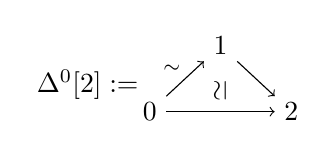
\begin{tikzpicture}[x=1.6em,y=1.4em]
  \node at (-1.4,0.7) {$\Delta^{0}[2]:=$};
  \node (v0) at (0,0) {$0$};
  \node (v1) at (1.6,1.7) {$1$};
  \node (v2) at (3.2,0) {$2$};
  \draw[->] (v0) -- (v1);
  \node at (0.5,1.1) {$\scriptstyle\sim$};
  \draw[->] (v1) -- (v2);
  \draw[->] (v0) -- (v2);
  \node[rotate=90] at (1.6,0.55) {$\simeq$};
\end{tikzpicture}
\qquad
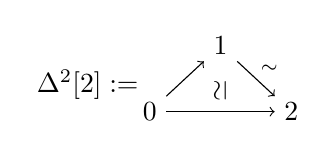
\begin{tikzpicture}[x=1.6em,y=1.4em]
  \node at (-1.4,0.7) {$\Delta^{2}[2]:=$};
  \node (v0) at (0,0) {$0$};
  \node (v1) at (1.6,1.7) {$1$};
  \node (v2) at (3.2,0) {$2$};
  \draw[->] (v0) -- (v1);
  \draw[->] (v1) -- (v2);
  \node at (2.7,1.1) {$\scriptstyle\sim$};
  \draw[->] (v0) -- (v2);
  \node[rotate=90] at (1.6,0.55) {$\simeq$};
\end{tikzpicture}
\end{center}
  一个映射 $\Delta^{0}[2]\to A$ 见证 $\{12\}$-边之像与 $\{02\}$-边之像之间
  的一个\trEquivalence。
\item 对 $n=3$，容许\trSimplex{} $\Delta^{1}[3]$ 与 $\Delta^{2}[3]$ 分别有它们的
  第 3 面与第 0 面被标记，连同最高维的 3-\trSimplex{}，而无任何其他非退化面被
  标记。我们选择以一种能让我们看见全部余维一面的方式来画容许 3-\trSimplex{}：
\begin{center}
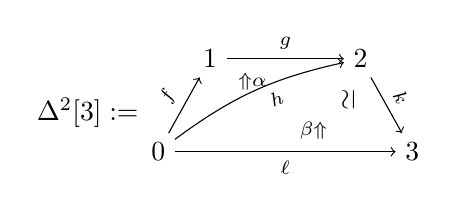
\begin{tikzpicture}[x=1.7em,y=1.4em]
  \node at (-1.5,1.0) {$\Delta^{2}[3]:=$};
  \node (v0) at (0,0) {$0$};
  \node (v3) at (5.4,0) {$3$};
  \node (v1) at (1.1,2.4) {$1$};
  \node (v2) at (4.3,2.4) {$2$};
  \draw[->] (v0) -- node[above,sloped]{$\scriptstyle f$} (v1);
  \draw[->] (v1) -- node[above]{$\scriptstyle g$} (v2);
  \draw[->] (v2) -- node[above,sloped]{$\scriptstyle k$} (v3);
  \draw[->] (v0) to[bend left=12] node[below,sloped,pos=0.6]{$\scriptstyle h$} (v2);
  \draw[->] (v0) -- node[below]{$\scriptstyle\ell$} (v3);
  \node[rotate=90] at (4.05,1.35) {$\simeq$};
  \node at (2.0,1.8) {$\scriptstyle\Uparrow\alpha$};
  \node at (3.3,0.55) {$\scriptstyle\beta\Uparrow$};
\end{tikzpicture}
\quad$\simeq$\quad
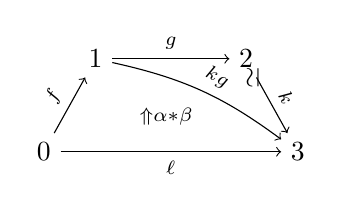
\begin{tikzpicture}[x=1.7em,y=1.4em]
  \node (v0) at (0,0) {$0$};
  \node (v3) at (5.4,0) {$3$};
  \node (v1) at (1.1,2.4) {$1$};
  \node (v2) at (4.3,2.4) {$2$};
  \draw[->] (v0) -- node[above,sloped]{$\scriptstyle f$} (v1);
  \draw[->] (v1) -- node[above]{$\scriptstyle g$} (v2);
  \draw[->] (v2) -- node[above,sloped]{$\scriptstyle k$} (v3);
  \draw[->] (v1) to[bend left=12] node[above,sloped,pos=0.55]{$\scriptstyle kg$} (v3);
  \draw[->] (v0) -- node[below]{$\scriptstyle\ell$} (v3);
  \node[rotate=90] at (4.45,1.9) {$\simeq$};
  \node at (2.6,0.9) {$\scriptstyle\Uparrow\alpha\ast\beta$};
\end{tikzpicture}
\end{center}
  这里我们对诸面加以标号，以便更好地描述一个映射 $\Delta^{2}[3]\to A$ 的
  诠释。它的第 0 面——其自身是一个容许\trSimplex{} $\Delta^{1}[2]$——见证边
  $\{13\}$ 是边 $\{12\}$ 与 $\{23\}$ 的一个复合。注意由于第 0 面是薄的，
  其第 1 边被诠释为 $g$ 与 $k$ 的复合 $kg$；出现于第 2 面中的 2-胞腔之
  边缘要与 $\beta$ 和 $\alpha$ 的粘贴复合之边缘相一致，正需要这一点。鉴于
  这一边缘条件以及薄的 3-\trSimplex{}，我们把第 2 面诠释为右图所描绘的第 1 面与
  第 3 面的粘贴复合。

  容许\trSimplex{} $\Delta^{0}[3]$ 有它的第 2 面与第 3 面被标记，连同最高维的
  3-\trSimplex{}，以及边 $\{01\}$。对偶地，$\Delta^{3}[3]$ 有它的第 0 面与第 1 面
  被标记，连同最高维的 3-\trSimplex{}，以及边 $\{23\}$。
\begin{center}
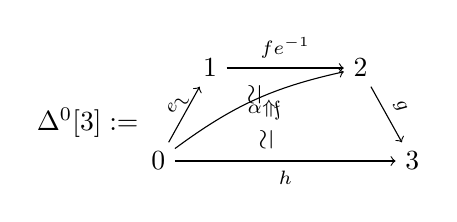
\begin{tikzpicture}[x=1.7em,y=1.4em]
  \node at (-1.5,1.0) {$\Delta^{0}[3]:=$};
  \node (v0) at (0,0) {$0$};
  \node (v3) at (5.4,0) {$3$};
  \node (v1) at (1.1,2.4) {$1$};
  \node (v2) at (4.3,2.4) {$2$};
  \draw[->] (v0) -- node[above,sloped]{$\scriptstyle e$} (v1);
  \node at (0.5,1.5) {$\scriptstyle\sim$};
  \draw[->] (v1) -- node[above]{$\scriptstyle fe^{-1}$} (v2);
  \draw[->] (v2) -- node[above,sloped]{$\scriptstyle g$} (v3);
  \draw[->] (v0) to[bend left=12] node[below,sloped,pos=0.6]{$\scriptstyle f$} (v2);
  \draw[->] (v0) -- node[below]{$\scriptstyle h$} (v3);
  \node[rotate=90] at (2.05,1.7) {$\simeq$};
  \node[rotate=90] at (2.3,0.55) {$\simeq$};
  \node at (2.2,1.35) {$\scriptstyle\alpha\Uparrow$};
\end{tikzpicture}
\quad$\simeq$\quad
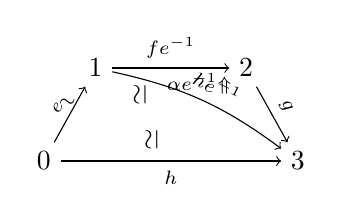
\begin{tikzpicture}[x=1.7em,y=1.4em]
  \node (v0) at (0,0) {$0$};
  \node (v3) at (5.4,0) {$3$};
  \node (v1) at (1.1,2.4) {$1$};
  \node (v2) at (4.3,2.4) {$2$};
  \draw[->] (v0) -- node[above,sloped]{$\scriptstyle e$} (v1);
  \node at (0.5,1.5) {$\scriptstyle\sim$};
  \draw[->] (v1) -- node[above]{$\scriptstyle fe^{-1}$} (v2);
  \draw[->] (v2) -- node[above,sloped]{$\scriptstyle g$} (v3);
  \draw[->] (v1) to[bend left=12] node[above,sloped,pos=0.55]{$\scriptstyle he^{-1}$} (v3);
  \node at (3.3,2.0) {$\scriptstyle\alpha e^{-1}\Uparrow$};
  \draw[->] (v0) -- node[below]{$\scriptstyle h$} (v3);
  \node[rotate=90] at (2.05,1.7) {$\simeq$};
  \node[rotate=90] at (2.3,0.55) {$\simeq$};
\end{tikzpicture}
\end{center}
  一个映射 $\Delta^{0}[3]\to A$ 被诠释为见证分别占据第 0 面与第 1 面的那对
  非薄 2-\trSimplex{}之间的一个\trEquivalence。
\end{enumerate}
\end{example}

\begin{definition}\label{def:complicial-set}
一个\textbf{复状单纯集}是一个\trMarkedSimplicialSet{} $A$：对由以下两族映射给出的%
\textbf{初等带标记\trAnodyneExtension}（elementary marked anodyne extensions），它都
容有\trExtension。
\begin{enumerate}[label=(\roman*)]
\item \textbf{复状号角扩张}（complicial horn extensions）
\begin{rveq}\label{eq:complicial-horn-extension}
\begin{tikzpicture}[x=1.6em,y=1.4em]
  \node (lt) at (0,1.2) {$\Lambda^{k}[n]$};
  \node (rt) at (2.8,1.2) {$A$};
  \node (lb) at (0,-1.2) {$\Delta^{k}[n]$};
  \draw[->] (lt) -- (rt);
  \draw[right hook->] (lb) -- (lt);
  \node at (-0.45,0) {$\scriptstyle r$};
  \draw[->,dashed] (0.45,-1.0) -- (2.35,1.0);
\end{tikzpicture}
\qquad \text{对\quad $n\ge 1$，\ $0\le k\le n$}%
\end{rveq}
是诸\textbf{$k$-容许 $n$-号角}的正则包含。一个内容许 $n$-号角参数化一对
$(n-1)$-\trSimplex{}的「容许复合」。该\trExtension{}定义了一个复合的 $(n-1)$-\trSimplex{}，连同一个薄的 $n$-\trSimplex{}见证者。
\item \textbf{复状薄性扩张}（complicial thinness extensions）
\begin{rveq}\label{eq:complicial-thinness-extension}
\begin{tikzpicture}[x=1.6em,y=1.4em]
  \node (lt) at (0,1.2) {$\Delta^{k}[n]'$};
  \node (rt) at (2.8,1.2) {$A$};
  \node (lb) at (0,-1.2) {$\Delta^{k}[n]''$};
  \draw[->] (lt) -- (rt);
  \draw[right hook->] (lb) -- (lt);
  \draw[->,dashed] (0.45,-1.0) -- (2.35,1.0);
\end{tikzpicture}
\qquad \text{对\quad $n\ge 2$，\ $0\le k\le n$}%
\end{rveq}
是 $\Delta^{k}[n]$ 的两个整超集之间的\trEntireInclusion。\trMarkedSimplicialSet{} $\Delta^{k}[n]'$
由 $\Delta^{k}[n]$ 再标记第 $(k-1)$ 面与第 $(k+1)$ 面而得，而
$\Delta^{k}[n]''$ 则标记了全部余维一面。这一\trExtension{}问题要求：但凡
容许号角中的可复合\trSimplex{}对是薄的，任何复合便也是薄的。
\end{enumerate}
\end{definition}

\begin{example}[复状号角扩张]\label{exa:complicial-horn-extensions}
对 $\Lambda^{2}[4]\hookrightarrow_{r}\Delta^{2}[4]$ 而言，号角中的诸非薄
余维一面给出左图所示的两个具有公共面的 3-\trSimplex{}，而它们的复合则是右图所示的
一个 3-\trSimplex{}。
\begin{center}
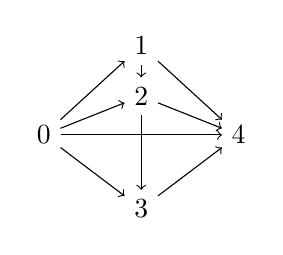
\begin{tikzpicture}[x=1.6em,y=1.4em]
  \node (v1) at (2.2,3.2) {$1$};
  \node (v2) at (2.2,1.9) {$2$};
  \node (v0) at (0,0.9) {$0$};
  \node (v4) at (4.4,0.9) {$4$};
  \node (v3) at (2.2,-1.0) {$3$};
  \draw[->] (v0) -- (v1);
  \draw[->] (v1) -- (v2);
  \draw[->] (v0) -- (v2);
  \draw[->] (v1) -- (v4);
  \draw[->] (v2) -- (v4);
  \draw[->] (v0) -- (v4);
  \draw[->] (v0) -- (v3);
  \draw[->] (v2) -- (v3);
  \draw[->] (v3) -- (v4);
\end{tikzpicture}
\qquad
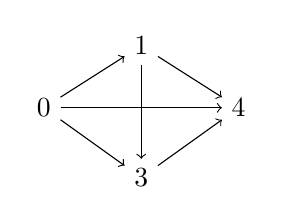
\begin{tikzpicture}[x=1.6em,y=1.4em]
  \node (v1) at (2.2,2.8) {$1$};
  \node (v0) at (0,1.2) {$0$};
  \node (v4) at (4.4,1.2) {$4$};
  \node (v3) at (2.2,-0.6) {$3$};
  \draw[->] (v0) -- (v1);
  \draw[->] (v0) -- (v4);
  \draw[->] (v0) -- (v3);
  \draw[->] (v1) -- (v4);
  \draw[->] (v1) -- (v3);
  \draw[->] (v3) -- (v4);
\end{tikzpicture}
\end{center}
把右手边的\trSimplex{}——即 2-容许 4-\trSimplex{}的第 2 面——诠释为第 3 面与第 1 面的
一个复合是有意义的，因为下列诸\trSimplex{}是薄的：
\begin{center}
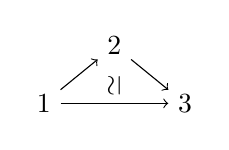
\begin{tikzpicture}[x=1.5em,y=1.3em]
  \node (a) at (0,0) {$1$};
  \node (c) at (3.4,0) {$3$};
  \node (b) at (1.7,1.6) {$2$};
  \draw[->] (a) -- (b);
  \draw[->] (b) -- (c);
  \draw[->] (a) -- (c);
  \node[rotate=90] at (1.7,0.5) {$\simeq$};
\end{tikzpicture}
\qquad
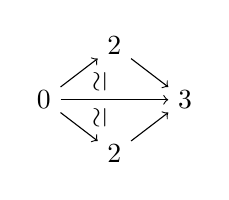
\begin{tikzpicture}[x=1.5em,y=1.3em]
  \node (l) at (0,0) {$0$};
  \node (r) at (3.4,0) {$3$};
  \node (t) at (1.7,1.5) {$2$};
  \node (b) at (1.7,-1.5) {$2$};
  \draw[->] (l) -- (t);
  \draw[->] (t) -- (r);
  \draw[->] (l) -- (r);
  \draw[->] (l) -- (b);
  \draw[->] (b) -- (r);
  \node[rotate=90] at (1.35,0.5) {$\simeq$};
  \node[rotate=90] at (1.35,-0.5) {$\simeq$};
\end{tikzpicture}
\qquad
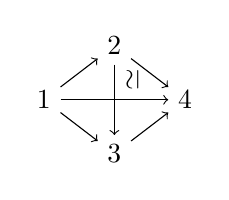
\begin{tikzpicture}[x=1.5em,y=1.3em]
  \node (l) at (0,0) {$1$};
  \node (r) at (3.4,0) {$4$};
  \node (t) at (1.7,1.5) {$2$};
  \node (b) at (1.7,-1.5) {$3$};
  \draw[->] (l) -- (t);
  \draw[->] (t) -- (r);
  \draw[->] (l) -- (b);
  \draw[->] (b) -- (r);
  \draw[->] (l) -- (r);
  \draw[->] (t) -- (b);
  \node[rotate=90] at (2.15,0.55) {$\simeq$};
\end{tikzpicture}
\end{center}
\end{example}

我们把由诸初等带标记\trAnodyneExtension\trCell{}式生成的那些映射称作\textbf{带标记%
\trAnodyneExtension}（marked anodyne extensions）。例如，把求解第 1 章中的%
\cref{ex:free-living-isomorphism} 的论证稍加推广：

\begin{lemma}\label{lem:marked-anodyne-free-isomorphism}
把带标记 1-\trSimplex{}映入极大标记同构的包含
$\qcTwo^{\sharp}\hookrightarrow\qcInt^{\sharp}$ 是一支带标记\trAnodyneExtension，单射
$\qcOne\hookrightarrow\qcInt^{\sharp}$ 亦然。
\end{lemma}

\begin{proof}
见\cref{ex:prove-lem-anodyne}。
\end{proof}

\begin{definition}\label{def:complicial-isofibration}
\trMarkedSimplicialSet{}之间的一个映射是一个\textbf{复状等价纤维化}（complicial
isofibration），若它对诸初等带标记\trAnodyneExtension{}具有右\trLifting{}性质，且其
定义域与余定义域都是复状单纯集。
\end{definition}

由\cref{ex:thinness-for-free}，复状单纯集之间的一个带标记映射是一个复状
等价纤维化，当且仅当它对诸复状号角扩张有\trLifting——诸复状薄性扩张则
自动白得。由附录 C 中的\cref{lem:right-lifting-closure}，复状等价纤维化
随之对一切带标记\trAnodyneExtension{}都具有右\trLifting{}性质。诸\textbf{%
\trTrivialFibration}——被定义为对诸\trMonomorphism{}有\trLifting{}的那些%
\trMarkedSimplicialSet{}之间的映射——也在复状等价纤维化之列，一如%
\cref{lem:mono-marked-cellularly-generated} 所刻画的那样。

「复状单纯集」一词的原初含义指的只是我们如今称作\emph{严格}的那一特定
品种。

\begin{definition}\label{def:strict-complicial-set}
一个\textbf{严格复状单纯集}（strict complicial set）是一个沿诸初等带标记%
\trAnodyneExtension \eqref{eq:complicial-horn-extension} 与
\eqref{eq:complicial-thinness-extension} 容有唯一\trExtension{}的带标记%
\trSimplicialSet{}。
\end{definition}

在手稿 \cite{bib128} 中，\trVerity{}证明了：严格复状单纯集恰是那些作为
严格 $\omega$-范畴的 Street 神经的\trMarkedSimplicialSet{}，从而解决了 Roberts 与
Street 的一个猜想。在本手稿中，我们主要利用\trMarkedSimplicialSet{}来简化关于
拟范畴中\trIsomorphism{}与拟范畴之间的\trEquivalence{}的诸结果的证明。在发展出期间所需的若干组合构造之后，
我们将在 D.4 节与 D.5 节中更明确地讨论这一话题。

\begin{definition}\label{def:n-trivial}
一个\trMarkedSimplicialSet{} $X$ 是 \textbf{$n$-平凡}（$n$-trivial）的，若所有 $r>n$
的 $r$-\trSimplex{}都被标记。
\end{definition}

$n$-平凡\trMarkedSimplicialSet{}的全子范畴在\trMarkedSimplicialSet{}的\trCategory{}中既是反射的
（reflective）又是余反射的（coreflective）：
\begin{center}
\begin{tikzpicture}[x=1.5em,y=1.1em]
  \node (L) at (0,0) {$n\text{-}\sSet^{+}$};
  \node (R) at (4.8,0) {$\sSet^{+}$};
  \draw[->] (3.9,0.32) to[bend right=20] node[pos=0.5,above=10pt]{$\scriptstyle\mathrm{trv}_{n}$} node[pos=0.5,above=1pt]{$\scriptstyle\dashv$} (0.9,0.32);
  \draw[right hook->] (0.7,0) -- (4.1,0);
  \draw[->] (3.9,-0.32) to[bend left=20] node[pos=0.5,below=1pt]{$\scriptstyle\dashv$} node[pos=0.5,below=10pt]{$\scriptstyle\mathrm{core}_{n}$} (0.9,-0.32);
\end{tikzpicture}
\end{center}
也就是说，\textbf{$n$-平凡化}（$n$-trivialization）在 $\sSet^{+}$ 上定义
了一个\trIdempotent{}\trMonad，其单位是\trMarkedSimplicialSet{} $X$ 进入\trMarkedSimplicialSet{}
$\mathrm{trv}_{n}X$ 的\trEntireInclusion{} $X\hookrightarrow_{e}\mathrm{trv}_{n}X$——
后者在维数 $1,\dots,n$ 中与 $X$ 带有相同的带标记\trSimplex{}，而所有更高维的%
\trSimplex{}都「被弄薄」。一个复状单纯集是 $n$-平凡的，若此映射是一个%
\trIsomorphism。

$n$-\textbf{核}（$n$-core）$\mathrm{core}_{n}X$——由限制在那些于 $X$ 中
维数高于 $n$ 的诸面皆为薄的\trSimplex{}上而定义——定义了一个\trIdempotent{}余
单子（comonad），其余单位是正则包含 $\mathrm{core}_{n}X\hookrightarrow_{r}X$。
同样地，一个复状单纯集是 $n$-平凡的，恰好当此映射是一个\trEquivalence。对如
此产生的单子–余单子对而言，这些函子是一对\trAdjunction：
$\mathrm{trv}_{n}\dashv\mathrm{core}_{n}$。

诸 $n$-平凡\trMarkedSimplicialSet{}之子范畴的包含拥有\trAdjunction
\begin{center}
\begin{tikzpicture}[x=1.5em,y=1.1em]
  \node (S) at (0,0) {$\sSet$};
  \node (A) at (2.8,0) {$0\text{-}\sSet^{+}$};
  \node (D1) at (5.2,0) {$\subset\cdots\subset$};
  \node (B) at (7.8,0) {$(n{-}1)\text{-}\sSet^{+}$};
  \node (C) at (11.0,0) {$n\text{-}\sSet^{+}$};
  \node (D2) at (13.4,0) {$\subset\cdots\subset$};
  \node (T) at (15.8,0) {$\sSet^{+}$};
  \draw[->] (S) -- node[pos=0.5,above]{$\scriptstyle(\text{--})^{\sharp}$} node[pos=0.5,below]{$\scriptstyle\simeq$} (A);
  \draw[->] (C) to[bend right=22] node[pos=0.5,above=10pt]{$\scriptstyle\mathrm{trv}_{n-1}$} node[pos=0.5,above=1pt]{$\scriptstyle\dashv$} (B);
  \draw[right hook->] (8.5,0) -- (10.3,0);
  \draw[->] (C) to[bend left=22] node[pos=0.5,below=1pt]{$\scriptstyle\dashv$} node[pos=0.5,below=10pt]{$\scriptstyle\mathrm{core}_{n-1}$} (B);
\end{tikzpicture}
\end{center}
复状单纯集的 $n$-核仍是一个复状单纯集，但 $n$-平凡化函子——它只是在相应的
维数标记\trSimplex{}而不改动底\trSimplicialSet——却不必然保持复状单纯集（见
\cref{ex:n-core-complicial}）。

\begin{remark}[奇对偶]\label{rem:odd-dual}
回顾：一个\trSimplicialSet{} $X$ 的\textbf{\trOppositeSimplicialSet}，是把
$X$ 沿对合 $(-)^{\mathrm{op}}\colon\Delta\to\Delta$——它反转每个序数中的
排序——重新标号而得的\trSimplicialSet{}。这一运算可以自然的方式扩张到\trMarkedSimplicialSet{}上：
在 $X^{\mathrm{op}}$ 中标记一个 $n$-\trSimplex{}，恰好当 $X$ 中相应的 $n$-\trSimplex{}被
标记。然而请注意，按 Street 对 $n$-\trSimplex{}的诠释——它编码一个 $n$ 维态射，
从其诸奇数 $(n-1)$ 维面的复合指向其诸偶数 $(n-1)$ 维面的复合——这一运算
并非简单地反转\trMarkedSimplicialSet{}中「所有胞腔的方向」。毋宁说，它只反转\emph{奇数}
维胞腔中所有\trSimplex{}的方向，而在所有偶数维胞腔中保持方向不变。因此，我们把
这一顶点重排构造称作\trMarkedSimplicialSet{}的\textbf{奇对偶}（odd dual）。
\end{remark}

我们以一段关于复状单纯集之间\trEquivalence{}的讨论作结。

\begin{definition}[复状单纯集的等价]\label{def:complicial-equivalences}
复状单纯集之间的一个映射 $f\colon A\to B$ 是一个\textbf{\trEquivalence}，
若它扩张成一份以带标记 1-\trSimplex{} $\Delta[1]^{\sharp}$ 为\trInterval{}的%
\trHomotopyEquivalence{}数据：\footnote{大体上由
\cref{lem:marked-anodyne-free-isomorphism}，复状单纯集间的\trEquivalence{}%
本可改用带标记\trHomotopyCoherentIsomorphism{} $\qcInt^{\sharp}$ 来定义
（见\cref{cor:complicial-equivalences-hoc}）。但复状单纯集这一高阶范畴模型的优势之一在于：正确的%
\trEquivalence{}概念可以用带标记 1-\trSimplex{}这份更简单的数据来定义。}也就是说，
若存在映射
$g\colon B\to A$，连同
\begin{center}
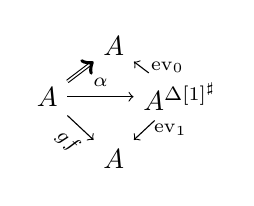
\begin{tikzpicture}[x=1.6em,y=1.4em]
  \node (At) at (1.5,2.4) {$A$};
  \node (Al) at (0,1.1) {$A$};
  \node (M) at (3.0,1.1) {$A^{\Delta[1]^{\sharp}}$};
  \node (Ab) at (1.5,-0.5) {$A$};
  \draw[double,->] (Al) -- (At);
  \draw[->] (Al) -- node[above]{$\scriptstyle\alpha$} (M);
  \draw[->] (M) -- node[right]{$\scriptstyle\mathrm{ev}_{0}$} (At);
  \draw[->] (M) -- node[right]{$\scriptstyle\mathrm{ev}_{1}$} (Ab);
  \draw[->] (Al) -- node[below,sloped]{$\scriptstyle gf$} (Ab);
\end{tikzpicture}
\qquad 与 \qquad
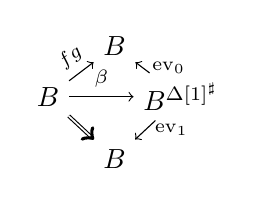
\begin{tikzpicture}[x=1.6em,y=1.4em]
  \node (Bt) at (1.5,2.4) {$B$};
  \node (Bl) at (0,1.1) {$B$};
  \node (M) at (3.0,1.1) {$B^{\Delta[1]^{\sharp}}$};
  \node (Bb) at (1.5,-0.5) {$B$};
  \draw[->] (Bl) -- node[above,sloped]{$\scriptstyle fg$} (Bt);
  \draw[->] (Bl) -- node[above]{$\scriptstyle\beta$} (M);
  \draw[->] (M) -- node[right]{$\scriptstyle\mathrm{ev}_{0}$} (Bt);
  \draw[->] (M) -- node[right]{$\scriptstyle\mathrm{ev}_{1}$} (Bb);
  \draw[double,->] (Bl) -- (Bb);
\end{tikzpicture}
\end{center}
\end{definition}

复状单纯集间等价的数据经转置便给出「带标记\trHomotopyEquivalence」这一更
一般概念的一个实例——对于后者，我们去掉\trMarkedSimplicialSet{}须为复状单纯集的要求。

\begin{definition}\label{def:marked-homotopy}
映射对 $f,g\colon X\to Y$ 之间的一个\textbf{带标记\trHomotopy}（marked
homotopy），由一个映射 $\alpha\colon X\times\Delta[1]^{\sharp}\to Y$ 给出，
它沿端点包含 $X+X\hookrightarrow_{r}X\times\Delta[1]^{\sharp}$ 的限制分别
为映射 $f$ 与 $g$。当 $X$ 与 $Y$ 是极小标记\trSimplicialSet{}时，一个映射
$X\times\Delta[1]\to Y$ 可\trExtension{}为映射
$X\times\Delta[1]^{\sharp}\to Y$，恰好当对每个 0-\trSimplex{} $x\in X$，1-\trSimplex{}
$(x\sigma^{0},\mathrm{id}_{[1]})\in X\times\Delta[1]^{\sharp}$ 被送到 $Y$
的一个退化、从而被标记的 1-\trSimplex{}。\footnote{\trMarkedSimplicialSet{}的\trCartesianProduct{}将在%
\cref{prop:marked-cartesian-closed}中更详细地描述。}
\end{definition}

\textbf{带标记\trHomotopyEquivalence}（marked homotopy equivalence）由
如下数据构成：
\begin{itemize}
\item 一对带标记映射 $f\colon X\to Y$ 与 $g\colon Y\to X$；以及
\item 一对带标记\trHomotopy{} $\alpha\colon X\times\Delta[1]^{\sharp}\to X$
  与 $\beta\colon Y\times\Delta[1]^{\sharp}\to Y$，分别是 $\mathrm{id}_{X}$
  与 $gf$ 之间、以及 $fg$ 与 $\mathrm{id}_{Y}$ 之间的\trHomotopy。
\end{itemize}

当 $X$ 与 $Y$ 是复状单纯集时，带标记\trHomotopy{}可以反转与复合。即便情形
并非如此，我们也容许自己不经说明地反转构成一个带标记\trHomotopyEquivalence{}%
的那些带标记\trHomotopy{}的方向。

\begin{digression}[复状单纯集的 \trVerity{}模型结构]\label{dig:verity-model-structure}
\trMarkedSimplicialSet{}的\trCategory{}带有一个\trCartesianClosed、余纤维性生成的%
\trModelStructure，其\trFibrant{}对象恰是诸复状单纯集，而其诸余纤维化恰为诸%
\trMonomorphism{} \cite[\S6.2-4]{bib129}。在纤维性对象之间，诸\trFibration{}%
与诸\trWeakEquivalence{}恰是上文定义的复状等价纤维化类与\trEquivalence{}类。
在以下各节中，我们直接对纤维性对象范畴验证其中的许多性质，只把%
\trModelStructure{}本身的验证留给文献——它由 Jeff Smith 定理得出。
\end{digression}

\subsection*{练习}

\begin{exercise}\label{ex:prove-lem-mono-generated}
证明\cref{lem:mono-marked-cellularly-generated}。
\end{exercise}

\begin{exercise}\label{ex:maximally-marked-kan}
证明：一个极大标记\trSimplicialSet{}定义一个复状单纯集，当且仅当其底\trSimplicialSet{}%
是一个\trKanComplex。
\end{exercise}

\begin{exercise}\label{ex:prove-lem-anodyne}
证明\cref{lem:marked-anodyne-free-isomorphism}。
\end{exercise}

\begin{exercise}\label{ex:thinness-for-free}
设 $f\colon A\to B$ 是\trMarkedSimplicialSet{}之间的任一映射，其定义域 $A$ 是一个
复状单纯集。证明：$f$ 对诸复状薄性扩张具有（唯一的）右\trLifting{}性质。
\end{exercise}

\begin{exercise}\label{ex:n-core-complicial}
\begin{enumerate}[label=(\roman*)]
\item 证明：一个复状单纯集的 $n$-核是一个复状单纯集。
\item 找出一个复状单纯集的例子，使其对某个 $n$ 的 $n$-平凡化不再是复状%
  \trSimplicialSet{}。
\end{enumerate}
\end{exercise}

   %

\providecommand{\sSet}{s\mathcal{S}et}%
\providecommand{\qcTwo}{\mathbf{2}}%


\section{联接与切片构造}\label{sec:the-join-and-slice-constructions}

在本节中，我们远比第 4 章中的\cref{def:join}所给出的更为详细地重访 Joyal 的%
\textbf{\trJoin}（join）与\textbf{切片}构造，并讨论它们向\trMarkedSimplicialSet{}的%
扩张。我们证明：\trMonomorphism{}以及几类\trAnodyne（anodyne）映射的 Leibniz \trJoin{}仍%
定义同种类型的\trMonomorphism。
如果我们以\emph{增广}单纯集代替通常的单纯集来工作，组合上的处理会稍微%
容易一些——这一进路沿循 Ehlers 与 Porter \cite{bib40} 对\trSimplicial\trJoin{}的原始定义。

\begin{definition}[序数和]\label{def:ordinal-sum}
代数学家的、由有限序数与保序映射构成的骨架范畴 $\Delta_{+}$——其对象为%
$[n]=\{0\le 1\le\cdots\le n\}$ 与 $[-1]=\varnothing$——承载一个严格（非对称）%
幺半结构 $(\Delta_{+},\oplus,[-1])$，其中 $\oplus$ 表示如下定义的%
\textbf{序数和}（ordinal sum）：
\begin{itemize}
\item 对对象 $[n],[m]\in\Delta_{+}$，令 $[n]\oplus[m]:=[n+1+m]$；
\item 对箭头 $\alpha\colon[n]\to[n']$、$\beta\colon[m]\to[m']$，令
$\alpha\oplus\beta\colon[n+1+m]\to[n'+1+m']$ 由
\begin{equation*}
\alpha\oplus\beta(i)=
\begin{cases}
\alpha(i) & \text{若 } i\le n,\\
\beta(i-n-1)+n'+1 & \text{否则}
\end{cases}
\end{equation*}
给出。
\end{itemize}
\end{definition}

经 Day 卷积\cite{bib33}，\trJoin\trBifunctor
$\oplus\colon\Delta_{+}\times\Delta_{+}\to\Delta_{+}$ 扩张成增广单纯集的%
\trCategory{} $\sSet_{+}:=\mathcal{S}et^{\Delta_{+}^{\mathrm{op}}}$ 上的一个%
（非对称）幺半封闭结构
\begin{equation*}
(\sSet_{+},\star,\Delta[-1],\mathrm{dec}_{l},\mathrm{dec}_{r})\mbox{.}
\end{equation*}

\begin{definition}[增广单纯集的\trJoin]\label{def:join-augmented-simplicial-sets}
增广单纯集 $X$ 与 $Y$ 的\textbf{\trJoin} $X\star Y$ 可显式描述如下：
\begin{itemize}
\item 它的诸单纯形是二元组 $(x,y)\in(X\star Y)_{r+1+s}$，其中 $x\in X_{r}$、%
$y\in Y_{s}$。
\item 设 $(x,y)$ 是 $X\star Y$ 的一个单纯形，其中 $x\in X_{r}$、$y\in Y_{s}$，%
又设 $\alpha\colon[n]\to[r+1+s]$ 是 $\Delta_{+}$ 中的一个单纯算子，则 $\alpha$%
可唯一地分解为 $\alpha=\alpha_{1}\oplus\alpha_{2}$，其中%
$\alpha_{1}\colon[n_{1}]\to[r]$、$\alpha_{2}\colon[n_{2}]\to[s]$，并且%
$(x,y)\cdot\alpha:=(x\cdot\alpha_{1},\,y\cdot\alpha_{2})$。
\end{itemize}
\end{definition}

由构造即见 $\Delta[n]\star\Delta[m]\cong\Delta[n+1+m]$，因为%
$[n]\oplus[m]=[n+1+m]$。%
\footnote{Day 卷积积的一个一般性特征是：Yoneda 嵌入%
$\mathcal{Y}\colon\Delta_{+}\hookrightarrow\mathcal{S}et^{\Delta_{+}^{\mathrm{op}}}$%
定义一个强幺半函子。}

注意 $\Delta[-1]$——即那个仅有单个 $-1$-单纯形而无其他单纯形的带标记%
\trSimplicialSet——是\trJoin\trBifunctor{}的一个双侧单位。
\footnote{译注：此处照录原书面貌。就上下文而言，$\Delta[-1]$ 作为%
$(\sSet_{+},\star)$ 的单位乃是\emph{增广}单纯集，原文作「marked simplicial
set」，疑为「augmented simplicial set」之误。}

\begin{definition}[增广单纯集的错位]\label{def:decalage}
两个闭构造 $\mathrm{dec}_{l}$ 与 $\mathrm{dec}_{r}$——分别称作\textbf{左错位%
构造}与\textbf{右错位构造}（left and right décalage constructions）——定义为%
\trJoin{}的参数化\trRightAdjoint：
\begin{center}
\begin{tikzpicture}[x=1.4em,y=1.3em]
  \node (l1) at (0,0) {$\sSet_{+}$};
  \node (r1) at (7.2,0) {$\sSet_{+}$};
  \draw[->] (1.2,0.45) to[bend left=20] node[above]{$\scriptstyle X\star-$} (6.0,0.45);
  \node at (3.6,0) {$\dashv$};
  \draw[->] (6.0,-0.45) to[bend left=20] node[below]{$\scriptstyle\mathrm{dec}_{l}(X,-)$} (1.2,-0.45);
  \node at (10.2,0) {与};
  \begin{scope}[shift={(13.2,0)}]
  \node (l2) at (0,0) {$\sSet_{+}$};
  \node (r2) at (7.2,0) {$\sSet_{+}$};
  \draw[->] (1.2,0.45) to[bend left=20] node[above]{$\scriptstyle-\star X$} (6.0,0.45);
  \node at (3.6,0) {$\dashv$};
  \draw[->] (6.0,-0.45) to[bend left=20] node[below]{$\scriptstyle\mathrm{dec}_{r}(X,-)$} (1.2,-0.45);
  \end{scope}
\end{tikzpicture}
\end{center}
从而存在由诸\trBifunctor{}构成的一个双变量伴随：
\begin{gather*}
\sSet_{+}\times\sSet_{+}
  \xrightarrow{\ -\star-\ }
\sSet_{+},\\
\sSet_{+}^{\mathrm{op}}\times\sSet_{+}
  \xrightarrow{\ \mathrm{dec}_{l}(-,-)\ }
\sSet_{+},
\qquad
\sSet_{+}^{\mathrm{op}}\times\sSet_{+}
  \xrightarrow{\ \mathrm{dec}_{r}(-,-)\ }
\sSet_{+}\mbox{.}
\end{gather*}
\end{definition}

\begin{observation}[单纯集与增广单纯集]\label{obs:ssets-vs-augmented-ssets}
遗忘增广的显然函子 $U\colon\sSet_{+}\to\sSet$ 同时容许\trLeftAdjoint{}与%
\trRightAdjoint
\begin{center}
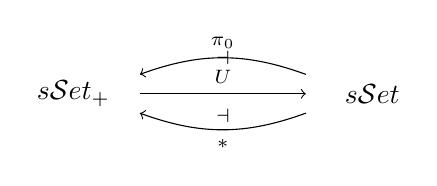
\begin{tikzpicture}[x=1.5em,y=1.4em]
  \node (l) at (0,0) {$\sSet_{+}$};
  \node (r) at (7.2,0) {$\sSet$};
  \draw[->] (5.6,0.5) to[bend right=20] node[above]{$\scriptstyle\pi_{0}$} (1.6,0.5);
  \draw[->] (1.6,0) -- node[pos=0.5,above=7pt]{$\scriptstyle\dashv$} node[above]{$\scriptstyle U$} node[pos=0.5,below=2pt]{$\scriptstyle\dashv$} (5.6,0);
  \draw[->] (5.6,-0.5) to[bend left=20] node[below]{$\scriptstyle\ast$} (1.6,-0.5);
\end{tikzpicture}
\end{center}
其中\trLeftAdjoint{}以 $\pi_{0}X$ 增广一个单纯集 $X$，这里 $\pi_{0}X$ 是由%
余等化子
\begin{equation*}
X_{1}
\;\;\mathop{\mathclap{\substack{\textstyle\delta^{1}\\\longrightarrow\\[-0.6ex]\textstyle\delta^{0}\\[-0.6ex]\longrightarrow}}}\;\;
X_{0}
\;\longrightarrow\;
\pi_{0}X
\end{equation*}
定义的路径分量集，而右伴随则通过添加单个 $-1$-单纯形来以「终」方式增广%
一个单纯集。$\pi_{0}\dashv U$ 的\trUnit{}与 $U\dashv\ast$ 的\trCounit{}都是%
\trIsomorphism；因此任一\trAdjunction{}都定义一个\trFullyFaithful{}嵌入%
$\sSet\hookrightarrow\sSet_{+}$。
\end{observation}

任何增广单纯集都典范地是其「终增广」的诸\textbf{分支}的一个\trCoproduct：
\begin{lemma}\label{lem:components-decomposition}
设 $X$ 是一个增广单纯集。
\begin{enumerate}[label=(\roman*)]
\item 对每个 $i\in X_{-1}$，由任意维数中其 $-1$-单纯形面为 $i$ 的那些单纯形%
所组成的子集 $X_{\langle i\rangle}$ 构成 $X$ 的一个终增广单纯子集。
\item 这些分支的无交并
$\coprod_{i\in X_{-1}}X_{\langle i\rangle}$ \trIsomorphism{}于 $X$。
\end{enumerate}
\end{lemma}

\begin{proof}
\cref{ex:components-decomposition-exercise}。
\end{proof}

\begin{definition}[单纯集的\trJoin]\label{def:join-simplicial-sets}
依约定，一对单纯集的\textbf{\trJoin}定义为诸平凡增广单纯集之\trJoin{}的底单纯集。
于是，\trJoin\trBifunctor{}是复合
\begin{center}
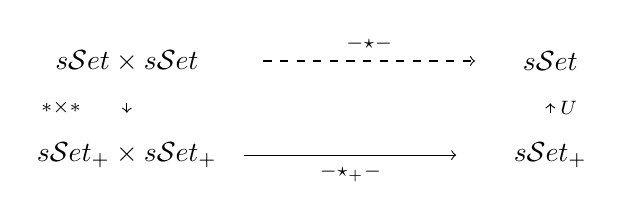
\begin{tikzpicture}[x=1.7em,y=1.7em]
  \node (tl) at (0,2) {$\sSet\times\sSet$};
  \node (tr) at (9,2) {$\sSet$};
  \node (bl) at (0,0) {$\sSet_{+}\times\sSet_{+}$};
  \node (br) at (9,0) {$\sSet_{+}$};
  \draw[->,dashed] (2.9,2) -- node[above]{$\scriptstyle-\star-$} (7.4,2);
  \draw[->] (0,1.1) -- (0,0.9);
  \node at (-1.4,1.0) {$\scriptstyle\ast\times\ast$};
  \draw[->] (9,0.9) -- node[right]{$\scriptstyle U$} (9,1.1);
  \draw[->] (2.5,0) -- node[below]{$\scriptstyle-\star_{+}-$} (7.0,0);
\end{tikzpicture}
\end{center}
显式地，$X\star Y$ 的 $n$-单纯形是由 $X$ 的一个 $j$-单纯形与 $Y$ 的一个%
$k$-单纯形组成的二元组，其中 $j+k=n-1$；当 $j=-1$ 时，这样的「二元组」
恰由 $Y$ 的单个 $n$-单纯形构成，而当 $k=-1$ 时，则恰由 $X$ 的单个%
$n$-单纯形构成。这便恢复了第 4 章中的\cref{def:join}。
\end{definition}

正如第 4 章中的\cref{def:join}所观察到的，单纯集 $X$ 与 $Y$ 的\trJoin{}容许%
典范嵌入
\begin{equation*}
X\hookrightarrow X\star Y\hookleftarrow Y
\end{equation*}
这些嵌入可理解为：把 $X\star-$ 与 $-\star Y$ 分别作用于 $\sSet_{+}$ 中在诸%
平凡增广里挑出唯一 $-1$-单纯形的那些映射 $\Delta[-1]\to Y$ 与%
$\Delta[-1]\to X$ 所得的映射。

\begin{lemma}\label{lem:join-colimits}
\begin{enumerate}[label=(\roman*)]
\item \trJoin\trBifunctor{} $-\star-\colon\sSet\times\sSet\to\sSet$ 在每个变量%
中都保持连通余极限。
\item 对任何单纯集 $X$，诸\trJoin\trFunctor
\begin{equation*}
\sSet\xrightarrow{\ X\star-\ }X/\sSet
\qquad\text{与}\qquad
\sSet\xrightarrow{\ -\star X\ }X/\sSet
\end{equation*}
保持一切\trColimit。
\end{enumerate}
\end{lemma}

\begin{proof}
在\cref{def:join-simplicial-sets}中，单纯集的\trJoin{}被定义为三个\trFunctor{}的%
复合，其中有两个\trFunctor{}拥有\trRightAdjoint，从而保持一切\trColimit。%
第三个\trFunctor{} $\ast\colon\sSet\to\sSet_{+}$ 不拥有\trRightAdjoint，但%
从下述定义看得出它仍保持\emph{连通}余极限：一个标号 $1$-\trCategory{} $J$
是连通的，当且仅当取值于单点集的常值 $J$-标号图表的余极限是单点集。这就%
证明了 (i)。

现在，\trForgetfulFunctor{} $X/\sSet\to\sSet$ 严格地创造连通余极限%
\cite[3.3.8]{bib104}，故 (ii) 中的诸\trJoin\trFunctor{}保持连通余极限。任意%
\trColimit{}都可由连通余极限与\trCoproduct{}构造出来，因此为证 (ii)，只剩%
下论证这些\trFunctor{}保持\trCoproduct。虽然若把%
$\coprod_{i}(X\star Y_{i})$ 解释为 $\sSet$ 中的余积，则%
$X\star(\coprod_{i}Y_{i})\ncong\coprod_{i}(X\star Y_{i})$，但可以直接验证：%
$X\star(\coprod_{i}Y_{i})$ 是 $\coprod_{i}(X\star Y_{i})$ 模去把每一个包含%
$X\hookrightarrow X\star Y_{i}$ 的像等同于 $X$ 的单个副本所得的商，而这恰是%
$X/\sSet$ 中余积的构造。
\end{proof}

\begin{definition}[单纯集的切片]\label{def:slices-of-simplicial-sets}
范畴 $\sSet$ 与 $X/\sSet$ 都是局部可表现的，故\cref{lem:join-colimits}(ii)%
的诸\trCocomplete{}函子都拥有\trRightAdjoint（见\cite[1.57]{bib1}），这些右%
伴随在 $f\colon X\to A$ 处的值定义了 Joyal 的\textbf{切片单纯集}（sliced simplicial
sets）${}^{f/}\!A$ 与 $A_{/f}$，它们由第 4 章中的%
\cref{prop:join-slice-adjunction}所描述的诸\trUniversalProperty{}刻画：
\begin{gather*}
\mbox{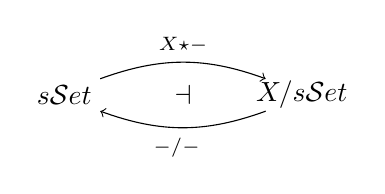
\begin{tikzpicture}[x=1.3em,y=1.3em]
  \node (l) at (0,0) {$\sSet$};
  \node (r) at (6.6,0) {$X/\sSet$};
  \draw[->] (1.0,0.45) to[bend left=20] node[above]{$\scriptstyle X\star-$} (5.6,0.45);
  \node at (3.3,0) {$\dashv$};
  \draw[->] (5.6,-0.45) to[bend left=20] node[below]{$\scriptstyle-/-\;\;{}$} (1.0,-0.45);
\end{tikzpicture}}
\qquad
\left\{\,Y\to{}^{f/}\!A\,\right\}:=
\left\{\vcenter{\hbox{\begin{tikzpicture}[x=1.2em,y=1.2em]
  \node (x) at (1.4,0.9) {$X$};
  \node (a) at (4.2,0) {$A$};
  \node (xy) at (0,-0.9) {$X\star Y$};
  \draw[->] (2.2,0.78) -- (3.8,0.25);
  \node at (3.3,0.75) {$\scriptstyle f$};
  \draw[right hook->] (1.0,0.4) -- (0.4,-0.5);
  \draw[->] (1.2,-0.9) -- (3.2,-0.35);
\end{tikzpicture}}}\right\} \\[0.8em]
\mbox{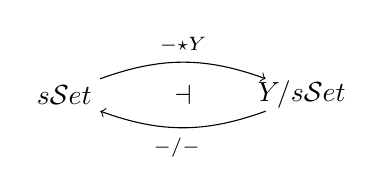
\begin{tikzpicture}[x=1.3em,y=1.3em]
  \node (l) at (0,0) {$\sSet$};
  \node (r) at (6.6,0) {$Y/\sSet$};
  \draw[->] (1.0,0.45) to[bend left=20] node[above]{$\scriptstyle-\star Y$} (5.6,0.45);
  \node at (3.3,0) {$\dashv$};
  \draw[->] (5.6,-0.45) to[bend left=20] node[below]{$\scriptstyle-/-\;\;{}$} (1.0,-0.45);
\end{tikzpicture}}
\qquad
\left\{\,X\to A_{/g}\,\right\}:=
\left\{\vcenter{\hbox{\begin{tikzpicture}[x=1.2em,y=1.2em]
  \node (y) at (1.4,0.9) {$Y$};
  \node (a) at (4.2,0) {$A$};
  \node (xy) at (0,-0.9) {$X\star Y$};
  \draw[->] (2.2,0.78) -- (3.8,0.25);
  \node at (3.3,0.75) {$\scriptstyle g$};
  \draw[right hook->] (1.0,0.4) -- (0.4,-0.5);
  \draw[->] (1.2,-0.9) -- (3.2,-0.35);
\end{tikzpicture}}}\right\}\mbox{.}
\end{gather*}
\end{definition}

我们把切片 ${}^{f/}\!A$ 想成\textbf{\trDiagram{} $f$ 之下的诸\trCone}的单纯集，
而把对偶切片 $A_{/f}$ 想成\textbf{\trDiagram{} $f$ 之上的诸\trCone}的单纯集。
这一术语与第 4 章中的\cref{def:infinity-category-of-cones}的术语之间的调和
将在\cref{prop:slices-cones-equivalence}中给出。
我们还能经由\cref{lem:components-decomposition}从\cref{def:decalage}的%
错位构造中恢复这些切片单纯集：

\begin{lemma}\label{lem:slices-as-components}
对任何单纯映射 $f\colon X\to A$，单纯集 ${}^{f/}\!A$ 与 $A_{/f}$ 分别是%
$\mathrm{dec}_{l}(X,A)$ 与 $\mathrm{dec}_{r}(X,A)$ 的、由 $-1$-单纯形%
$f\colon X\to A$ 所标引的终增广分支。
\end{lemma}

\begin{proof}
我们把单纯集 $X$ 与 $A$ 等同于它们的终增广单纯集。回顾%
$\Delta[-1]$ 是 $\sSet_{+}$ 上\trJoin\trBifunctor{}的幺半单位。于是，由%
\trAdjunction{}性，映射%
$\Delta[-1]\to\mathrm{dec}_{l}(X,A)$ 或 $\Delta[-1]\to\mathrm{dec}_{r}(X,A)$%
对应于映射 $X\to A$。对另一个终增广单纯集 $Y$，沿\cref{def:decalage}的%
\trAdjunction{}作转置便给出一个对应：
\begin{equation*}
\left\{\vcenter{\hbox{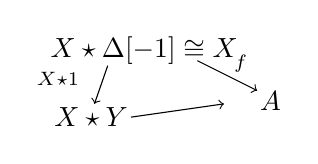
\begin{tikzpicture}[x=1.2em,y=1.2em]
  \node (t) at (1.6,1.0) {$X\star\Delta[-1]\cong X$};
  \node (a) at (5.4,-0.5) {$A$};
  \node (xy) at (0,-1.0) {$X\star Y$};
  \draw[->] (3.2,0.7) -- (5.0,-0.2);
  \node at (4.5,0.6) {$\scriptstyle f$};
  \draw[->] (0.5,0.55) -- (0.1,-0.6);
  \node at (-1.0,0.15) {$\scriptstyle X\star 1$};
  \draw[->] (1.2,-1.0) -- (4.0,-0.6);
\end{tikzpicture}}}\right\}
\cong
\left\{\vcenter{\hbox{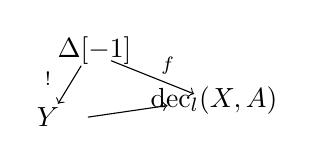
\begin{tikzpicture}[x=1.2em,y=1.2em]
  \node (t) at (1.4,1.0) {$\Delta[-1]$};
  \node (y) at (0,-1.0) {$Y$};
  \node (d) at (5.0,-0.5) {$\mathrm{dec}_{l}(X,A)$};
  \draw[->] (1.0,0.55) -- (0.3,-0.6);
  \node at (0.0,0.15) {$\scriptstyle !$};
  \draw[->] (1.9,0.7) -- (4.4,-0.3);
  \node at (3.6,0.55) {$\scriptstyle f$};
  \draw[->] (1.2,-1.0) -- (3.6,-0.65);
\end{tikzpicture}}}\right\}
\end{equation*}
这便表明 $\mathrm{dec}_{l}(X,A)$ 中由其 $-1$-单纯形面为 $f$ 的那些单纯形%
组成的单纯子集，具有定义 ${}^{f/}\!A$ 的那个\trUniversalProperty。对偶论证%
表明 $\mathrm{dec}_{r}(X,A)$ 中由其 $-1$-单纯形面为 $f$ 的那些单纯形组成的%
单纯子集，具有定义 $A_{/f}$ 的那个\trUniversalProperty。换言之，这些错位%
容许如下的、作为诸切片（终增广的）之无交并的典范分解：
\begin{equation*}
\mathrm{dec}_{r}(X,A)=\coprod_{f\colon X\to A}A_{/f}
\qquad
\mathrm{dec}_{l}(X,A)=\coprod_{f\colon X\to A}{}^{f/}\!A
\end{equation*}
\end{proof}

\begin{definition}[（左／右／内）\trAnodyneExtension]\label{def:anodyne-extensions}
\begin{itemize}
\item 对 $n\ge 1$ 与 $0\le k\le n$ 的诸\textbf{\trHorn{}包含}%
$\Lambda^{k}[n]\hookrightarrow\Delta[n]$ 之集胞腔式地生成\textbf{\trAnodyneExtension}。
\item 对 $n\ge 1$ 与 $0\le k<n$ 的诸\textbf{左\trHorn{}包含}%
$\Lambda^{k}[n]\hookrightarrow\Delta[n]$ 之集胞腔式地生成\textbf{左\trAnodyneExtension}。
\item 对 $n\ge 1$ 与 $0<k\le n$ 的诸\textbf{右\trHorn{}包含}%
$\Lambda^{k}[n]\hookrightarrow\Delta[n]$ 之集胞腔式地生成\textbf{右\trAnodyneExtension}。
\item 对 $n\ge 2$ 与 $0<k<n$ 的诸\textbf{内\trHorn{}包含}%
$\Lambda^{k}[n]\hookrightarrow\Delta[n]$ 之集胞腔式地生成\textbf{内\trAnodyneExtension}。
\end{itemize}
\end{definition}

我们把对这些映射具有右\trLifting{}性质的右类分别称为\textbf{\trKanFibration}、%
\textbf{\trLeftFibration}、\textbf{\trRightFibration}与\textbf{\trInnerFibration}。
由一个容易的直接计算：

\begin{lemma}\label{lem:leibniz-join-horn-boundary}
\emph{一个\trHorn{}包含与一个\trBoundary{}包含的 Leibniz \trJoin\trIsomorphism{}于%
单个\trHorn{}包含}：
\begin{gather*}
(\Lambda^{k}[n]\hookrightarrow\Delta[n])\mathbin{\hat{\star}}
(\partial\Delta[m]\hookrightarrow\Delta[m])
\cong
\Lambda^{k}[n+1+m]\hookrightarrow\Delta[n+1+m]\mbox{,}\\
(\partial\Delta[n]\hookrightarrow\Delta[n])\mathbin{\hat{\star}}
(\Lambda^{k}[m]\hookrightarrow\Delta[m])
\cong
\Lambda^{n+k+1}[n+1+m]\hookrightarrow\Delta[n+1+m]\mbox{.}
\end{gather*}
\end{lemma}

\begin{proof}
由于\trJoin\trBifunctor{}是序数和的 Day 卷积，且 $[n]\oplus[m]=[n+1+m]$，故%
$\Delta[n]\star\Delta[m]\cong\Delta[n+1+m]$。第一个 Leibniz 张量的定义域是%
单纯集
\begin{equation*}
\Lambda^{k}[n]\star\Delta[m]
\;\underset{\Lambda^{k}[n]\star\partial\Delta[m]}{\cup}\;
\Delta[n]\star\partial\Delta[m]\mbox{.}
\end{equation*}
我们用\cref{def:join-augmented-simplicial-sets}把它等同于%
$\Delta[n+1+m]$ 的一个单纯子集。由于 $\partial\Delta[m]$ 包含 $\Delta[m]$%
的全部余维一的面，$\Delta[n]\star\partial\Delta[m]$ 这一分支便包含%
$\Delta[n+1+m]$ 的对每个指标 $j>n$ 的第 $j$ 个面。类似地，由于%
$\Lambda^{k}[n]$ 包含 $\Delta[n]$ 的除一个之外的全部余维一面，%
$\Lambda^{k}[n]\star\Delta[m]$ 这一分支便包含 $\Delta[n+1+m]$ 的对每个指标%
$i\le n$（$i=k$ 除外）的第 $i$ 个面。于是我们看到，只缺第 $k$ 个面与那个%
$n+1+m$-单纯形，这使我们能够把这个 Leibniz \trJoin{}的定义域等同于号角%
$\Lambda^{k}[n+1+m]$。
\end{proof}

从而：

\begin{corollary}\label{cor:slices-are-quasi-categories}
\emph{若 $f\colon X\to A$ 是任一单纯映射且 $A$ 是一个\trQuasiCategory，则%
${}^{f/}\!A$ 与 $A_{/f}$ 都是\trQuasiCategory}。
\end{corollary}

\begin{proof}
由\cref{lem:slices-as-components}，为证 ${}^{f/}\!A$ 是一个%
\trQuasiCategory，只需证明增广单纯集 $\mathrm{dec}_{l}(X,A)$ 对一切内号角%
容许填充体，这里诸内号角被视为平凡增广单纯集。为此，只需解出转置后的%
\trLifting{}问题，并论证 $A$ 沿如下 Leibniz \trJoin（$n\ge 2$、$0<k<n$）%
容许扩张：
\begin{center}
\begin{tikzpicture}[x=1.6em,y=1.6em]
  \node (a) at (0,1.6) {$\Lambda^{k}[n]$};
  \node (b) at (4.8,1.6) {$\mathrm{dec}_{l}(X,A)$};
  \node (c) at (0,-1.6) {$\Delta[n]$};
  \draw[->] (1.4,1.6) -- (3.2,1.6);
  \draw[right hook->] (0,0.9) -- (0,-0.7);
  \draw[->,dashed] (0.5,-1.2) -- (3.9,1.25);
  \node at (7.4,0) {$\leftrightsquigarrow$};
  \begin{scope}[shift={(10.2,0)}]
  \node (a2) at (0,1.6) {$X\star\Lambda^{k}[n]$};
  \node (b2) at (4.8,1.6) {$A$};
  \node (c2) at (0,-1.6) {$X\star\Delta[n]$};
  \draw[->] (2.5,1.6) -- (3.7,1.6);
  \draw[right hook->] (0,0.9) -- (0,-0.7);
  \draw[->,dashed] (0.5,-1.2) -- (4.1,1.3);
  \end{scope}
\end{tikzpicture}
\end{center}
由\cref{lem:mono-epi-reedy-sset}，包含 $\varnothing\hookrightarrow X$ 由诸%
包含 $\partial\Delta[m]\hookrightarrow\Delta[m]$（$m\ge 0$）胞腔式地生成；%
而由\cref{lem:leibniz-join-horn-boundary}，这些映射与内号角包含的 Leibniz
\trJoin{}都是内\trAnodyneExtension。于是，由\cref{prop:leibniz-construction-preserves}(vii)，%
Leibniz \trJoin%
$(\varnothing\hookrightarrow X)\mathbin{\hat{\star}}(\Lambda^{k}[n]\hookrightarrow\Delta[n])$
便是\trInnerAnodyne{}的，故右上方的\trLifting{}问题容许一个解，该解经转置便定义出%
左上方\trLifting{}问题的一个解。
\end{proof}

我们的下一个目标是证明：诸切片\trQuasiCategory{}等价于 4.2 节中引入的%
诸锥\trQuasiCategory。正如该节所概述的，这一结果的关键在于\trJoin{}构造与%
第 4 章中的\cref{def:fat-join}的所谓「\trFatJoin」构造之间的一个合适的%
\trEquivalence，我们现在就把后者扩张到增广单纯集。
由\cref{lem:components-decomposition}回顾：一个增广单纯集 $X$ 典范地分解为%
诸终增广单纯集的一个余积
$X\cong\coprod_{i\in X_{-1}}X_{\langle i\rangle}$，由 $-1$-单纯形之集所标引。

\begin{definition}[增广单纯集的\trFatJoin{}与错位]\label{def:fat-join-augmented}
对增广单纯集 $X\cong\coprod_{i\in X_{-1}}X_{\langle i\rangle}$ 与%
$Y\cong\coprod_{j\in Y_{-1}}Y_{\langle j\rangle}$，它们的\textbf{\trFatJoin}由%
如下\trPushout{}构造：
\begin{center}
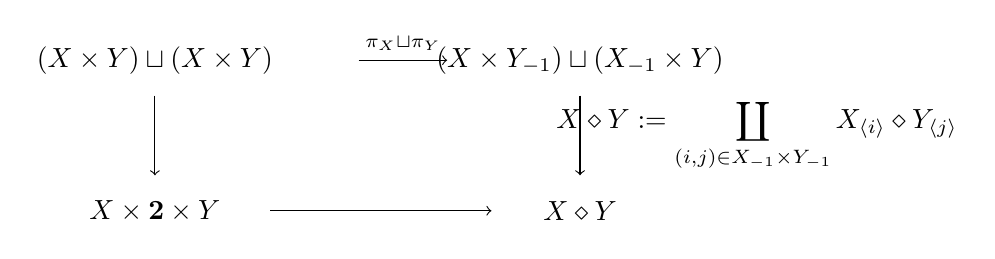
\begin{tikzpicture}[x=1.6em,y=1.6em]
  \node (tl) at (0,1.7) {$(X\times Y)\sqcup(X\times Y)$};
  \node (tr) at (9.6,1.7) {$(X\times Y_{-1})\sqcup(X_{-1}\times Y)$};
  \node (bl) at (0,-1.7) {$X\times\qcTwo\times Y$};
  \node (br) at (9.6,-1.7) {$X\diamond Y$};
  \draw[->] (4.6,1.7) -- node[above]{$\scriptstyle\pi_{X}\sqcup\pi_{Y}$} (6.6,1.7);
  \draw[->] (0,0.9) -- (0,-0.9);
  \draw[->] (9.6,0.9) -- (9.6,-0.9);
  \draw[->] (2.6,-1.7) -- (7.6,-1.7);
  \node at (3.4,0) {$\scriptstyle\ulcorner$};
  \node at (13.6,0)
    {$\displaystyle X\diamond Y:=\coprod_{(i,j)\in X_{-1}\times Y_{-1}}X_{\langle i\rangle}\diamond Y_{\langle j\rangle}$};
\end{tikzpicture}
\end{center}
其中 $X_{\langle i\rangle}\diamond Y_{\langle j\rangle}$ 是由第 4 章中的%
\cref{def:fat-join}的\trFatJoin{}所定义的终增广单纯集。这一构造的安排使得%
\trBifunctor{} $-\diamond-\colon\sSet_{+}\times\sSet_{+}\to\sSet_{+}$ 在每个
变量中都保持一切\trColimit，而不只是\trBifunctor{} $-\diamond-\colon\sSet\times\sSet\to\sSet$
所保持的那些连通余极限。
\end{definition}

显式地，$n$-单纯形之集 $(X\diamond Y)_{n}$ 是 $X\times\qcTwo\times Y$ 的%
$n$-单纯形之集 $X_{n}\times\Delta([n],[1])\times Y_{n}$ 模去如下等同三元组%
的关系所得的商：
\begin{itemize}
\item $(x,0,y)\sim(x,0,y')$，其中 $0\colon[n]\to[1]$ 是常值算子，而 $y$ 与%
$y'$ 位于 $Y\cong\coprod_{j\in Y_{-1}}Y_{\langle j\rangle}$ 的同一分支中；%
并且
\item $(x,1,y)\sim(x',1,y)$，其中 $1\colon[n]\to[1]$ 是常值算子，而 $x$ 与%
$x'$ 位于 $X\cong\coprod_{i\in X_{-1}}X_{\langle i\rangle}$ 的同一分支中。
\end{itemize}

由余连续性与伴随函子定理，$\sSet_{+}$ 上的\trFatJoin\trBifunctor{}同时拥有左闭与%
右闭 $\mathrm{fatdec}_{l}(X,A)$ 与 $\mathrm{fatdec}_{r}(X,A)$，分别称作%
\textbf{左胖错位}与\textbf{右胖错位}（left and right fat décalage）；我们%
以如下约定固定其手性：若 $X$ 是增广单纯集，则
$X\diamond-\dashv\mathrm{fatdec}_{l}(X,-)$ 且
$-\diamond X\dashv\mathrm{fatdec}_{r}(X,-)$。

从\trFatJoin{}到\trJoin{}存在一个典范的比较映射，正如围绕第 4 章中的%
\cref{prop:join-vs-fat-join}的讨论所预告的那样。

\begin{lemma}\label{lem:fat-join-comparison}
\emph{存在增广单纯集的一个典范映射
\begin{equation*}
s^{X,Y}\colon X\diamond Y\to X\star Y
\end{equation*}
它关于 $X$ 与 $Y$ 自然，特别地定义了一个\trNaturalTransformation
\begin{equation*}
s^{n,m}\colon\Delta[n]\diamond\Delta[m]\to\Delta[n]\star\Delta[m]
\qquad\in\sSet_{+}^{\Delta_{+}\times\Delta_{+}}
\end{equation*}
它在 $n$ 或 $m$ 等于 $-1$ 时是\trIsomorphism，%
\footnote{注意
$X\diamond\Delta[-1]\cong X\star\Delta[-1]\cong X\cong\Delta[-1]\diamond X\cong\Delta[-1]\star X$。}
否则则由其在顶点上的保序作用所定义的映射之商而产生：}
\begin{equation*}
\begin{aligned}
\Delta[n]\times\Delta[1]\times\Delta[m]
&\;\xrightarrow{\ \bar{s}^{n,m}\ }\;
\Delta[n+1+m]\\
(i,0,k)&\;\longmapsto\; i\\
(i,1,k)&\;\longmapsto\; k+n+1
\end{aligned}
\end{equation*}
\end{lemma}

注意 $\bar{s}^{n,m}$ 把在\cref{def:fat-join-augmented}中所描述的\trCongruence{}%
之下相关的诸单纯形送到同一个单纯形，从而在商单纯集上诱导出唯一的映射%
$s^{n,m}\colon\Delta[n]\diamond\Delta[m]\to\Delta[n]\star\Delta[m]$。在%
证明中，我们将给出映射 $s^{X,Y}$ 的一个一般构造，它可以被证明在 $X$ 与%
$Y$ 为标准单纯形的情形下与这一描述相合。

\begin{proof}
把集合 $X_{-1}$ 等同于增广单纯集
$\coprod_{X_{-1}}\Delta[-1]$，\trYonedaLemma{}提供了一个增广单纯集的典范%
映射 $X_{-1}\to X$，由此产生一个典范映射
\begin{rveq}\label{eq:fat-join-comparison-map}
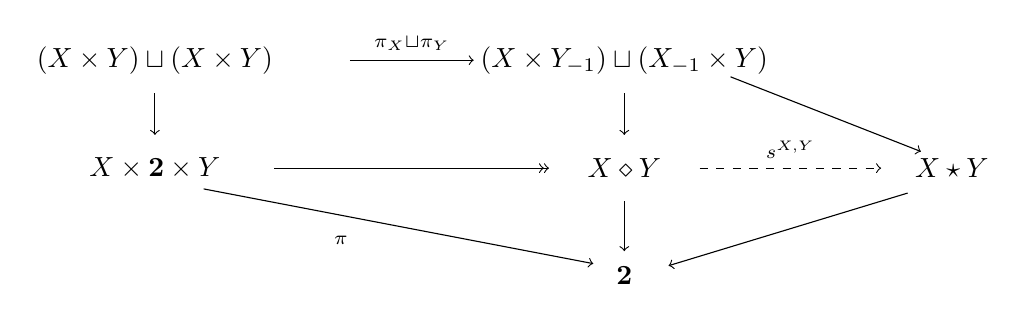
\begin{tikzpicture}[x=1.6em,y=1.5em]
  \node (tl) at (0,2.6) {$(X\times Y)\sqcup(X\times Y)$};
  \node (tr) at (10.6,2.6) {$(X\times Y_{-1})\sqcup(X_{-1}\times Y)$};
  \node (ml) at (0,0) {$X\times\qcTwo\times Y$};
  \node (mm) at (10.6,0) {$X\diamond Y$};
  \node (mr) at (18.0,0) {$X\star Y$};
  \draw[->] (4.4,2.6) -- node[above]{$\scriptstyle\pi_{X}\sqcup\pi_{Y}$} (7.2,2.6);
  \draw[->] (0,1.8) -- (0,0.8);
  \draw[->] (10.6,1.8) -- (10.6,0.8);
  \draw[->] (13.0,2.2) -- (17.3,0.4);
  \draw[->>] (2.7,0) -- (8.9,0);
  \draw[->,dashed] (12.3,0) -- node[above]{$\scriptstyle s^{X,Y}$} (16.4,0);
  \node at (9.2,0.6) {$\scriptstyle\ulcorner$};
  \node (two) at (10.6,-2.6) {$\mathbf{2}$};
  \draw[->] (1.1,-0.5) -- (9.9,-2.3);
  \node at (4.2,-1.75) {$\scriptstyle\pi$};
  \draw[->] (10.6,-0.8) -- (10.6,-2.0);
  \draw[->] (17.0,-0.6) -- (11.6,-2.35);
\end{tikzpicture}
\end{rveq}
注意 $X\diamond Y$ 与 $X\star Y$ 在 $\mathbf{2}$ 的两个端点 $0,1$ 之上的%
诸\trFiber{}分别为 $X\times Y_{-1}$ 与 $X_{-1}\times Y$，且映射 $s^{X,Y}$%
与这些\trFiber{}的包含相交换。

映射 $s^{X,Y}$ 定义在 $X\diamond Y$ 的那些映满 $\mathbf{2}$ 的 $n$-单纯形%
之上：它把代表 $X\diamond Y$ 的一个 $n$-单纯形的三元组%
$(\sigma\in X_{n},\ \alpha\colon[n]\to[1],\ \tau\in Y_{n})$ 送到代表%
$X\star Y$ 的一个 $n$-单纯形的二元组
$(\sigma|_{[0,\dots,k]}\in X_{k},\ \tau|_{[k+1,\dots,n]}\in Y_{n-k-1})$，
其中 $k\in[n]$ 是 $\alpha^{-1}(0)$ 中的最大顶点。
\end{proof}

我们现在证明：诸单纯形的\trFatJoin{}与诸单纯形的\trJoin{}之间的自然比较，定义了%
带标记\trHomotopyEquivalence{}的一个分支（见\cref{def:marked-homotopy}）。
\begin{proposition}\label{prop:comparison-marked-homotopy-retract}
\emph{对每一对 $n,m\ge-1$，增广单纯集的映射
\begin{equation*}
s^{n,m}\colon\Delta[n]\diamond\Delta[m]\longrightarrow\Delta[n]\star\Delta[m]
\qquad\in\sSet_{+}^{\Delta_{+}\times\Delta_{+}}
\end{equation*}
是一个带标记\trHomotopy{}\trRetract{}等价，并且在 $n=-1$ 或 $m=-1$ 的情形下
是一个\trIsomorphism}。
\end{proposition}

\begin{proof}
为定义 $s^{n,m}$ 的一个\trSection{}与左\trHomotopy{}逆，我们考虑一个由其在
顶点上的保序作用所确定的映射：
\begin{equation*}
\begin{aligned}
\Delta[n+1+m]\;&\xrightarrow{\ t^{n,m}\ }\;\Delta[n]\times\Delta[1]\times\Delta[m]\\
i&\;\longmapsto\;
\begin{cases}
(i,0,0) & \text{若 } i\le n,\\
(n,1,i-n-1) & \text{若 } i>n.
\end{cases}
\end{aligned}
\end{equation*}
并立即可注意到 $\bar{s}^{n,m}\bar{t}^{n,m}=\mathrm{id}$。反向的复合则由显式公式%
给出：
\begin{equation*}
\begin{aligned}
\Delta[n]\times\Delta[1]\times\Delta[m]\;&\xrightarrow{\ \bar{t}^{n,m}\bar{s}^{n,m}\ }\;\Delta[n]\times\Delta[1]\times\Delta[m]\\
(i,0,k)&\;\longmapsto\;(i,0,0)\\
(i,1,k)&\;\longmapsto\;(n,1,k)\mbox{.}
\end{aligned}
\end{equation*}
现在我们可以定义 $[n]\times[1]\times[m]$ 上的一个相关的保序自映射%
$\bar{u}^{n,m}$：
\begin{equation*}
\begin{aligned}
\Delta[n]\times\Delta[1]\times\Delta[m]\;&\xrightarrow{\ \bar{u}^{n,m}\ }\;\Delta[n]\times\Delta[1]\times\Delta[m]\\
(i,0,k)&\;\longmapsto\;(i,0,0)\\
(i,1,k)&\;\longmapsto\;(i,1,k)
\end{aligned}
\end{equation*}
这之所以引人关注，是因为在此类映射的逐点序之下我们有
$\bar{u}^{n,m}\le\bar{t}^{n,m}\circ\bar{s}^{n,m}$ 且
$\bar{u}^{n,m}\le\mathrm{id}_{[n]\times[1]\times[m]}$，它们代表诸单纯%
\trHomotopy：
\begin{center}
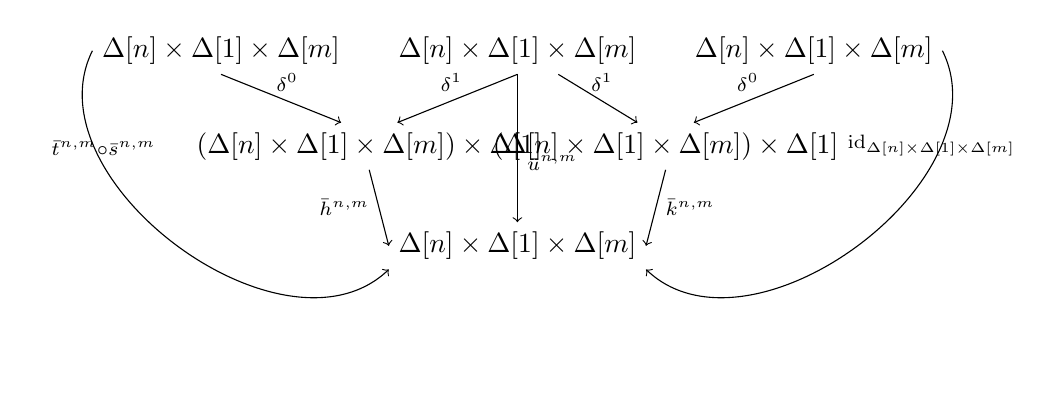
\begin{tikzpicture}[x=1.05em,y=1.5em]
  \node (A) at (0,3.4) {$\Delta[n]\times\Delta[1]\times\Delta[m]$};
  \node (B) at (10.2,3.4) {$\Delta[n]\times\Delta[1]\times\Delta[m]$};
  \node (C) at (20.4,3.4) {$\Delta[n]\times\Delta[1]\times\Delta[m]$};
  \node (L) at (5.1,1.1) {$(\Delta[n]\times\Delta[1]\times\Delta[m])\times\Delta[1]$};
  \node (R) at (15.3,1.1) {$(\Delta[n]\times\Delta[1]\times\Delta[m])\times\Delta[1]$};
  \node (D) at (10.2,-1.3) {$\Delta[n]\times\Delta[1]\times\Delta[m]$};
  \draw[->] (A.south) -- node[above,pos=0.55]{$\scriptstyle\delta^{0}$} (L.140);
  \draw[->] (B.south) -- node[above,pos=0.55]{$\scriptstyle\delta^{1}$} (L.40);
  \draw[->] (B.330) -- node[above,pos=0.55]{$\scriptstyle\delta^{1}$} (R.140);
  \draw[->] (C.south) -- node[above,pos=0.55]{$\scriptstyle\delta^{0}$} (R.40);
  \draw[->] (B.south) -- node[right,pos=0.6]{$\scriptstyle\bar{u}^{n,m}$} (D.north);
  \draw[->] (L.south) -- node[left,pos=0.5]{$\scriptstyle\bar{h}^{n,m}$} (D.west);
  \draw[->] (R.south) -- node[right,pos=0.5]{$\scriptstyle\bar{k}^{n,m}$} (D.east);
  \draw[->] (A.west) to[bend right=80] node[above,pos=0.28]{$\scriptstyle\bar{t}^{n,m}\circ\bar{s}^{n,m}$} (D.south west);
  \draw[->] (C.east) to[bend left=80] node[above,pos=0.28]{$\scriptstyle\mathrm{id}_{\Delta[n]\times\Delta[1]\times\Delta[m]}$} (D.south east);
\end{tikzpicture}
\end{center}

沿\cref{def:fat-join-augmented}所定义的同余作商，这就诱导出单纯映射%
$t^{n,m}\colon\Delta[n]\star\Delta[m]\to\Delta[n]\diamond\Delta[m]$ 与%
$u^{n,m}\colon\Delta[n]\diamond\Delta[m]\to\Delta[n]\diamond\Delta[m]$，%
使得 $s^{n,m}t^{n,m}=\mathrm{id}_{\Delta[n]\star\Delta[m]}$，以及单纯%
\trHomotopy{} $h^{n,m}$ 与 $k^{n,m}$，它们组装成如下图式：
\begin{center}
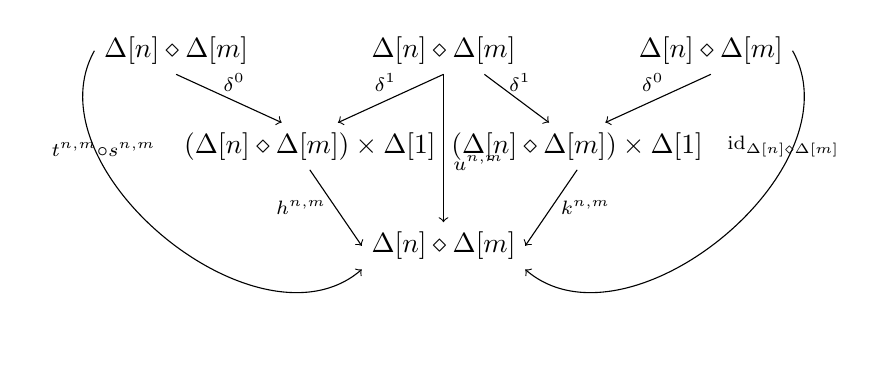
\begin{tikzpicture}[x=1.15em,y=1.5em]
  \node (A) at (0,3.4) {$\Delta[n]\diamond\Delta[m]$};
  \node (B) at (8.4,3.4) {$\Delta[n]\diamond\Delta[m]$};
  \node (C) at (16.8,3.4) {$\Delta[n]\diamond\Delta[m]$};
  \node (L) at (4.2,1.1) {$(\Delta[n]\diamond\Delta[m])\times\Delta[1]$};
  \node (R) at (12.6,1.1) {$(\Delta[n]\diamond\Delta[m])\times\Delta[1]$};
  \node (D) at (8.4,-1.3) {$\Delta[n]\diamond\Delta[m]$};
  \draw[->] (A.south) -- node[above,pos=0.55]{$\scriptstyle\delta^{0}$} (L.140);
  \draw[->] (B.south) -- node[above,pos=0.55]{$\scriptstyle\delta^{1}$} (L.40);
  \draw[->] (B.330) -- node[above,pos=0.55]{$\scriptstyle\delta^{1}$} (R.140);
  \draw[->] (C.south) -- node[above,pos=0.55]{$\scriptstyle\delta^{0}$} (R.40);
  \draw[->] (B.south) -- node[right,pos=0.6]{$\scriptstyle u^{n,m}$} (D.north);
  \draw[->] (L.south) -- node[left,pos=0.5]{$\scriptstyle h^{n,m}$} (D.west);
  \draw[->] (R.south) -- node[right,pos=0.5]{$\scriptstyle k^{n,m}$} (D.east);
  \draw[->] (A.west) to[bend right=80] node[above,pos=0.3]{$\scriptstyle t^{n,m}\circ s^{n,m}$} (D.south west);
  \draw[->] (C.east) to[bend left=80] node[above,pos=0.3]{$\scriptstyle\mathrm{id}_{\Delta[n]\diamond\Delta[m]}$} (D.south east);
\end{tikzpicture}
\end{center}

为看出映射 $h^{n,m}$ 与 $k^{n,m}$ 确实定义带标记\trHomotopy，\cref{def:marked-homotopy}
告诉我们：必须验证，对 $\Delta[n]\diamond\Delta[m]$ 的每个 $0$-单纯形%
$[i,j,k]_{\sim}$，$(\Delta[n]\diamond\Delta[m])\times\Delta[1]$ 的%
$1$-单纯形 $([i,j,k]_{\sim}\cdot\sigma^{0},\ \mathrm{id}_{[1]})$ 在%
$h^{n,m}$ 与 $k^{n,m}$ 之下被映到 $\Delta[n]\diamond\Delta[m]$ 中退化的、%
因而是带标记的单纯形。我们对指标 $j$ 分情形论证。若 $j=0$，则
$\bar{u}^{n,m}(i,0,k)=(i,0,0)=\bar{t}^{n,m}\bar{s}^{n,m}(i,0,k)$，且%
$(i,0,0)\sim(i,0,k)=\mathrm{id}(i,0,k)$，故 $h^{n,m}$ 与 $k^{n,m}$ 二者的%
分量都是退化的。
\footnote{原书印作「$(i,0,0)\sim(i,0,k)=\bar{t}^{n,m}\circ\bar{s}^{n,m}(i,0,k)$」；
按上文所列公式 $\bar{s}^{n,m}(i,0,k)=i$ 与 $\bar{t}^{n,m}(i)=(i,0,0)$，%
末端 $\bar{t}^{n,m}\bar{s}^{n,m}(i,0,k)=(i,0,0)$，疑为末端映射之名误植，%
此处径改。——译者注}
若 $j=1$，则
$\bar{u}^{n,m}(i,1,k)=(i,1,k)\sim(n,1,k)=\bar{t}^{n,m}\bar{s}^{n,m}(i,1,k)$%
\yizhu{原书此处中间项印作「$(n,i,k)$」；按上文所列公式
$\bar{t}^{n,m}\bar{s}^{n,m}(i,1,k)=(n,1,k)$，疑为中间项误植，此处径改。%
——译者注}，%
故 $h^{n,m}$ 与 $k^{n,m}$ 的分量同样都是退化的。
于是，$s^{n,m}$ 扩张成一个带标记\trHomotopy{}\trRetract{}等价，其等价逆为%
$t^{n,m}$。
\end{proof}

\cref{prop:comparison-marked-homotopy-retract}的带标记单纯%
\trHomotopyEquivalence{}见证了\cref{lem:fat-join-comparison}中所考虑的%
$\sSet_{+}^{\Delta_{+}\times\Delta_{+}}$里两个\trDiagram{}之间的、某种合适
意义下的逐点\trWeakEquivalence。这是下述证明的关键原料：增广单纯集的典范
映射 $s^{X,Y}\colon X\diamond Y\to X\star Y$ 在某种合适的意义下也是%
\trWeakEquivalence；但这一结论要求我们先探究带标记单纯集的\trHomotopy{}论
与\trQuasiCategory{}的\trHomotopy{}论之间的联系。我们将在 D.4 节中建立这一
联系，并在 D.6 节中重续这条论证线索。

我们以最后一个结果来结束本节，它是\cref{lem:leibniz-join-horn-boundary}%
的一个带标记类比。\cref{def:join-simplicial-sets}的\trJoin{}构造在\cite{bib128}
中被扩张到\trMarkedSimplicialSet。

\begin{definition}[\trMarkedSimplicialSet{}的\trJoin]\label{def:join-marked-simplicial-sets}
\trSimplicial\trJoin{}提升为一个\trJoin\trBifunctor
\begin{equation*}
\sSet^{+}\times\sSet^{+}\xrightarrow{\ \star\ }\sSet^{+}
\end{equation*}
其中，形如 $(\alpha,\beta)\colon\Delta[n]\to A\star B$ 的单纯形——其分量%
为 $\alpha\colon\Delta[k]\to A$ 与 $\beta\colon\Delta[n-k-1]\to B$——在%
$A\star B$ 中被标记，当且仅当 $\alpha$ 或 $\beta$ 至少一者在 $A$ 或 $B$ 中%
被标记。
\end{definition}

\begin{lemma}\label{lem:leibniz-join-complicial}
\begin{enumerate}[label=(\roman*)]
\item \emph{一个复状号角扩张与一个\trBoundary{}包含的 Leibniz \trJoin%
\trIsomorphism{}于单个复状号角扩张：}
\begin{equation*}
(\Lambda^{k}[n]\hookrightarrow_{r}\Delta^{k}[n])\mathbin{\hat{\star}}
(\partial\Delta[m]\hookrightarrow_{r}\Delta[m])
\cong
\Lambda^{k}[n+1+m]\hookrightarrow_{r}\Delta^{k}[n+1+m]
\end{equation*}
\emph{除非 $k=n$，此时
$(\Lambda^{n}[n]\hookrightarrow_{r}\Delta^{n}[n])\mathbin{\hat{\star}} (\partial\Delta[m]\hookrightarrow_{r}\Delta[m])$
是 $\Lambda^{n}[n+1+m]\hookrightarrow_{r}\Delta^{n}[n+1+m]$ 的一个%
\trPushout。}
\item \emph{下列诸 Leibniz \trJoin{}是复状薄性扩张}
\begin{gather*}
(\Delta^{k}[n]'\hookrightarrow_{e}\Delta^{k}[n]'')\mathbin{\hat{\star}}
(\Delta[m]\hookrightarrow_{e}\Delta[m]_{t})
\cong
\Delta^{k}[n+1+m]'\hookrightarrow_{e}\Delta^{k}[n+1+m]''\\
(\Delta^{k}[n]'\hookrightarrow_{e}\Delta^{k}[n]'')\mathbin{\hat{\star}}
(\partial\Delta[m]\hookrightarrow_{r}\Delta[m])
\cong
\Delta^{k}[n+1+m]'\hookrightarrow_{e}\Delta^{k}[n+1+m]''
\end{gather*}
\emph{除非 $k=n$，此时诸 Leibniz \trJoin{}反而是
$\Delta^{k}[n+1+m]'\hookrightarrow_{e}\Delta^{k}[n+1+m]''$ 的%
\trPushout，而
$(\Delta^{k}[n]'\hookrightarrow_{e}\Delta^{k}[n]'')\mathbin{\hat{\star}} (\Delta[m]\hookrightarrow_{e}\Delta[m]_{t})$
则是恒同映射。}
\end{enumerate}
\end{lemma}

由于\trJoin{}是反对称的——有
$(A\star B)^{\mathrm{op}}\cong B^{\mathrm{op}}\star A^{\mathrm{op}}$——
把每个 Leibniz \trJoin{}的左、右两映射相互交换而得的那些情形，都容易从这里所%
考虑的情形推得。

\begin{proof}
(i) 中作为单纯集的底映射已在\cref{lem:leibniz-join-horn-boundary}中被%
辨识，故只剩下考虑诸标记。类似地，在 (ii) 中所考虑的三个 Leibniz \trJoin{}的%
每一个里，作为单纯集的底映射都是一个\trMonomorphism{}与一个恒同的%
Leibniz \trJoin，从而是一个恒同，故只剩下考虑所得\trEntireInclusion{}中的诸标记。由于%
\trMarkedSimplicialSet{}之\trJoin{}中的一个单纯形被标记，当且仅当它的分量之一
被标记，这一描述颇便于分情形论证。我们把细节留给%
\cref{ex:finish-complicial-join-proof}或文献\cite{bib129,bib38}。
\end{proof}

\cref{def:slices-of-simplicial-sets}的切片构造也扩张到\trMarkedSimplicialSet。
我们为这一构造采用新的记号，这是因为：带标记\trJoin{}的底单纯集通常并不是底
单纯集之相应映射的切片。

\begin{lemma}\label{lem:marked-slices}
\emph{对\trMarkedSimplicialSet{}的任何映射 $f\colon X\to A$，存在由如下%
\trUniversalProperty{}刻画的\trMarkedSimplicialSet{} ${}^{f/\!/}\!A$ 与%
$A_{/\!/f}$：}
\begin{equation*}
\left\{\vcenter{\hbox{\begin{tikzpicture}[x=1.2em,y=1.2em]
  \node (x) at (1.4,0.9) {$X$};
  \node (a) at (4.2,0) {$A$};
  \node (xy) at (0,-0.9) {$X\star Y$};
  \draw[->] (2.2,0.78) -- (3.8,0.25);
  \node at (3.3,0.75) {$\scriptstyle f$};
  \draw[right hook->] (1.0,0.4) -- (0.4,-0.5);
  \draw[->] (1.2,-0.9) -- (3.2,-0.35);
\end{tikzpicture}}}\right\}
\cong
\left\{\,Y\to{}^{f/\!/}\!A\,\right\}
\qquad
\left\{\vcenter{\hbox{\begin{tikzpicture}[x=1.2em,y=1.2em]
  \node (x) at (1.4,0.9) {$X$};
  \node (a) at (4.2,0) {$A$};
  \node (xy) at (0,-0.9) {$Y\star X$};
  \draw[->] (2.2,0.78) -- (3.8,0.25);
  \node at (3.3,0.75) {$\scriptstyle f$};
  \draw[right hook->] (1.0,0.4) -- (0.4,-0.5);
  \draw[->] (1.2,-0.9) -- (3.2,-0.35);
\end{tikzpicture}}}\right\}
\cong
\left\{\,Y\to A_{/\!/f}\,\right\}\mbox{.}
\end{equation*}
\end{lemma}

\begin{proof}
\cref{ex:marked-slices-proof}。
\end{proof}

\subsection*{练习}

\begin{exercise}\label{ex:components-decomposition-exercise}
证明\cref{lem:components-decomposition}。
\end{exercise}

\begin{exercise}[{\cite{bib129,bib38}}]\label{ex:finish-complicial-join-proof}
完成\cref{lem:leibniz-join-complicial}的证明。
\end{exercise}

\begin{exercise}\label{ex:entire-inclusions-identity}
通过证明两个\trEntireInclusion{}的 Leibniz \trJoin{}是一个恒同，推广%
\cref{lem:leibniz-join-complicial}(ii)的最后一种情形。
\end{exercise}

\begin{exercise}\label{ex:marked-slices-proof}
证明\cref{lem:marked-slices}。
\end{exercise}
   %

\section{笛卡尔积的 Leibniz 稳定性}\label{sec:leibniz-stability-cartesian-products}

现在我们把注意力转向相对于\trCartesianProduct{}定义的类似 Leibniz 构造——
在\trMarkedSimplicialSet{}的语境中，它在 \cite{bib129} 中被称作\emph{Gray
张量积}（Gray tensor product）。我们先以一个关于\trLeibnizProduct{}之几何的基础
结果作为热身。

\begin{lemma}\label{lem:leibniz-product-mono}
\trSimplicialSet{}的任意一对\trMonomorphism{}的\trLeibnizProduct{}是一个%
\trMonomorphism。
\end{lemma}

\begin{proof}
诸\trProduct、诸\trPushout{}与诸\trMonomorphism{}都是在集合的\trCategory{}%
中逐点确定的，故此结果由下述事实得出：对集合的\trMonomorphism{}
$S\hookrightarrow T$ 与 $U\hookrightarrow V$，\trLeibnizProduct
\[ (S\hookrightarrow T)\mathbin{\widehat{\times}}(U\hookrightarrow V)
   \cong\bigl(S\times V\underset{S\times U}{\cup}T\times U
   \hookrightarrow T\times V\bigr) \]
是一个\trMonomorphism——逐一检视即明。
\end{proof}

\begin{remark}[为何称作「Leibniz」]\label{rem:why-leibniz}
由一对\trSimplex{}\trBoundary{}包含的\trLeibnizProduct{}所定义的包含
\begin{multline*}
(\partial\Delta[n]\hookrightarrow\Delta[n])\mathbin{\widehat{\times}}
(\partial\Delta[m]\hookrightarrow\Delta[m])\cong\\
\partial\Delta[n]\times\Delta[m]
\underset{\partial\Delta[n]\times\partial\Delta[m]}{\cup}
\Delta[n]\times\partial\Delta[m]\hookrightarrow\Delta[n]\times\Delta[m]
\end{multline*}
在几何上对应于\trPrism{}的\trBoundary{}
$\partial(\Delta[n]\times\Delta[m])\hookrightarrow\Delta[n]\times\Delta[m]$
这一包含。而等同
\[ \partial(\Delta[n]\times\Delta[m])\cong
   \partial\Delta[n]\times\Delta[m]
   \underset{\partial\Delta[n]\times\partial\Delta[m]}{\cup}
   \Delta[n]\times\partial\Delta[m] \]
在形式上类似于通常称作「Leibniz 法则」的种种恒等式。
\end{remark}

为证明一个关于\trMarkedSimplicialSet{}的类似结果，我们首先需要下述观察：

\begin{proposition}\label{prop:marked-cartesian-closed}
\trMarkedSimplicialSet{}的\trCategory{}是\trCartesianClosed，其中
\begin{itemize}
\item \trCartesianProduct{}定义如下：底\trSimplicialSet{}的%
  \trCartesianProduct{}中的一个\trSimplex{}被标记，当且仅当它的两个分量
  都是带标记\trSimplex；
\item \trInternalHom{} $Y^{X}$ 定义为这样一个\trSimplicialSet：其诸
  $n$-\trSimplex{}是\trMarkedSimplicialSet{}的映射
  $\sigma\colon X\times\Delta[n]\to Y$，而 $\sigma$ 被标记，当且仅当该
  映射可\trExtension{}为一个\trMarkedSimplicialSet{}的映射：
\begin{center}
\begin{tikzpicture}[x=1.8em,y=1.5em]
  \node (xt) at (0,1.3) {$X\times\Delta[n]$};
  \node (y) at (4.4,1.3) {$Y$};
  \node (xe) at (0,-1.1) {$X\times\Delta[n]_{t}$};
  \draw[->] (xt) -- node[above]{$\scriptstyle\sigma$} (y);
  \draw[right hook->] (xe) -- node[left]{$\scriptstyle e$} (xt);
  \draw[->,dashed] (1.1,-0.85) -- (3.7,0.95);
  \node at (2.2,0.25) {$\scriptstyle\sigma$};
\end{tikzpicture}
\end{center}
\end{itemize}
\end{proposition}

\begin{proof}
由\trProduct{}的\trUniversalProperty{}及其封闭性，显然：若这些对象存在，
\trCartesianProduct{}与\trInternalHom{}就必定以这种方式来定义。为验证这一%
\trAdjunction，回顾\cref{prop:reflective-embedding}：\trMarkedSimplicialSet{}%
作为反射全子范畴嵌入预层\trCategory{}
$\mathcal{S}et^{t\Delta^{\mathrm{op}}}$ 之中。由附录 A 中的%
\cref{exa:cartesian-closed-examples}，\trCategory{}
$\mathcal{S}et^{t\Delta^{\mathrm{op}}}$ 是\trCartesianClosed，而且这一
嵌入保持刚才定义的诸\trProduct{}与诸\trInternalHom{}。于是我们得出结论：
把相应的自然\trIsomorphism{}从 $\mathcal{S}et^{t\Delta^{\mathrm{op}}}$
限制到其全子范畴上，这些数据便定义了 $\sSet^{+}$ 上一个双变量\trAdjunction{}%
的诸\trFunctor。
\end{proof}

\cref{lem:leibniz-product-mono}的结果可以扩张到带标记的语境。我们的证明用到
一条也在别处被调用的简单观察。

\begin{lemma}\label{lem:leibniz-entire}
\trMarkedSimplicialSet{}的任一映射与一个\trEntireInclusion{}的\trLeibnizProduct{}是一个\trEntireInclusion。
\end{lemma}

\begin{proof}
按定义，$f\colon X\to Y$ 与 $i\colon U\hookrightarrow_{e}V$ 的\trLeibnizProduct{}是
如下所诱导的\trMarkedSimplicialSet{}的映射
\begin{center}
\begin{tikzpicture}[x=1.8em,y=1.5em]
  \node (xu) at (0,1.9) {$X\times U$};
  \node (xv) at (3.6,1.9) {$X\times V$};
  \node (yu) at (0,0.2) {$Y\times U$};
  \fill (3.0,0.2) circle (1.1pt);
  \node at (2.62,0.55) {$\scriptstyle\ulcorner$};
  \node (yv) at (4.6,-1.7) {$Y\times V$};
  \draw[right hook->] (xu) -- node[above]{$\scriptstyle X\times i$} node[pos=0.2,below]{$\scriptstyle e$} (xv);
  \draw[->] (0,1.55) -- (0,0.6);
  \node at (-0.8,1.05) {$\scriptstyle f\times U$};
  \draw[->] (3.6,1.55) -- (3.05,0.55);
  \draw[->] (0.75,0.2) -- (2.55,0.2);
  \node at (1.65,-0.2) {$\scriptstyle\hookrightarrow_{e}$};
  \draw[->,dashed] (3.15,-0.1) -- (4.3,-1.35);
  \draw[->] (3.95,1.6) .. controls (5.5,0.9) and (5.6,-0.6) .. (5.15,-1.55);
  \node at (5.6,0.15) {$\scriptstyle f\times V$};
  \draw[->] (0.55,-0.15) .. controls (2.0,-1.15) and (3.4,-1.7) .. (3.9,-1.72);
  \node at (1.7,-1.2) {$\scriptstyle Y\times i$};
  \node at (4.05,-2.05) {$\scriptstyle\hookrightarrow_{e}$};
\end{tikzpicture}
\end{center}
注意\trForgetfulFunctor{} $(-)_{0}\colon\sSet^{+}\to\sSet$ 保持诸%
\trProduct{}与诸\trPushout，并回顾：\trMarkedSimplicialSet{}的一个映射是%
\trEntireInclusion，当且仅当其底映射是一个\trIsomorphism。由于一个\trSimplicialSet{}%
与一个\trIsomorphism{}的\trProduct{}是\trIsomorphism，映射
$X\times U\hookrightarrow_{e}X\times V$ 与
$Y\times U\hookrightarrow_{e}Y\times V$ 都是\trEntireInclusion。又由于诸%
\trIsomorphism{}的\trPushout{}是\trIsomorphism，剩下那条水平映射也是%
\trEntireInclusion。最后，由于诸\trIsomorphism{}满足\trTwoOfThreeProperty，\trLeibnizProduct
映射必定也是\trEntireInclusion。
\end{proof}

\begin{lemma}\label{lem:leibniz-regular}
两个正则包含的\trLeibnizProduct{}仍是正则包含。
\end{lemma}

\begin{proof}
由\cref{lem:leibniz-product-mono}，两个正则包含
$A\hookrightarrow_{r}B$ 与 $C\hookrightarrow_{r}D$ 的\trLeibnizProduct{}之底%
\trSimplicialSet{}是\trMonomorphism
\[ A\times D\underset{A\times C}{\cup}B\times C
   \hookrightarrow B\times D\mbox{.} \]
特别地，注意分量 $A\times D$ 与 $B\times C$ 的诸包含联合满地映到该映射的
定义域上。我们的任务是证明：$A\times D\underset{A\times C}{\cup}B\times C$
中任何一个在 $B\times D$ 中被标记的 $n$-\trSimplex{}，在
$A\times D\underset{A\times C}{\cup}B\times C$ 中也被标记。我们分情形
论证，并不失一般性假设该 $n$-\trSimplex{}位于来自 $B\times C$ 的包含的像
之中。此时，映射 $B\times C\hookrightarrow_{r}B\times D$ 的正则性蕴含：
它在 $A\times D\underset{A\times C}{\cup}B\times C$ 中被标记，正如所断言。
\end{proof}

\trMarkedSimplicialSet{}的一个一般\trMonomorphism{}既非正则包含亦非\trEntireInclusion，
但\trMarkedSimplicialSet{}的诸生成\trMonomorphism{}却具有这两种性质之一。
于是，由\cref{lem:leibniz-entire}与\cref{lem:leibniz-regular}，我们立即
得出：

\begin{lemma}\label{lem:leibniz-generating}
对任意 $n,m\ge 0$，诸\trLeibnizProduct
\begin{gather*}
(\partial\Delta[n]\hookrightarrow_{r}\Delta[n])\mathbin{\widehat{\times}}
(\partial\Delta[m]\hookrightarrow_{r}\Delta[m]),\qquad
(\partial\Delta[n]\hookrightarrow_{r}\Delta[n])\mathbin{\widehat{\times}}
(\Delta[m]\hookrightarrow_{e}\Delta[m]_{t}),\\
\text{以及}\qquad
(\Delta[n]\hookrightarrow_{e}\Delta[n]_{t})\mathbin{\widehat{\times}}
(\Delta[m]\hookrightarrow_{e}\Delta[m]_{t})
\end{gather*}
都是\trMarkedSimplicialSet{}的\trMonomorphism。
\end{lemma}

作为一个推论，我们可以借助一个在本章中反复出现的十分一般的论证来刻画%
\trMarkedSimplicialSet{}的任意\trMonomorphism{}的\trLeibnizProduct。

\begin{corollary}\label{cor:leibniz-mono-tf}
\begin{enumerate}[label=(\roman*)]
\item \trMarkedSimplicialSet{}的任意一对\trMonomorphism{}的\trLeibnizProduct{}仍是
  一个\trMonomorphism。
\item \trMarkedSimplicialSet{}的任一\trTrivialFibration{}与任一%
  \trMonomorphism{}的 Leibniz 指数（Leibniz exponential）仍是一个%
  \trTrivialFibration。
\end{enumerate}
\end{corollary}

\begin{proof}
以\cref{lem:leibniz-two-variable-adjunction}的术语来说，这两条陈述合起来
断言：由\trCartesianProduct{}与\trInternalHom{}定义的双变量\trAdjunction{}%
相对于（\trMonomorphism，\trTrivialFibration）这一%
\trWeakFactorizationSystem{}是一个 Leibniz 双变量\trAdjunction。由
\cref{rem:leibniz-generators}，这可由
\cref{lem:mono-marked-cellularly-generated}与\cref{lem:leibniz-generating}
所建立的性质得出。
\end{proof}

困难得多的是证明：带标记\trAnodyneExtension{}类对于带标记\trMonomorphism{}类具有
Leibniz 稳定性。我们证明一个略更具体的结果，它同时刻画了内、左或右带标记%
\trAnodyneExtension{}的情形——这些情形分别把不等式 $0\le k\le n$ 限制为 $0<k<n$、
$k<n$ 或 $0<k$。

\begin{proposition}\label{prop:leibniz-marked-anodyne}
对 $n\ge 1$、$m\ge 0$ 且 $0<k\le n$，下列\trLeibnizProduct{}中的每一个都是右带标记%
\trAnodyneExtension，并且当 $k<n$ 时是内带标记\trAnodyneExtension：
\begin{gather*}
(\Lambda^{k}[n]\hookrightarrow_{r}\Delta^{k}[n])\mathbin{\widehat{\times}}
(\partial\Delta[m]\hookrightarrow_{r}\Delta[m])\\
(\Lambda^{k}[n]\hookrightarrow_{r}\Delta^{k}[n])\mathbin{\widehat{\times}}
(\Delta[m]\hookrightarrow_{e}\Delta[m]_{t})\\
(\Delta^{k}[n]'\hookrightarrow_{e}\Delta^{k}[n]'')\mathbin{\widehat{\times}}
(\partial\Delta[m]\hookrightarrow_{r}\Delta[m])\\
(\Delta^{k}[n]'\hookrightarrow_{e}\Delta^{k}[n]'')\mathbin{\widehat{\times}}
(\Delta[m]\hookrightarrow_{e}\Delta[m]_{t})
\end{gather*}
\end{proposition}

鉴于\trCartesianProduct{}的对称性，\trHorn{}包含与\trSimplex{}\trBoundary{}%
包含何者居左、何者居右并无分别。这一结果的证明需要某些特殊记号来描述%
\trSimplex{}的\trCartesianProduct。

\begin{digression}[论洗牌]\label{dig:on-shuffles}
由于 $\Delta[n]$ 是偏序集（poset）$[n]$ 的\trNerve，一个 $r$-\trSimplex{}
$i\colon\Delta[r]\to\Delta[n]$ 同样可以由出现于其像中的顶点的有序序列
$i_{0}\le\cdots\le i_{r}\in[n]$ 来编码。

由\trProduct{}的\trUniversalProperty，$\Delta[n]\times\Delta[m]$ 中的一个
$r$-\trSimplex{}由一个 $r$-\trSimplex{} $i\colon\Delta[r]\to\Delta[n]$ 与一个
$r$-\trSimplex{} $j\colon\Delta[r]\to\Delta[m]$ 给出。由于
$\Delta[n]\times\Delta[m]$ 是偏序集 $[n]\times[m]$ 的\trNerve，这样的%
\trSimplex{}与由二元组构成的有序序列
\begin{rveq}\label{eq:pair-sequence}
(i_{0},j_{0})\le(i_{1},j_{1})\le\cdots\le(i_{r},j_{r})
\end{rveq}
一一对应，其中每个 $i_{s}\in[n]$、每个 $j_{t}\in[m]$；而且它退化，当且仅当
这些不等式中的某一个是等式。

\trSimplicialSet{} $\Delta[n]\times\Delta[m]$ 的非退化
$(n+m)$-\trSimplex{}称作\textbf{洗牌}（shuffles）；它们是具有最高维数的%
\trSimplex。一个 $(n+m)$-\trSimplex{} $(i,j)$ 定义一个洗牌，当且仅当对一切
$t\in[n+m]$ 都有 $i_{t}+j_{t}=t$。若把 $[n]\times[m]$ 的对象排布成一个
矩形网格，洗牌便是那些从 $(0,0)$ 出发、以 $(n,m)$ 收尾的极大长度非退化
路径——每一步恰给某一个坐标加一。
\end{digression}

下面证明的第一个情形，是把 Dugger 与 Spivak 的一个论证 \cite[A.1]{bib36}
改编到带标记的语境。

\begin{proof}[\cref{prop:leibniz-marked-anodyne}的证明]
由\cref{lem:leibniz-regular}，\trLeibnizProduct{}
$(\Lambda^{k}[n]\hookrightarrow_{r}\Delta^{k}[n])\mathbin{\widehat{\times}}(\partial\Delta[m]\hookrightarrow_{r}\Delta[m])$ 是正则包含
\[ \Lambda^{k}[n]\times\Delta[m]
   \underset{\Lambda^{k}[n]\times\partial\Delta[m]}{\cup}
   \Delta^{k}[n]\times\partial\Delta[m]
   \hookrightarrow_{r}\Delta^{k}[n]\times\Delta[m]\mbox{.} \]
一个非退化 $r$-\trSimplex{} \eqref{eq:pair-sequence} 于
$\Delta^{k}[n]\times\Delta[m]$ 中不在这个\trLeibnizProduct{}包含的定义域内，当且仅当%
\yizhu{原书于此印作「of $\Lambda^{k}[n]\times\Delta[m]$」，然该并集之定义域
本就包含 $\Lambda^{k}[n]\times\Delta[m]$，其中的\trSimplex{}无从「缺失」；
按文义应为余域 $\Delta^{k}[n]\times\Delta[m]$ 之误，此处径改。——译者注}
\begin{itemize}
\item 它的分量 $\{i_{0},\dots,i_{r}\}\supseteq[n]\setminus\{k\}$，并且
\item 它的分量 $\{j_{0},\dots,j_{r}\}\supseteq[m]$。
\end{itemize}
我们将这一包含过滤成一列正则包含
\[ \Lambda^{k}[n]\times\Delta[m]
   \underset{\Lambda^{k}[n]\times\partial\Delta[m]}{\cup}
   \Delta^{k}[n]\times\partial\Delta[m]=:Y^{-1}
   \hookrightarrow_{r}\cdots\hookrightarrow_{r}Y^{m}
   =\Delta^{k}[n]\times\Delta[m] \]
并论证：视情形而定，每个 $Y^{t}\hookrightarrow Y^{t+1}$ 都是右或内带标记%
\trAnodyne{}的。

从 $Y^{-1}:=\Lambda^{k}[n]\times\Delta[m]\underset{\Lambda^{k}[n]\times\partial\Delta[m]}{\cup}\Delta^{k}[n]\times\partial\Delta[m]$ 出发，我们把 $Y^{t}$ 定义为
$\Delta^{k}[n]\times\Delta[m]$ 的这样一个最小的正则单纯子集：它包含
$Y^{t-1}$ 以及每一个含有顶点 $(k,t)$ 的\trSimplex{}
\eqref{eq:pair-sequence}。由于每一个缺失的\trSimplex{}都是含有顶点
$(k,0),\dots,(k,m)$ 之一的某个\trSimplex{}的一个面，从此描述即清楚可见
$Y^{m}=\Delta^{k}[n]\times\Delta[m]$。

剩下的只是分析诸正则包含 $Y^{t-1}\hookrightarrow_{r}Y^{t}$，我们通过给出
另一重过滤来做到这一点：
\[ Y^{t-1}=Y^{t,n-1}\hookrightarrow_{r}Y^{t,n}\hookrightarrow_{r}
   \cdots\hookrightarrow_{r}Y^{t,n+m}=Y^{t}\mbox{.} \]

注意：$\Delta^{k}[n]\times\Delta[m]$ 中含有顶点 $(k,t)$ 且维数不超过 $n-1$
的\trSimplex{}都含于 $Y^{-1}$，因此那些含有顶点 $(k,t)$、附着到 $Y^{t-1}$
上以构成 $Y^{t}$ 的\trSimplex{}，其维数介于 $n$ 与 $n+m$ 之间。有鉴于此，
我们把 $Y^{t,r}$ 定义为 $\Delta^{k}[n]\times\Delta[m]$ 的包含 $Y^{t,r-1}$
与一切含有顶点 $(k,t)$ 的 $r$ 维\trSimplex{}的最小正则单纯子集。特别地，
$Y^{t,n-1}=Y^{t-1}$ 而 $Y^{t,n+m}=Y^{t}$。

我们现在论证：这一过滤中的每个正则包含都先是一个由诸复状号角扩张之余积
构成的推出，继而是诸复状薄性扩张之余积的推出
\begin{center}
\begin{tikzpicture}[x=1.9em,y=1.5em]
  \node (lam) at (0,2.6) {$\coprod_{\tau\in S^{t,r}}\Lambda^{\ell_{\tau}}[r]$};
  \node (ytr1) at (6.4,2.6) {$Y^{t,r-1}$};
  \node (dl) at (0,0) {$\coprod_{\tau\in S^{t,r}}\Delta^{\ell_{\tau}}[r]$};
  \fill (4.0,0) circle (1.1pt);
  \node at (3.62,0.35) {$\scriptstyle\lrcorner$};
  \node (dr) at (9.2,0) {$\coprod_{\tau\in T^{t,r}}\Delta^{\ell_{\tau}}[r]'$};
  \node (ytr) at (4.0,-2.6) {$Y^{t,r}$};
  \node (dd) at (9.2,-2.6) {$\coprod_{\tau\in T^{t,r}}\Delta^{\ell_{\tau}}[r]''$};
  \draw[->] (lam) -- (ytr1);
  \draw[right hook->] (0,2.1) -- node[left]{$\scriptstyle r$} (0,0.55);
  \draw[right hook->] (6.4,2.05) -- (4.15,0.4);
  \draw[->] (1.9,0) -- (3.6,0);
  \draw[->] (7.5,0) -- (4.4,0);
  \draw[right hook->] (9.2,0.55) -- node[right]{$\scriptstyle e$} (9.2,-2.05);
  \draw[right hook->] (4.0,-0.55) -- node[left]{$\scriptstyle e$} (4.0,-2.05);
  \node at (3.62,-2.2) {$\scriptstyle\lrcorner$};
  \draw[->] (7.5,-2.6) -- (4.8,-2.6);
\end{tikzpicture}
\end{center}
其由集合 $S^{t,r}$——含有顶点 $(k,t)$ 且尚未出现在 $Y^{t,r-1}$ 中的
$r$-\trSimplex{}之集——标引，而 $T^{t,r}\subset S^{t,r}$ 则定义为那些使
$\tau\delta^{\ell_{\tau}}$ 在 $\Delta^{k}[n]\times\Delta[m]$ 中被标记的
$r$-\trSimplex{} $\tau$ 组成的子集。此外，对每个 $\tau\in S^{t,r}$，我们将
看到 $0<\ell_{\tau}$，而当 $k<n$ 时 $\ell_{\tau}<r$。这将表明：该\trLeibnizProduct
是一个右带标记\trAnodyneExtension，并且当 $k<n$ 时是一个内带标记\trAnodyneExtension。

为看到这一点，设 $\tau\in S^{t,r}$ 是 $r$-\trSimplex{}
\[ (i_{0},j_{0})\le\cdots\le(i_{\ell_{\tau}},j_{\ell_{\tau}})=(k,t)
   \le\cdots\le(i_{r},j_{r}) \]
它以 $(k,t)$ 为其第 $\ell_{\tau}$ 个顶点；为便于阅读，下文将 $\ell_{\tau}$
写作 $\ell$。由于集合 $\{i_{0},\dots,i_{r}\}\supseteq[n]$ 且 $0<k$，必有
$0<\ell$；而若 $k<n$，亦必有 $\ell<r$。我们将论证：
\begin{itemize}
\item $\tau$ 的除第 $\ell$ 面之外的各个面都含于 $Y^{t,r-1}$；
\item $\tau$ 的第 $\ell$ 面不在 $Y^{t,r-1}$ 中；
\item $r$-\trSimplex{} $\tau$ 是 $\Delta^{k}[n]\times\Delta[m]$ 的一个
  $\ell$-容许\trSimplex；
\item 若 $\tau\delta^{\ell}$ 在 $\Delta^{k}[n]\times\Delta[m]$ 中被标记，
  则 $\tau\delta^{\ell-1}$ 与 $\tau\delta^{\ell+1}$（在 $\ell<r$ 的情形）
  亦然。
\end{itemize}
于是，$\tau$ 与 $Y^{t,r-1}$ 之并，可以如所断言地作为一个复状号角扩张
$\Lambda^{\ell}[r]\hookrightarrow_{r}\Delta^{\ell}[r]$ 的推出而构成。

对于第一条，注意除 $\tau\delta^{\ell}$ 之外的每个余维一面都具有维数 $r-1$
且含有顶点 $(k,t)$，从而如所断言地落在 $Y^{t,r-1}$ 中。为看出
$Y^{t,r-1}$ 并不同时包含面 $\tau\delta^{\ell}$，我们考虑顶点
$(i_{\ell-1},j_{\ell-1})$。若 $i_{\ell-1}=k$，则由非退化性有
$j_{\ell-1}<t$，此时将有 $\tau\in Y^{t-1}$，矛盾。故 $i_{\ell-1}<k$。又若
$i_{\ell-1}\le k-2$，则将有 $\tau\in Y^{-1}$，又生矛盾。于是必有
$i_{\ell-1}=k-1$。再若 $j_{\ell-1}<t$，则 $\tau$ 将是
\[ (i_{0},j_{0})\le\cdots\le(i_{\ell-1},j_{\ell-1})\le(k,t-1)
   \le(i_{\ell},j_{\ell})=(k,t)\le\cdots\le(i_{r},j_{r}) \]
这一 $(r+1)$ 维\trSimplex{}的一个面，而后者含于 $Y^{t-1}$，矛盾。所以我们
得出 $(i_{\ell-1},j_{\ell-1})=(k-1,t)$。

由这一计算我们看出，$\tau\delta^{\ell}$ 的顶点满足
$\{i_{0},\dots,i_{\ell-1}=k-1,i_{\ell+1},\dots,i_{r}\}\supseteq[n]\setminus\{k\}$ 与
$\{j_{0},\dots,j_{\ell-1},j_{\ell+1},\dots,j_{r}\}\supseteq[m]$。于是
$\tau\delta^{\ell}$ 不在 $Y^{-1}$ 中。此外，$\tau\delta^{\ell}$ 也没有在
通往 $Y^{t,r-1}$ 的途中被添入，因为它不是含有顶点 $(k,s)$（对任何 $s<t$）
的任何\trSimplex{}的面。这完成了我们的第二项任务。

我们已经证明：可以通过填充一个适当的号角，把 $\tau$ 连同其第 $\ell$ 面
附着到 $Y^{t,r-1}$ 上。剩下的只是论证：我们赖以附着 $\tau$ 的那个号角
$\Lambda^{\ell}[r]\to Y^{t,r-1}$ 是容许的。由于包含
$Y^{t,r-1}\hookrightarrow_{r}\Delta^{k}[n]\times\Delta[m]$ 是正则的，只需
证明：含有顶点 $(i_{\ell-1},j_{\ell-1})$、$(i_{\ell},j_{\ell})$ 与
$(i_{\ell+1},j_{\ell+1})$ 的每个\trSimplex{}——在 $\ell=r$ 的情形则只需
含有前两个顶点——都在 $\Delta^{k}[n]\times\Delta[m]$ 中被标记。上文已经
见到 $(i_{\ell-1},j_{\ell-1})=(k-1,t)$ 与 $(i_{\ell},j_{\ell})=(k,t)$。在
$\ell<r$ 的情形，由于 $\tau$ 在 $Y^{-1}$ 中缺失，$i_{\ell+1}$ 必等于 $k$
或 $k+1$。此时，该\trSimplex{}在 $\Delta[m]$ 中的分量是退化的，含有序列
$t\le t$；而其在 $\Delta^{k}[n]$ 中的分量要么是退化的，要么含有序列
$k-1\le k\le k+1$，要么——在 $\ell=r$（此时 $k=n$）的情形——含有序列
$k-1\le k$。于是两个分量都是带标记\trSimplex，这就是说，它们的%
\trProduct{}如所需地在 $\Delta^{k}[n]\times\Delta[m]$ 中被标记。

最后，我们必须论证：由推出附着的诸\trSimplex{}包含正则子集
$Y^{t,r}\hookrightarrow\Delta^{k}[n]\times\Delta[m]$ 中在场的一切标记。
出现在 $Y^{t,r}$ 中而不出现在 $Y^{t,r-1}$ 中的\trSimplex{}只在维数 $r$ 与
$r-1$。新附着的诸 $r$-\trSimplex{}都是带标记的，所以我们只需关心那个
$(r-1)$-\trSimplex{}
\[ (i_{0},j_{0})\le\cdots\le(i_{\ell-1},j_{\ell-1})=(k-1,t)
   \le(i_{\ell+1},j_{\ell+1})\le\cdots\le(i_{r},j_{r}) \]
——它对每个 $\tau\in S^{t,r}$ 作为其 $\ell$ 面出现，当该\trSimplex{}在
$\Delta^{k}[n]\times\Delta[m]$ 中被标记时。

分两种情形，视 $i_{\ell+1}=k+1$ 还是 $i_{\ell+1}=k$ 而定。在前一情形，
这个\trSimplex{}被标记这一事实告诉我们：序列
$i_{0}\le\cdots\le i_{\ell-1}\le i_{\ell+1}\le\cdots\le i_{r}$ 中存在一处
重复，并且序列
$j_{0}\le\cdots\le j_{\ell-1}\le j_{\ell+1}\le\cdots\le j_{r}$ 中亦然。当
我们把第一个序列中的 $i_{\ell-1}$ 或 $i_{\ell+1}$ 换成 $i_{\ell}=k$ 时，
该重复要么仍然保持，要么我们便得到子序列 $k-1\le k\le k+1$。无论何种
方式，这都告诉我们：诸面 $\tau\delta^{\ell-1}$ 与 $\tau\delta^{\ell+1}$
的这一分量在 $\Delta^{k}[n]$ 中被标记。类似地，当我们把 $j_{\ell}=t$ 换成
$j_{\ell-1}=t$ 时，序列不变；而当我们为 $j_{\ell+1}$ 作替换时，我们的序列
便含有一处重复 $t\le t$。无论何种方式，这都告诉我们：诸面
$\tau\delta^{\ell-1}$ 与 $\tau\delta^{\ell+1}$ 的这一分量在 $\Delta[m]$
中被标记。总而言之，\trSimplex{}
$\tau\colon\Delta^{\ell}[r]\to\Delta^{k}[n]\times\Delta[m]$ 沿
$\Delta^{k}[n]\hookrightarrow_{e}\Delta^{k}[n]'$ 容有\trExtension，于是
我们沿第二次推出中所包含的\trEntireInclusion
$\Delta^{k}[n]'\hookrightarrow_{e}\Delta^{k}[n]''$ 作\trExtension，便得到
其第 $\ell$ 面的所需标记。

在 $i_{\ell+1}=k$ 的情形，$\tau\delta^{\ell-1}$ 的顶点序列在其第一分量中
含有 $k\le k$，而在其第二分量中则与 $\tau\delta^{\ell}$ 的顶点序列相同。
于是 $\tau\delta^{\ell-1}$ 被标记。$\tau\delta^{\ell+1}$ 的顶点序列在其
第一分量中含有 $k-1\le k\le k+1$，在其第二分量中含有 $t\le t$。于是
$\tau\delta^{\ell+1}$ 被标记，而且我们再一次沿第二次推出中所包含的\trEntireInclusion
$\Delta^{k}[n]'\hookrightarrow_{e}\Delta^{k}[n]''$ 作\trExtension，便得到
其第 $\ell$ 面的所需标记。这就完成了「第一个\trLeibnizProduct{}是带标记%
\trAnodyneExtension」的证明。

由\cref{lem:leibniz-entire}，其余三个\trLeibnizProduct{}都是\trEntireInclusion，故所需做的
只是验证：余域中在场的附加标记都是诸复状薄性扩张的结果。我们把涉及%
\trLeibnizProduct
\[ (\Delta^{k}[n]'\hookrightarrow_{e}\Delta^{k}[n]'')
   \mathbin{\widehat{\times}}(A\hookrightarrow B) \]
的两种情形——即一个复状薄性扩张与一个带标记\trMonomorphism{}的\trLeibnizProduct
——同时处理。\yizhu{原书于此印作「of a complicial horn extension」（复状
号角扩张）；然所处理两情形之首因子均为复状薄性扩张
$\Delta^{k}[n]'\hookrightarrow_{e}\Delta^{k}[n]''$，且上句明言附加标记「都是诸
复状薄性扩张的结果」，按文义应为薄性扩张之误，此处径改。——译者注}$\Delta^{k}[n]''$ 中唯一一个在 $\Delta^{k}[n]'$ 中不被
标记的带标记\trSimplex{}是面
$\delta^{k}\colon\Delta[n-1]_{t}\to\Delta^{k}[n]''$，这意味着我们有拉回与
推出方块
\begin{center}
\begin{tikzpicture}[x=2.1em,y=1.6em]
  \node (tl) at (0,1.4) {$\coprod_{\tau\in S}\Delta[n-1]$};
  \node (tr) at (10.4,1.4)
    {$\Delta^{k}[n]'\times B\underset{\Delta^{k}[n]'\times A}{\cup}\Delta^{k}[n]''\times A$};
  \node (bl) at (0,-1.3) {$\coprod_{\tau\in S}\Delta[n-1]_{t}$};
  \node (br) at (10.4,-1.3) {$\Delta^{k}[n]''\times B$};
  \draw[->] (2.4,1.4) -- (5.2,1.4);
  \draw[right hook->] (0,0.85) -- (0,-0.7);
  \node at (-0.5,0.1) {$\scriptstyle e$};
  \draw[right hook->] (10.4,0.85) -- (10.4,-0.7);
  \node at (10.9,0.1) {$\scriptstyle e$};
  \draw[->] (2.9,-1.3) -- node[below]{$\scriptstyle(\delta^{k},\tau)$} (5.6,-1.3);
  \node at (2.15,1.05) {$\scriptstyle\ulcorner$};
  \node at (10.05,-0.95) {$\scriptstyle\lrcorner$};
\end{tikzpicture}
\end{center}
其中 $S$ 是 $B$ 中那些未在 $A$ 中出现或未在 $A$ 中被标记的带标记
$(n-1)$-\trSimplex{}之集。我们论证：对 $B$ 中任何带标记 $(n-1)$-\trSimplex{}
$\tau$，退化 $n$-\trSimplex{} $\tau\sigma^{k-1}$ 容有如下图式所示的诸标记：
\begin{center}
\begin{tikzpicture}[x=1.9em,y=1.5em]
  \node (tl) at (0,1.2) {$\Delta[n]$};
  \node (tr) at (4.6,1.2) {$\Delta^{k}[n]''$};
  \node (bl) at (0,-1.2) {$\Delta[n-1]_{t}$};
  \node (br) at (4.6,-1.2) {$B$};
  \draw[right hook->] (1.0,1.2) -- node[above]{$\scriptstyle e$} (3.3,1.2);
  \draw[->] (0,0.8) -- (0,-0.7);
  \node at (-0.9,0.05) {$\scriptstyle\sigma^{k-1}$};
  \draw[->] (1.0,-1.2) -- node[below]{$\scriptstyle\tau$} (3.3,-1.2);
  \draw[->>,dashed] (4.6,0.8) -- (4.6,-0.7);
\end{tikzpicture}
\end{center}
这是因为第 $k-1$ 面与第 $k$ 面都等于 $\tau$，从而被标记，而任何含有顶点
$k-1$ 与 $k$ 的面都是退化的，从而也被标记；这些条件覆盖了全部所需的带标记
面。现在清楚的是：上方的推出方块经由左侧的推出图式而分解
\begin{center}
\begin{tikzpicture}[x=1.7em,y=1.55em]
  \node (a) at (0,1.4) {$\coprod_{\tau\in S}\Delta[n-1]$};
  \node (b) at (5.6,1.4) {$\coprod_{\tau\in S}\Delta^{k}[n]'$};
  \node (c) at (14.6,1.4)
    {$\Delta^{k}[n]'\times B\underset{\Delta^{k}[n]'\times A}{\cup}\Delta^{k}[n]''\times A$};
  \node (d) at (0,-1.4) {$\coprod_{\tau\in S}\Delta[n-1]_{t}$};
  \node (e) at (5.6,-1.4) {$\coprod_{\tau\in S}\Delta^{k}[n]''$};
  \node (f) at (14.6,-1.4) {$\Delta^{k}[n]''\times B$};
  \draw[->] (2.2,1.4) -- (3.8,1.4);
  \draw[->] (8.2,1.4) -- (9.4,1.4);
  \draw[right hook->] (0,0.85) -- (0,-0.85);
  \node at (-0.45,0) {$\scriptstyle e$};
  \draw[right hook->] (5.6,0.85) -- (5.6,-0.85);
  \node at (5.15,0) {$\scriptstyle e$};
  \draw[right hook->] (14.6,0.85) -- (14.6,-0.85);
  \node at (14.15,0) {$\scriptstyle e$};
  \draw[->] (2.2,-1.4) -- node[below]{$\scriptstyle\delta^{k}$} (3.8,-1.4);
  \draw[->] (8.2,-1.4) -- node[below]{$\scriptstyle(\mathrm{id},\tau\sigma^{k-1})$} (9.4,-1.4);
  \node at (1.95,1.05) {$\scriptstyle\ulcorner$};
  \node at (5.35,-1.05) {$\scriptstyle\lrcorner$};
  \node at (14.35,-1.05) {$\scriptstyle\lrcorner$};
\end{tikzpicture}
\end{center}
这表明该\trLeibnizProduct{}包含是适当的诸复状薄性扩张之余积的一个推出。

\cref{prop:leibniz-marked-anodyne}的最后一种情形
\[ \begin{gathered}
   (\Lambda^{k}[n]\hookrightarrow_{r}\Delta^{k}[n])\mathbin{\widehat{\times}}
   (\Delta[m]\hookrightarrow_{e}\Delta[m]_{t})\cong\\
   \Lambda^{k}[n]\times\Delta[m]_{t}
   \underset{\Lambda^{k}[n]\times\Delta[m]}{\cup}
   \Delta^{k}[n]\times\Delta[m]
   \hookrightarrow_{e}\Delta^{k}[n]\times\Delta[m]_{t}
   \end{gathered} \]
又是一个\trEntireInclusion。由于 $\Delta[m]_{t}$ 中唯一一个在 $\Delta[m]$ 中不被标记的%
\trSimplex{}是最高维的 $m$-\trSimplex，在余域中而不在定义域中被标记的%
\trSimplex{}便只有那些 $m$-\trSimplex{}
$(\tau,\mathrm{id})\colon\Delta[m]_{t}\to\Delta^{k}[n]\times\Delta[m]_{t}$，
其中 $\tau$ 的像
\begin{itemize}
\item 包含 $[n]$，或者
\item 包含 $[n]\setminus\{k\}$ 但不包含 $\{k\}$，并且是退化的。
\end{itemize}
特别地，当 $m<n$ 时，这一\trLeibnizProduct{}包含是一个恒同。在 $m=n$ 的情形，有
$m+1$ 个\trSimplex{}在 $\Delta^{k}[n]\times\Delta[m]_{t}$ 中被标记而不在
定义域中，它们对应于那 $m$ 个在第 $k$ 面上退化的 $m$-\trSimplex{}以及那个
最高维的 $m$-\trSimplex{}。

我们把这一包含分解为诸映射
$\Delta^{s}[m+1]'\hookrightarrow_{e}\Delta^{s}[m+1]''$（$s$ 取遍
$0<s\le m+1$）之余积的推出的一个有限复合，其中当 $k<n$ 时每个 $s<m+1$。
这将证明：该\trLeibnizProduct{}是一个适当种类的复状薄性扩张。

我们可以按缺失带标记\trSimplex{}的分量
$\tau\colon\Delta[m]_{t}\to\Delta^{k}[n]$ 来为其分类：$\tau$ 可以表示为
$[n]$ 的顶点的一个序列 $i_{0},\dots,i_{m}$，它要么包含整个 $[n]$，要么
包含 $[n]\setminus\{k\}$ 且带有重复。我们按这些\trSimplex{}的顶点和
$\sum_{t=0}^{m}i_{t}$ 递减的次序、沿其一个偏序作归纳。%
\footnote{这里，一个 $m$-\trSimplex{} $\tau$ 的顶和大于一个 $m$-\trSimplex{}
$\tau'$ 的顶和，当且仅当 $\tau$ 在 \cite[68]{bib129} 中定义的意义下具有
更大的「深度」。\cite[\S5.2]{bib129} 的归纳论证涉及内或左\trHorn{}包含的%
\trLeibnizProduct，并从考虑深度最低的\trSimplex{}开始；我们的论证则涉及内或右%
\trHorn{}包含，并从考虑深度最高的\trSimplex{}开始。}

对于在那些尚待标记的\trSimplex{}中具有最大顶和
$\sum_{t=0}^{m}i_{t}$ 的\trSimplex{} $\tau$，设 $s$ 为使 $i_{s}\ge k$ 的
最小下标；当 $k=n$ 时，可能出现 $i_{t}<k=n$ 对一切 $t$ 成立的情形，这给出
了我们马上要考虑的第二种情形。于是我们考虑 $(m+1)$-\trSimplex{}
\[ \Delta^{s}[m+1]''\xrightarrow{\ (\tau\sigma^{s},\,\sigma^{s-1})\ }
   \Delta^{k}[n]\times\Delta[m]_{t}\mbox{.} \]
由构造，第 $(s+1)$ 面在 $\Delta^{k}[n]\times\Delta[m]$ 中被标记，而第
$(s-1)$ 面有严格更大的顶和，从而由归纳假设被标记。含有第 $s-1$、$s$ 与
$s+1$ 个顶点的诸面全都退化，从而被标记。这就证明了：可以通过构造%
\trExtension{} $\Delta^{s}[m+1]'\hookrightarrow_{e}\Delta^{s}[m+1]''$ 来
标记面 $\tau$。

在 $\tau$ 是使 $i_{t}<k=n$ 对一切 $t$ 成立的\trSimplex{}的情形，我们考虑
$(m+1)$-\trSimplex{}
\[ \Delta^{m+1}[m+1]''\xrightarrow{\ (\chi,\,\sigma^{m})\ }
   \Delta^{n}[n]\times\Delta[m]_{t}\mbox{.} \]
其中 $\chi\colon\Delta[m+1]\to\Delta^{n}[n]$ 是由顶点
$i_{0},\dots,i_{m}=n-1,i_{m+1}=n$ 张成的\trSimplex。这里第 $m$ 面有严格
更大的和，从而由归纳假设被标记。含有第 $m$ 与第 $m+1$ 个顶点的诸面在
$\Delta[m]$ 中有退化的分量，而在 $\Delta^{n}[n]$ 中的分量则含有最后两个
顶点 $n-1$ 与 $n$。于是，所有这些\trSimplex{}都被标记。这就证明了：可以
通过构造\trExtension{}
$\Delta^{m+1}[m+1]'\hookrightarrow_{e}\Delta^{m+1}[m+1]''$ 来标记面 $\tau$。
\end{proof}

一如\cref{cor:leibniz-mono-tf}的证明，由\cref{rem:leibniz-generators}，
\cref{prop:leibniz-marked-anodyne}的结果可扩张到带标记\trAnodyneExtension{}与带标记%
\trMonomorphism{}的\trLeibnizProduct{}上。我们将在\cref{cor:leibniz-exponential}
中由此导出几条推论，但先来解释这一结果如何蕴含其非带标记的类比。

\begin{corollary}\label{cor:leibniz-anodyne}
设 $i\colon A\hookrightarrow B$ 与 $j\colon K\hookrightarrow L$ 是%
\trSimplicialSet{}的\trMonomorphism。若 $i$ 或 $j$ 还是\trAnodyne{}的（或分别为
左\trAnodyne、右\trAnodyne{}或\trInnerAnodyne{}的），则\trLeibnizProduct
\[ A\times L\underset{A\times K}{\cup}B\times K
   \xrightarrow{\;i\mathbin{\widehat{\times}}j\;}B\times L \]
亦然。
\end{corollary}

\begin{proof}
极大标记函子 $(-)^{\sharp}\colon\sSet\to\sSet^{+}$ 把（左／右／内）
\trHorn{}包含送到（左／右／内）带标记\trAnodyneExtension，因而作为\trLeftAdjoint，
它把\trSimplicialSet{}的一切（左／右／内）\trAnodyneExtension{}都带到（左／右／内）
带标记\trAnodyneExtension。极大标记函子既是\trLeftAdjoint{}又是\trRightAdjoint，故
也保持\trLeibnizProduct。类似地，\trForgetfulFunctor{}
$(-)_{0}\colon\sSet^{+}\to\sSet$ 保持诸\trProduct{}与\trColimit，并把（左／
右／内）带标记\trAnodyneExtension{}送到\cref{def:anodyne-extensions}所引入的诸\trAnodyneExtension%
类。于是，这一结果由\cref{prop:leibniz-marked-anodyne}的第一种情形
与\cref{rem:leibniz-generators}立即得出。
\end{proof}

回顾\cref{def:complicial-isofibration}：复状单纯集之间的一个带标记映射是
一个\textbf{复状等价纤维化}，若它对\cref{def:complicial-set}的诸复状号角
扩张与诸复状薄性扩张具有右\trLifting{}性质。

\begin{corollary}\label{cor:leibniz-exponential}
\begin{enumerate}[label=(\roman*)]
\item 对任何\trQuasiCategory{} $A$ 与\trSimplicialSet{} $X$，$A^{X}$ 仍是
  一个\trQuasiCategory。
\item 对任何复状单纯集 $A$ 与\trMarkedSimplicialSet{} $X$，$A^{X}$ 仍是
  一个复状单纯集。
\item 对任何复状等价纤维化 $p\colon E\twoheadrightarrow B$ 与任何%
  \trMarkedSimplicialSet{}的\trMonomorphism{} $i\colon X\hookrightarrow Y$，
  Leibniz 指数 $\widehat{\{i,p\}}\colon E^{Y}\twoheadrightarrow E^{X}\underset{B^{X}}{\times}B^{Y}$ 是一个复状等价纤维化。
\item 对任何复状等价纤维化 $p\colon E\twoheadrightarrow B$ 与任何带标记%
  \trAnodyneExtension $i\colon X\hookrightarrow Y$，Leibniz 指数
  $\widehat{\{i,p\}}\colon E^{Y}\twoheadrightarrow E^{X}\underset{B^{X}}{\times}B^{Y}$ 是复状单纯集的
  一个\trTrivialFibration。
\end{enumerate}
\end{corollary}

\begin{proof}
第二条陈述是第三条陈述的特例；第三条与第四条陈述一起，经由把
\cref{prop:leibniz-marked-anodyne}的结果沿\cref{prop:marked-cartesian-closed}
的双变量\trAdjunction{}之 Leibniz 版本作转置而得（见
\cref{prop:leibniz-construction-preserves}）。第一条陈述类似地得自：以
\cref{cor:leibniz-anodyne}替换\cref{prop:leibniz-marked-anodyne}而作同样的
论证。
\end{proof}

特别地，由\cref{lem:marked-anodyne-free-isomorphism}，对任何复状单纯集
$A$，$A^{\qcInt^{\sharp}}\to A^{\Delta[1]^{\sharp}}$ 是复状单纯集的
一个\trTrivialFibration。于是，复状单纯集的\trEquivalence{}概念可以重定义
如下：

\begin{corollary}\label{cor:complicial-equivalences-hoc}
若 $f\colon A\to B$ 与 $g\colon B\to A$ 是复状单纯集间的一对互逆%
\trEquivalence，则存在一个以带标记\trHomotopyCoherentIsomorphism{}为%
\trInterval{}的\trHomotopyEquivalence：
\begin{center}
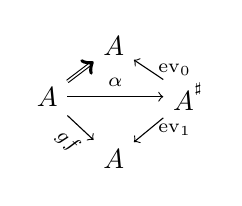
\begin{tikzpicture}[x=1.6em,y=1.4em]
  \node (At) at (1.5,2.4) {$A$};
  \node (Al) at (0,1.1) {$A$};
  \node (M) at (3.2,1.1) {$A^{\qcInt^{\sharp}}$};
  \node (Ab) at (1.5,-0.5) {$A$};
  \draw[double,->] (Al) -- (At);
  \draw[->] (Al) -- node[above]{$\scriptstyle\alpha$} (M);
  \draw[->] (M) -- node[right]{$\scriptstyle\mathrm{ev}_{0}$} (At);
  \draw[->] (M) -- node[right]{$\scriptstyle\mathrm{ev}_{1}$} (Ab);
  \draw[->] (Al) -- node[below,sloped]{$\scriptstyle gf$} (Ab);
\end{tikzpicture}
\qquad 与 \qquad
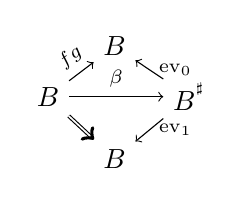
\begin{tikzpicture}[x=1.6em,y=1.4em]
  \node (Bt) at (1.5,2.4) {$B$};
  \node (Bl) at (0,1.1) {$B$};
  \node (M) at (3.2,1.1) {$B^{\qcInt^{\sharp}}$};
  \node (Bb) at (1.5,-0.5) {$B$};
  \draw[->] (Bl) -- node[above,sloped]{$\scriptstyle fg$} (Bt);
  \draw[->] (Bl) -- node[above]{$\scriptstyle\beta$} (M);
  \draw[->] (M) -- node[right]{$\scriptstyle\mathrm{ev}_{0}$} (Bt);
  \draw[->] (M) -- node[right]{$\scriptstyle\mathrm{ev}_{1}$} (Bb);
  \draw[double,->] (Bl) -- (Bb);
\end{tikzpicture}
\end{center}
反之，这样一份数据经限制便展现出一个复状单纯集的\trEquivalence。
\end{corollary}

\begin{proof}
\cref{def:complicial-equivalences}的数据可以提升如下：
\begin{center}
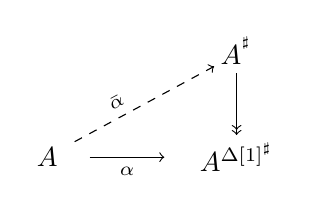
\begin{tikzpicture}[x=1.8em,y=1.6em]
  \node (m) at (3.8,1.2) {$A^{\qcInt^{\sharp}}$};
  \node (bl) at (0,-1.2) {$A$};
  \node (br) at (3.8,-1.2) {$A^{\Delta[1]^{\sharp}}$};
  \draw[->,dashed] (0.55,-0.85) -- node[above,sloped,pos=0.35]{$\scriptstyle\bar{\alpha}$} (3.35,0.85);
  \draw[->>] (3.8,0.7) -- (3.8,-0.7);
  \draw[->] (0.85,-1.2) -- node[below]{$\scriptstyle\alpha$} (2.35,-1.2);
\end{tikzpicture}
\qquad
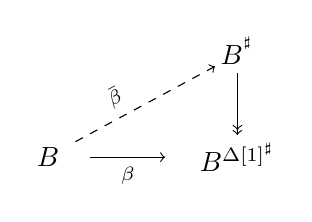
\begin{tikzpicture}[x=1.8em,y=1.6em]
  \node (m) at (3.8,1.2) {$B^{\qcInt^{\sharp}}$};
  \node (bl) at (0,-1.2) {$B$};
  \node (br) at (3.8,-1.2) {$B^{\Delta[1]^{\sharp}}$};
  \draw[->,dashed] (0.55,-0.85) -- node[above,sloped,pos=0.35]{$\scriptstyle\bar{\beta}$} (3.35,0.85);
  \draw[->>] (3.8,0.7) -- (3.8,-0.7);
  \draw[->] (0.85,-1.2) -- node[below]{$\scriptstyle\beta$} (2.35,-1.2);
\end{tikzpicture}
\end{center}
\end{proof}

我们想对\trQuasiCategory{}之间的\trIsofibration{}证明与
\cref{cor:leibniz-exponential}(iii) 与 (iv) 类比的命题，这需要与
\cref{prop:leibniz-marked-anodyne}及\cref{cor:leibniz-anodyne}类比的命题，
用以分析\trSimplicialSet{}的诸\trMonomorphism{}与包含
$\qcOne\hookrightarrow\qcInt$ 的\trLeibnizProduct。我们将通过考察%
\trQuasiCategory{}中的\trIsomorphism{}与复状单纯集中带标记边之间的关系
来推导这一点——这正是下一节的主题。

\subsection*{练习}

\begin{exercise}\label{ex:unmarked-leibniz-corollary}
陈述并证明\cref{cor:leibniz-mono-tf}的非带标记类比。
\end{exercise}

\begin{exercise}\label{ex:regular-entire-leibniz-products}
一个正则包含与一个非可逆的\trEntireInclusion{}的\trLeibnizProduct{}是\trEntireInclusion，但未必是正则包含。
找出展现这两种可能性的例子，并对那些必然正则的此类\trLeibnizProduct{}陈述并证明
一个刻画。这原本会简化\cref{prop:leibniz-marked-anodyne}的证明吗？
\end{exercise}

\begin{exercise}\label{ex:restriction-map-equivalence}
若 $f\colon X\to Y$ 是一个带标记\trHomotopyEquivalence{}而 $A$ 是一个复状
单纯集，证明：限制映射 $f^{*}\colon A^{Y}\to A^{X}$ 是复状单纯集间的一个%
\trEquivalence。
\end{exercise}

   %

\section{自然标记拟范畴中的同构}\label{sec:isomorphisms-naturally-marked-quasi-categories}

由\cref{ex:maximally-marked-kan}，\trKanComplex{}可以视为复状单纯集的一个
特例：也就是说，\trKanComplex{}恰与那些极大标记的复状单纯集相重合。在本节中，
我们将发现\trQuasiCategory{}同样可以与某些 1-平凡的复状单纯集（见\cref{def:n-trivial}）
相认同，其中带标记的 1-\trSimplex{}由底\trSimplicialSet{}所确定。在\cref{thm:natural-marking-complicial}中，
我们证明\trQuasiCategory{}的\trCategory{}可以与那些带标记 1-\trSimplex{}在某种
即将引入的精确意义下\emph{饱和}的 1-平凡复状单纯集相认同。

复状单纯集中 1-\trSimplex{}上的诸标记不能随意指派：每一条带标记的边都必须是
我们现在引入的意义下的一个\trEquivalence。

\begin{definition}[\trEquivalence]\label{def:equivalence-marked-simplicial-set}
带标记\trSimplicialSet{}中的一个 1-\trSimplex{} $f$ 是一个\textbf{\trEquivalence}，
若存在如下图所示的一对薄 2-\trSimplex：
\begin{center}
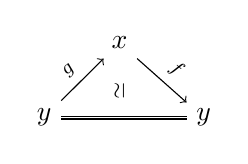
\begin{tikzpicture}[x=1.6em,y=1.35em]
  \node (x) at (1.7,2.0) {$x$};
  \node (yl) at (0,0) {$y$};
  \node (yr) at (3.6,0) {$y$};
  \draw[->] (yl) -- node[above,sloped,pos=0.45]{$\scriptstyle g$} (x);
  \draw[->] (x) -- node[above,sloped,pos=0.55]{$\scriptstyle f$} (yr);
  \draw[double] (yl) -- (yr);
  \node[rotate=90] at (1.7,0.72) {$\scriptstyle\simeq$};
\end{tikzpicture}
\qquad
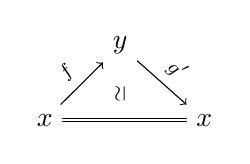
\begin{tikzpicture}[x=1.6em,y=1.35em]
  \node (y) at (1.7,2.0) {$y$};
  \node (xl) at (0,0) {$x$};
  \node (xr) at (3.6,0) {$x$};
  \draw[->] (xl) -- node[above,sloped,pos=0.45]{$\scriptstyle f$} (y);
  \draw[->] (y) -- node[above,sloped,pos=0.55]{$\scriptstyle g'$} (xr);
  \draw[double] (xl) -- (xr);
  \node[rotate=90] at (1.7,0.72) {$\scriptstyle\simeq$};
\end{tikzpicture}
\end{center}
\end{definition}

注意，\trEquivalence{}这一概念是相对于 2-\trSimplex{}上标记方式的选取而定义的。
对于\trQuasiCategory{}的边，一个非常相近的概念已在第 1 章中的\cref{def:isomorphism-quasi-category}
以「\trIsomorphism」之名得到定义。

\begin{lemma}\label{lem:marked-edges-equivalences}
复状单纯集中的每一条带标记的边都是一个\trEquivalence。
\end{lemma}

\begin{proof}
若 $f$ 是任一复状单纯集 $A$ 中的一条带标记的边，则第 0 面为 $f$ 而第 1 面
退化的那个 $\Lambda^{2}[2]$-\trHorn{}是容许的，故 $f$ 有一个右\trEquivalence{}逆。
一个涉及 $\Lambda^{0}[2]$-\trHorn{}的对偶构造表明 $f$ 还有一个左\trEquivalence{}逆：%
\footnote{又请注意，诸复状薄性扩张进一步蕴含这些单侧逆同样被标记，从而它们
容有各自的进一步的逆。}
\begin{center}
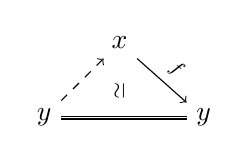
\begin{tikzpicture}[x=1.6em,y=1.35em]
  \node (x) at (1.7,2.0) {$x$};
  \node (yl) at (0,0) {$y$};
  \node (yr) at (3.6,0) {$y$};
  \draw[->,dashed] (yl) -- (x);
  \draw[->] (x) -- node[above,sloped,pos=0.55]{$\scriptstyle f$} (yr);
  \draw[double] (yl) -- (yr);
  \node[rotate=90] at (1.7,0.72) {$\scriptstyle\simeq$};
\end{tikzpicture}
\qquad
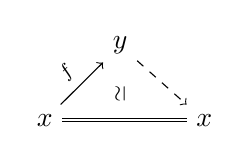
\begin{tikzpicture}[x=1.6em,y=1.35em]
  \node (y) at (1.7,2.0) {$y$};
  \node (xl) at (0,0) {$x$};
  \node (xr) at (3.6,0) {$x$};
  \draw[->] (xl) -- node[above,sloped,pos=0.45]{$\scriptstyle f$} (y);
  \draw[->,dashed] (y) -- (xr);
  \draw[double] (xl) -- (xr);
  \node[rotate=90] at (1.7,0.72) {$\scriptstyle\simeq$};
\end{tikzpicture}
\end{center}
\end{proof}

这一观察提示了给 1-\trCategory{}的\trNerve{}的边作标记的两种方式。

\begin{lemma}\label{lem:nerve-1-category-complicial}
一个 1-\trCategory{}的\trNerve{}定义一个复状单纯集，此时标记维数大于一的全部%
\trSimplex，然后以下列两种方式之一定义带标记的边：
\begin{enumerate}[label=(\roman*)]
\item 带标记的边仅为诸恒同箭头；或者
\item 带标记的边为全部\trIsomorphism。
\end{enumerate}
\end{lemma}

\begin{proof}
见\cref{ex:prove-lem-nerve-1-category}。
\end{proof}

这两种选取中的前者定义了使 1-\trCategory{}的\trNerve{}成为复状单纯集的极小
1-平凡标记。据\cref{lem:marked-edges-equivalences}，后者定义了使 1-\trCategory{}%
的\trNerve{}成为复状单纯集的极大标记。我们现在引入一套术语来描述「极大标记的」
1-平凡复状单纯集。

\begin{definition}[1-饱和的]\label{def:1-saturated}
一个复状单纯集是 \textbf{1-饱和的}（1-saturated），若它的诸边之中所含的每一个%
\trEquivalence{}都被标记。\footnote{由于在诸 1-\trSimplex{}之中刻画\trEquivalence{}%
需要预先约定哪些 2-\trSimplex{}被标记，我们通常将\cref{def:1-saturated}应用于
1-平凡的复状单纯集；此时我们简称一个 1-饱和的 1-平凡复状单纯集为「饱和的」
（saturated）。这是\cref{dig:saturation-higher-simplices}中所讨论的饱和复状
单纯集这一一般概念的一个特例。}
\end{definition}

这促成了下述\trQuasiCategory{}之典范标记的定义——它在 \cite{bib78} 中称作
「自然标记」。也就是说，我们赋予每个\trQuasiCategory{}其唯一的 1-饱和 1-平凡
标记：

\begin{definition}[自然标记]\label{def:natural-marking}
对任何\trQuasiCategory{} $A$，其\textbf{自然标记}定义如下：
\begin{itemize}
\item 标记维数大于一的全部\trSimplex{}；
\item 恰好标记那些作为\trIsomorphism{}的边（第 1 章中的\cref{def:isomorphism-quasi-category}
  的意义下），或者等价地，标记全部那些作为\trEquivalence{}的边
  （\cref{def:equivalence-marked-simplicial-set} 的意义下）。
\end{itemize}
\end{definition}

\trQuasiCategory{}的自然标记便于陈述并证明一个归功于 Joyal 的重要组合结果：

\begin{proposition}\label{prop:outer-complicial-horn-fillings}
任何自然标记\trQuasiCategory{} $A$ 对 $n\ge 1$ 容有外复状号角扩张的\trFiller：
\begin{center}
\begin{tikzpicture}[x=1.6em,y=1.4em]
  \node (lt) at (0,1.2) {$\Lambda^{0}[n]$};
  \node (rt) at (2.8,1.2) {$A$};
  \node (lb) at (0,-1.2) {$\Delta^{0}[n]$};
  \draw[->] (lt) -- (rt);
  \draw[right hook->] (lb) -- (lt);
  \node at (-0.45,0) {$\scriptstyle r$};
  \draw[->,dashed] (0.45,-1.0) -- (2.35,1.0);
\end{tikzpicture}
\qquad
\begin{tikzpicture}[x=1.6em,y=1.4em]
  \node (lt) at (0,1.2) {$\Lambda^{n}[n]$};
  \node (rt) at (2.8,1.2) {$A$};
  \node (lb) at (0,-1.2) {$\Delta^{n}[n]$};
  \draw[->] (lt) -- (rt);
  \draw[right hook->] (lb) -- (lt);
  \node at (-0.45,0) {$\scriptstyle r$};
  \draw[->,dashed] (0.45,-1.0) -- (2.35,1.0);
\end{tikzpicture}
\end{center}
\end{proposition}

在原始文献 \cite{bib61} 中，该结果不带标记地陈述如下：一个\trQuasiCategory{}%
对\textbf{特殊外\trHorn}容有\trFiller——即初始 $\{01\}$-边被映成 $A$ 中一个%
\trIsomorphism{}的左\trHorn{} $\Lambda^{0}[n]\to A$，以及末端 $\{n{-}1\,n\}$-边
被映成 $A$ 中一个\trIsomorphism{}的右\trHorn{} $\Lambda^{n}[n]\to A$。

\cref{prop:outer-complicial-horn-fillings}的诸多证明都是可能的；例如见
\cite[\S B]{bib36} 或原始文献 \cite{bib61}。我们选择采用 \trVerity{}的组合结果
\cite[\S4.2]{bib129}，并分期予以陈述；这些结果使用了\trHomotopyCoherentIsomorphism
的一个替代概念（事后可见与之等价）——同伦类型论家会凭「半伴随等价」
（half adjoint equivalence）之名认出它 \cite[\S4.2]{bib125}。

\begin{notation}[相干同构的子复形]\label{not:subcomplexes-coherent-isomorphism}
回顾\textbf{相干同构}（coherent isomorphism）：即定义为\trFreeLivingIsomorphism
之\trNerve{}的那个\trSimplicialSet{} $\qcInt$。它在每一维恰有两个非退化%
\trSimplex。若把它的顶点标作「$-$」与「$+$」，则其余非退化\trSimplex{}便由其
顶点唯一确定，这些顶点即从任一端出发的「$-$」与「$+$」的交错序列。作为%
\trMarkedSimplicialSet，我们赋予 $\qcInt$ 及其子复形（subcomplexes）极大标记。
\end{notation}

沿 \cite{bib129,bib42} 引入的记号，我们记 $E_{n}^{\pm}$、$E_{n}^{\mp}\subset\qcInt$
为分别由 $n$-\trSimplex{} $-+-\cdots\pm$ 与 $+-+\cdots\mp$ 生成的单纯子集。两个
单纯子集均唯一地嵌入 $E_{n+1}^{\mp}$ 与 $E_{n+1}^{\pm}$ 两者，且这些包含按如下
方式分解
\begin{center}
\begin{tikzpicture}[x=1.05em,y=1.3em]
  \node (lt1) at (0,3.2) {$\Lambda^{0}[n+1]$};
  \node (rt1) at (5.4,3.2) {$E_{n}^{\pm}$};
  \node (lb1) at (0,1.0) {$\Delta^{0}[n+1]$};
  \node (bul1) at (5.4,1.0) {$\bullet$};
  \node (rb1) at (10.8,1.0) {$\Delta^{0}[n+1]'$};
  \node (bb1) at (5.4,-1.4) {$E_{n+1}^{\pm}$};
  \node (rb2) at (10.8,-1.4) {$\Delta^{0}[n+1]''$};
  \draw[->] (lt1) -- (rt1);
  \draw[right hook->] (lb1) -- node[pos=0.5,left]{$\scriptstyle r$} (lt1);
  \draw[right hook->] (rt1) -- (bul1);
  \draw[->] (lb1) -- (bul1);
  \node at (4.75,1.28) {$\scriptstyle\llcorner$};
  \draw[->] (rb1) -- (bul1);
  \draw[->] (bul1) -- (bb1);
  \node at (4.75,-0.95) {$\scriptstyle\llcorner$};
  \draw[right hook->] (rb2) -- node[pos=0.5,right]{$\scriptstyle e$} (rb1);
  \draw[->] (rb2) -- (bb1);
  \node (lt2) at (14.0,3.2) {$\Lambda^{n+1}[n+1]$};
  \node (rt2) at (20.6,3.2) {$E_{n}^{\pm}$};
  \node (lb2) at (14.0,1.0) {$\Delta^{n+1}[n+1]$};
  \node (bul2) at (20.6,1.0) {$\bullet$};
  \node (rb3) at (27.2,1.0) {$\Delta^{n+1}[n+1]'$};
  \node (bb2) at (20.6,-1.4) {$E_{n+1}^{\pm}$};
  \node (rb4) at (27.2,-1.4) {$\Delta^{n+1}[n+1]''$};
  \draw[->] (lt2) -- (rt2);
  \draw[right hook->] (lb2) -- node[pos=0.5,left]{$\scriptstyle r$} (lt2);
  \draw[right hook->] (rt2) -- (bul2);
  \draw[->] (lb2) -- (bul2);
  \node at (19.95,1.28) {$\scriptstyle\llcorner$};
  \draw[->] (rb3) -- (bul2);
  \draw[->] (bul2) -- (bb2);
  \node at (19.95,-0.95) {$\scriptstyle\llcorner$};
  \draw[right hook->] (rb4) -- node[pos=0.5,right]{$\scriptstyle e$} (rb3);
  \draw[->] (rb4) -- (bb2);
\end{tikzpicture}
\end{center}
从而证明了任何满足 $m>n$ 的包含 $E_{n}^{\pm}\hookrightarrow E_{m}^{\pm}$ 或
$E_{n}^{\mp}\hookrightarrow E_{m}^{\pm}$ 都是带标记\trAnodyneExtension。

下述结果给出一个判据，用以断定一个\textbf{内复状纤维化}（inner complicial
fibration）——即只假定了对诸内复状号角扩张与诸内复状薄性扩张具有右提升性质的
带标记映射——何时在事实上定义一个复状等价纤维化。

\begin{proposition}\label{prop:inner-complicial-fibration-criterion}
设 $p\colon A\twoheadrightarrow B$ 是一个内复状纤维化，其余定义域 $B$ 是一个
复状单纯集。则 $p$ 是一个复状等价纤维化，当且仅当 $p$ 对包含
$E_{0}^{-}\hookrightarrow E_{1}^{-}$ 与 $E_{1}^{-}\hookrightarrow E_{3}^{-}$
容有提升。
\end{proposition}

\begin{proof}
任何复状等价纤维化都对带标记\trAnodyneExtension $E_{0}^{-}\hookrightarrow E_{1}^{-}$ 与
$E_{1}^{-}\hookrightarrow E_{3}^{-}$ 容有提升。于是，本结果的核心，也是唯一
尚待证明的部分，即是如下断言：任何对这一对包含容有提升、且余定义域为复状
单纯集的内复状纤维化，必然也对外复状号角扩张与外复状薄性扩张容有\trFiller。

我们先论证：满足陈述条件的内复状纤维化 $p\colon A\twoheadrightarrow B$ 也对
对偶包含 $E_{0}^{-}\hookrightarrow E_{1}^{+}$ 容有提升。给定如下方块中由映射
$a$ 与 $b$ 呈现的提升问题：
\begin{center}
\begin{tikzpicture}[x=1.6em,y=1.4em]
  \node (e0) at (0.6,2.4) {$E_{0}^{-}$};
  \node (A)  at (4.4,2.4) {$A$};
  \node (e1m) at (-2.4,0.7) {$E_{1}^{-}$};
  \node (e1p) at (0.6,0.7) {$E_{1}^{+}$};
  \node (B)  at (4.4,0.7) {$B$};
  \node (e3) at (0.6,-1.5) {$E_{3}^{-}$};
  \draw[->] (e1m) -- (e0);
  \draw[->] (e1m) -- (e3);
  \draw[right hook->] (e0) -- (e1p);
  \draw[right hook->] (e1p) -- (e3);
  \draw[->] (e0) -- node[above]{$\scriptstyle a$} (A);
  \draw[->] (e1p) -- node[above]{$\scriptstyle b$} (B);
  \draw[->] (A) -- node[right]{$\scriptstyle p$} (B);
  \draw[->,dashed] (e3) -- (B);
  \draw[->,dotted] (e1p) -- (A);
\end{tikzpicture}
\end{center}
则存在 $b$ 沿 $E_{1}^{+}\hookrightarrow E_{3}^{-}$ 的虚线\trExtension，因为该
包含是带标记\trAnodyneExtension{}且 $B$ 是复状单纯集。现在，包含 $E_{0}^{-}\hookrightarrow E_{3}^{-}$
如所示分解为 $E_{0}^{-}\hookrightarrow E_{1}^{+}\hookrightarrow E_{3}^{-}$，而
由假设 $p$ 对这两个映射均可提升，故点线提升也存在，它经限制便定义了原提升问题
的一个解。

手持这一结果，立即可知 $p\colon A\twoheadrightarrow B$ 的奇对偶满足与
$p\colon A\twoheadrightarrow B$ 相同的提升性质，因为 $E_{0}^{-}\hookrightarrow E_{1}^{-}$
的奇对偶是 $E_{0}^{-}\hookrightarrow E_{1}^{+}$，而 $E_{1}^{-}\hookrightarrow E_{3}^{-}$
的奇对偶同构于其自身。于是只须证明：$p$ 对左复状号角扩张
$\Lambda^{0}[n]\hookrightarrow_{r}\Delta^{0}[n]$ 与左复状薄性扩张
$\Delta^{0}[n]'\hookrightarrow_{e}\Delta^{0}[n]''$ 容有提升即可，此时其奇对偶
将分享这些性质，这蕴含 $p$ 对右复状号角扩张与右复状薄性扩张也容有提升。情形
$\Lambda^{0}[1]\hookrightarrow\Delta^{0}[1]$ 即映射 $E_{0}^{-}\hookrightarrow E_{1}^{-}$，
故还可设 $n>1$，此时我们有同构
\[
\Lambda^{0}[n]\hookrightarrow\Delta^{0}[n]
\cong(\Lambda^{0}[1]\hookrightarrow\Delta^{0}[1])\mathbin{\hat{\star}}
(\partial\Delta[n-2]\hookrightarrow\Delta[n-2])\text{，}
\]
由\cref{lem:leibniz-join-complicial}。为简便计记 $m=n-2$，考虑由映射 $a$ 与
$b$ 呈现的提升问题：
\begin{center}
\begin{tikzpicture}[x=1.0em,y=1.4em]
  \node (tl) at (0,1.7) {$E_{0}^{-}\star\Delta[m]\cup E_{1}^{-}\star\partial\Delta[m]$};
  \node (tr) at (14.6,1.7) {$A$};
  \node (bl) at (0,-0.7) {$E_{1}^{-}\star\Delta[m]$};
  \node (bm) at (7.3,-0.7) {$E_{2}^{-}\star\Delta[m]_{t}\cup E_{3}^{-}\star\partial\Delta[m]$};
  \node (br) at (14.6,-0.7) {$E_{3}^{-}\star\Delta[m]$};
  \node (B) at (17.2,-0.7) {$B$};
  \draw[->] (tl) -- node[above]{$\scriptstyle a$} (tr);
  \draw[right hook->] (tl) -- node[pos=0.45,left]{$\scriptstyle i$} (bl);
  \draw[right hook->] (bl) -- (bm);
  \draw[right hook->] (bm) -- (br);
  \draw[->,dashed] (br) -- (B);
  \draw[->] (tr) -- node[right]{$\scriptstyle p$} (B);
  \draw[->,dotted] (bm) -- (tr);
  \draw[->] (bl) to[bend right=12] node[below,pos=0.55]{$\scriptstyle j$} (br);
  \draw[->] (bl) to[bend right=20] node[below,pos=0.55]{$\scriptstyle b$} (B);
\end{tikzpicture}
\end{center}
据\cref{lem:leibniz-join-complicial}，映射 $j$ 是带标记\trAnodyneExtension，故由于 $B$ 是
复状单纯集，虚线\trExtension{}存在。为证明点线提升也存在，我们论证：映射 $i$
由诸内复状号角扩张与映射 $E_{1}^{-}\hookrightarrow E_{3}^{-}$ 胞腔式生成。为
看到这一点，将映射 $i$ 分解为

\begin{rveq}\label{eq:pushout-squares-factorization}
\begin{tikzpicture}[x=1.0em,y=1.35em]
  \node (a) at (0,3.4) {$E_{1}^{-}$};
  \node (b) at (7.0,3.4) {$E_{0}^{-}\star\Delta[m]\cup E_{1}^{-}\star\partial\Delta[m]$};
  \node (c) at (0,1.7) {$E_{3}^{-}$};
  \node (d) at (7.0,1.7) {$\bullet$};
  \node (e) at (14.6,1.7) {$E_{1}^{-}\star\partial\Delta[m]\cup E_{3}^{-}\star\varnothing$};
  \node (f) at (0,0) {$E_{0}^{-}\star\Delta[m]\cup E_{2}^{-}\star\partial\Delta[m]$};
  \node (g) at (7.0,0) {$\bullet$};
  \node (h) at (14.6,0) {$E_{3}^{-}\star\partial\Delta[m]$};
  \node (i) at (0,-1.7) {$E_{2}^{-}\star\Delta[m]$};
  \node (j) at (7.0,-1.7) {$E_{2}^{-}\star\Delta[m]\cup E_{3}^{-}\star\partial\Delta[m]$};
  \draw[right hook->] (a) -- (b);
  \draw[right hook->] (a) -- (c);
  \draw[right hook->] (b) -- (d);
  \draw[->] (c) -- (d);
  \node at (6.35,1.95) {$\scriptstyle\llcorner$};
  \draw[right hook->] (e) -- (d);
  \draw[->] (d) -- (g);
  \draw[right hook->] (e) -- (h);
  \draw[->] (h) -- (g);
  \node at (6.35,0.25) {$\scriptstyle\llcorner$};
  \draw[right hook->] (f) -- (g);
  \draw[right hook->] (f) -- (i);
  \draw[->] (g) -- (j);
  \draw[right hook->] (i) -- (j);
  \node at (6.35,-1.4) {$\scriptstyle\llcorner$};
\end{tikzpicture}
\end{rveq}

第一个附贴胞腔就是映射 $E_{1}^{-}\hookrightarrow E_{3}^{-}$ 本身。如
\cref{not:subcomplexes-coherent-isomorphism} 中所观察，$E_{1}^{-}\hookrightarrow E_{3}^{-}$
是一个右\trAnodyneExtension，故据\cref{lem:leibniz-join-complicial}，第二个附贴胞腔
$(E_{1}^{-}\hookrightarrow E_{3}^{-})\mathbin{\hat{\star}}(\varnothing\hookrightarrow\partial\Delta[m])$
是一个内\trAnodyneExtension。类似地 $E_{0}^{-}\hookrightarrow E_{2}^{-}$ 是一个右\trAnodyneExtension，
故最后一个附贴胞腔
$(E_{0}^{-}\hookrightarrow E_{2}^{-})\mathbin{\hat{\star}}(\partial\Delta[m]\hookrightarrow\Delta[m])$
也是一个内\trAnodyneExtension。从而，$p$ 对诸左复状号角扩张容有提升，如所断言。

为看出 $p\colon A\to B$ 也对外复状薄性扩张容有提升，我们利用\cref{lem:leibniz-join-complicial}
的下述同构
\[
(\Lambda^{0}[1]\hookrightarrow\Delta^{0}[1])\mathbin{\hat{\star}}(\Delta[m]\hookrightarrow\Delta[m]_{t})
\cong
\Delta^{0}[m+2]'\hookrightarrow\Delta^{0}[m+2]''\text{，}
\]
忆及 $\Lambda^{0}[1]\hookrightarrow\Delta^{0}[1]$ 即包含 $E_{0}^{-}\hookrightarrow E_{1}^{-}$。
于是我们可以考虑由映射 $a$ 与 $b$ 呈现的提升问题：
\begin{center}
\begin{tikzpicture}[x=1.0em,y=1.4em]
  \node (tl) at (0,1.7) {$E_{0}^{-}\star\Delta[m]_{t}\cup E_{1}^{-}\star\Delta[m]$};
  \node (tr) at (14.6,1.7) {$A$};
  \node (bl) at (0,-0.7) {$E_{1}^{-}\star\Delta[m]_{t}$};
  \node (bm) at (7.3,-0.7) {$E_{2}^{-}\star\Delta[m]\cup E_{3}^{-}\star\Delta[m]$};
  \node (br) at (14.6,-0.7) {$E_{3}^{-}\star\Delta[m]_{t}$};
  \node (B) at (17.2,-0.7) {$B$};
  \draw[->] (tl) -- node[above]{$\scriptstyle a$} (tr);
  \draw[right hook->] (tl) -- node[pos=0.45,left]{$\scriptstyle i$} (bl);
  \draw[right hook->] (bl) -- (bm);
  \draw[right hook->] (bm) -- (br);
  \draw[->,dashed] (br) -- (B);
  \draw[->] (tr) -- node[right]{$\scriptstyle p$} (B);
  \draw[->,dotted] (bm) -- (tr);
  \draw[->] (bl) to[bend right=12] node[below,pos=0.55]{$\scriptstyle j$} (br);
  \draw[->] (bl) to[bend right=20] node[below,pos=0.55]{$\scriptstyle b$} (B);
\end{tikzpicture}
\end{center}
据\cref{lem:leibniz-join-complicial}，映射 $j$ 是带标记\trAnodyneExtension，故由于 $B$ 是
复状单纯集，虚线\trExtension{}存在。为证明点线提升也存在，我们论证：映射 $i$
由诸内复状号角扩张、诸内复状薄性扩张与映射 $E_{1}^{-}\hookrightarrow E_{3}^{-}$
胞腔式生成。为看到这一点，将映射 $i$ 分解为

\begin{center}
\begin{tikzpicture}[x=1.0em,y=1.35em]
  \node (a) at (0,3.4) {$E_{1}^{-}$};
  \node (b) at (7.0,3.4) {$E_{0}^{-}\star\Delta[m]_{t}\cup E_{1}^{-}\star\Delta[m]$};
  \node (c) at (0,1.7) {$E_{3}^{-}$};
  \node (d) at (7.0,1.7) {$\bullet$};
  \node (e) at (14.6,1.7) {$E_{1}^{-}\star\Delta[m]\cup E_{3}^{-}\star\varnothing$};
  \node (f) at (0,0) {$E_{0}^{-}\star\Delta[m]_{t}\cup E_{2}^{-}\star\Delta[m]$};
  \node (g) at (7.0,0) {$\bullet$};
  \node (h) at (14.6,0) {$E_{3}^{-}\star\Delta[m]$};
  \node (i) at (0,-1.7) {$E_{2}^{-}\star\Delta[m]_{t}$};
  \node (j) at (7.0,-1.7) {$E_{2}^{-}\star\Delta[m]_{t}\cup E_{3}^{-}\star\Delta[m]$};
  \draw[right hook->] (a) -- (b);
  \draw[right hook->] (a) -- (c);
  \draw[right hook->] (b) -- (d);
  \draw[->] (c) -- (d);
  \node at (6.35,1.95) {$\scriptstyle\llcorner$};
  \draw[right hook->] (e) -- (d);
  \draw[->] (d) -- (g);
  \draw[right hook->] (e) -- (h);
  \draw[->] (h) -- (g);
  \node at (6.35,0.25) {$\scriptstyle\llcorner$};
  \draw[right hook->] (f) -- (g);
  \draw[right hook->] (f) -- (i);
  \draw[->] (g) -- (j);
  \draw[right hook->] (i) -- (j);
  \node at (6.35,-1.4) {$\scriptstyle\llcorner$};
\end{tikzpicture}
\end{center}

第一个附贴胞腔就是映射 $E_{1}^{-}\hookrightarrow E_{3}^{-}$ 本身。如
\cref{not:subcomplexes-coherent-isomorphism} 中所观察，$E_{1}^{-}\hookrightarrow E_{3}^{-}$
是一个右带标记\trAnodyneExtension，故据\cref{lem:leibniz-join-complicial}，第二个附贴胞腔
$(E_{1}^{-}\hookrightarrow E_{3}^{-})\mathbin{\hat{\star}}(\varnothing\hookrightarrow\Delta[m])$
是一个内带标记\trAnodyneExtension。类似地 $E_{0}^{-}\hookrightarrow E_{2}^{-}$ 是一个右%
\trAnodyneExtension，故最后一个附贴胞腔
$(E_{0}^{-}\hookrightarrow E_{2}^{-})\mathbin{\hat{\star}}(\Delta[m]\hookrightarrow\Delta[m]_{t})$
也是一个内复状薄性扩张。从而，$p$ 对诸左复状薄性扩张容有提升，如所断言。
\end{proof}

由于包含 $E_{0}^{-}\hookrightarrow E_{1}^{-}$ 与 $E_{1}^{-}\hookrightarrow E_{3}^{-}$
是左带标记\trAnodyneExtension，\cref{prop:inner-complicial-fibration-criterion} 立得下述
推论。

\begin{corollary}\label{cor:left-right-complicial-fibration}
设 $p\colon A\twoheadrightarrow B$ 是一个内复状纤维化，其余定义域 $B$ 是一个
复状单纯集。则当 $p$ 是一个左复状纤维化或一个右复状纤维化时，$p$ 是一个复状
等价纤维化。
\end{corollary}

请注意，在\cref{prop:inner-complicial-fibration-criterion}的证明中，对包含
$E_{0}^{-}\hookrightarrow E_{1}^{-}$ 的提升只是在构造外复状号角扩张
$\Lambda^{0}[1]\hookrightarrow\Delta^{0}[1]$ 与 $\Lambda^{1}[1]\hookrightarrow\Delta^{1}[1]$
的提升时才需要。于是，即便去掉这一提升条件，更高维数的外复状号角扩张仍可
构造出来。刚才给出的论证给出了「特殊外\trHorn{}填充」的一个特例的证明，这一
特例在证明一般版本时有用。

\begin{lemma}\label{lem:left-horn-filling-degenerate-edge}
设 $p\colon A\twoheadrightarrow B$ 是一个内复状纤维化，其余定义域 $B$ 是一个
复状单纯集。则 $p$ 对左\trHorn
\begin{center}
\begin{tikzpicture}[x=1.6em,y=1.4em]
  \node (lt) at (0,1.2) {$\Lambda^{0}[n]$};
  \node (rt) at (2.8,1.2) {$A$};
  \node (lb) at (0,-1.2) {$\Delta^{0}[n]$};
  \node (rb) at (2.8,-1.2) {$B$};
  \draw[->] (lt) -- node[above]{$\scriptstyle a$} (rt);
  \draw[right hook->] (lb) -- (lt);
  \draw[->] (lb) -- node[below]{$\scriptstyle b$} (rb);
  \draw[->] (rt) -- node[right]{$\scriptstyle p$} (rb);
  \draw[->,dashed] (0.45,-1.0) -- (2.35,1.0);
\end{tikzpicture}
\end{center}
（$n>1$）容有\trFiller，只要 $a$ 把\trHorn{} $\Lambda^{0}[n]$ 的 $\{01\}$ 边
送到 $A$ 中一个退化\trSimplex。
\end{lemma}

\begin{proof}
记 $m=n-2$。据\cref{lem:leibniz-join-complicial}，我们有同构
\[
\Lambda^{0}[m+2]\hookrightarrow\Delta^{0}[m+2]
\cong(\Lambda^{0}[1]\hookrightarrow\Delta^{0}[1])\mathbin{\hat{\star}}
(\partial\Delta[m]\hookrightarrow\Delta[m])\text{，}
\]
于是我们再一次被要求考虑由映射 $a$ 与 $b$ 呈现的提升问题：
\begin{center}
\begin{tikzpicture}[x=1.0em,y=1.4em]
  \node (tl) at (0,1.9) {$E_{0}^{-}\star\Delta[m]\cup E_{1}^{-}\star\partial\Delta[m]$};
  \node (tm) at (8.2,1.9) {$E_{0}^{-}\star\Delta[m]\cup E_{1}^{-}\star\partial\Delta[m]\underset{E_{1}^{-}}{\cup}E_{3}^{-}$};
  \node (tr) at (17.4,1.9) {$A$};
  \node (bl) at (0,-0.9) {$E_{1}^{-}\star\Delta[m]$};
  \node (bm) at (8.2,-0.9) {$E_{2}^{-}\star\Delta[m]\cup E_{3}^{-}\star\partial\Delta[m]$};
  \node (br) at (17.4,-0.9) {$E_{3}^{-}\star\Delta[m]$};
  \node (B) at (20.0,-0.9) {$B$};
  \draw[->] (tl) to[bend left=18] node[above,pos=0.4]{$\scriptstyle a$} (tr);
  \draw[right hook->] (tl) -- node[below,pos=0.5]{$\scriptstyle k$} (tm);
  \draw[->,dashed] (tm) -- (tr);
  \draw[right hook->] (tl) -- node[pos=0.45,left]{$\scriptstyle i$} (bl);
  \draw[right hook->] (tm) -- node[pos=0.45,right]{$\scriptstyle\ell$} (bm);
  \draw[right hook->] (bl) -- (bm);
  \draw[right hook->] (bm) -- (br);
  \draw[->,dashed] (br) -- (B);
  \draw[->] (tr) -- node[right]{$\scriptstyle p$} (B);
  \draw[->,dotted] (bm) -- (tr);
  \draw[->] (bl) to[bend right=12] node[below,pos=0.55]{$\scriptstyle j$} (br);
  \draw[->] (bl) to[bend right=20] node[below,pos=0.55]{$\scriptstyle b$} (B);
\end{tikzpicture}
\end{center}
映射 $j$ 是带标记\trAnodyneExtension，故由于 $B$ 是复状单纯集，下方的虚线\trExtension{}%
存在，于是只剩下求解映射 $i$ 与映射 $p$ 之间的提升问题。为此，我们把映射 $i$
分解为 \eqref{eq:pushout-squares-factorization} 中所示的中间一列三个竖直态射的
复合，并令 $k$ 记这些态射中的第一个，而 $\ell$ 记后两个的复合。接下来，通过
指定被附贴的 $E_{3}^{-}$ 的像为一个退化 3-\trSimplex{}来求解 $k$ 与 $p$ 之间
的提升问题；注意 $k$ 的构造方式是把该 $E_{3}^{-}$ 附贴到对应于号角
$\Lambda^{0}[m+2]$ 之初始边的那只 $E_{1}^{-}$ 上，而 $a$ 把这条边送到一条退化边。

现在，为构造点线提升，只剩下求解 $\ell$ 与 $p$ 之间的提升问题，而
\eqref{eq:pushout-squares-factorization} 揭示这可以做到：它把映射 $\ell$ 表为
诸内复状号角扩张的推出之复合。
\end{proof}

\begin{corollary}\label{cor:inner-fillings-complicial-set}
一个对诸内复状号角扩张与诸内复状薄性扩张容有\trFiller{}的带标记\trSimplicialSet
$A$ 是一个复状单纯集，当且仅当它沿 $\Delta[1]^{\sharp}\hookrightarrow\mathrm{sk}_{2}\qcInt^{\sharp}$
容有\trExtension。
\end{corollary}

\begin{proof}
把\cref{prop:inner-complicial-fibration-criterion}应用于内复状纤维化
$A\to\qcOne$：为断定 $A$ 是一个复状单纯集，只须沿映射 $E_{0}^{-}\hookrightarrow E_{1}^{-}$
与 $E_{1}^{-}\hookrightarrow E_{3}^{-}$ 构造\trExtension。前者是自动的，因为
$E_{0}^{-}\hookrightarrow E_{1}^{-}$ 同构于 $\Delta[0]\hookrightarrow\Delta[1]^{\sharp}$，
而后者容有一个收缩，所以为完成证明，我们将表明：在所述假设下，若 $A$ 沿映射
$E_{1}^{-}\hookrightarrow E_{3}^{-}$ 容有\trExtension，则结论成立。

定义域映射 $\Delta[1]^{\sharp}\cong E_{1}^{-}\to A$ 定义 $A$ 中一个带标记
1-\trSimplex{} $f\colon x\to y$，据假设我们可以把它\trExtension{}成映射
$\mathrm{sk}_{2}\qcInt^{\sharp}\to A$，后者指明诸带标记 2-\trSimplex
\begin{center}
\begin{tikzpicture}[x=1.6em,y=1.35em]
  \node (y) at (1.7,2.0) {$y$};
  \node (xl) at (0,0) {$x$};
  \node (xr) at (3.6,0) {$x$};
  \draw[->] (xl) -- node[above,sloped,pos=0.45]{$\scriptstyle f$} (y);
  \draw[->] (y) -- node[above,sloped,pos=0.55]{$\scriptstyle f^{-1}$} (xr);
  \draw[double] (xl) -- (xr);
  \node at (1.55,1.35) {$\scriptstyle\alpha$};
  \node[rotate=90] at (1.7,0.72) {$\scriptstyle\simeq$};
\end{tikzpicture}
\qquad
\begin{tikzpicture}[x=1.6em,y=1.35em]
  \node (x) at (1.7,2.0) {$x$};
  \node (yl) at (0,0) {$y$};
  \node (yr) at (3.6,0) {$y$};
  \draw[->] (yl) -- node[above,sloped,pos=0.45]{$\scriptstyle f^{-1}$} (x);
  \draw[->] (x) -- node[above,sloped,pos=0.55]{$\scriptstyle f$} (yr);
  \draw[double] (yl) -- (yr);
  \node at (1.55,1.35) {$\scriptstyle\alpha'$};
  \node[rotate=90] at (1.7,0.72) {$\scriptstyle\simeq$};
\end{tikzpicture}
\end{center}
2-\trSimplex{} $\alpha$ 与 $\alpha'$ 可以理解为定义二维\trEquivalence{}
$\alpha\colon\mathrm{id}_{x}\simeq f^{-1}f$ 与
$\alpha'\colon\mathrm{id}_{y}\simeq ff^{-1}$。$\alpha$ 与 $\alpha'$ 这一对
2-\trSimplex{}未必构成映射 $E_{3}^{-}\to A$ 的两个非退化 2-\trSimplex{}面——
那将等同于附加要求：三角恒等复合 $(\alpha')^{-1}f\cdot f\alpha$ \trEquivalence{}%
于 $\mathrm{id}_{f}$，\footnote{这正是为什么带标记\trSimplicialSet{} $E_{3}^{-}$
与 $E_{3}^{+}$ 或许可被称作「半伴随等价」的缘由。}但我们将构造 $\alpha'$ 的一个
替代 $\beta$，使得 $\alpha$ 与 $\beta$ 构成 $E_{3}^{-}\to A$ 的非退化
2-\trSimplex。\footnote{这应当与第 2 章中经由\cref{lem:minimal-adjunction-data}
的\cref{prop:adjoint-equivalences}之证明相对照。}

3-\trSimplex{} $E_{3}^{-}$ 将被构造为我们即将搭建的号角 $\Lambda^{2}[4]\to A$
之\trFiller{}的第 2 面。作为对下述构造的定向指引，我们先总结最终结果：
\begin{itemize}
\item 第 0、第 2 与第 3 个顶点将是 $x$，而第 1 与第 4 个顶点将是 $y$；
\item 全部边都将是 $\mathrm{id}_{x}$、$\mathrm{id}_{y}$、$f$ 或 $f^{-1}$，
  其位置由诸顶点唯一确定；
\item 面 $\{0,1,2\}$ 与 $\{0,1,3\}$ 是 $\alpha$，而面 $\{1,2,4\}$ 是 $\alpha'$；
\item 面 $\{0,2,3\}$、$\{0,1,4\}$、$\{0,3,4\}$ 与 $\{1,2,3\}$ 是退化的；而
\item 缺失的面 $\{0,2,4\}$（称作 $\gamma$）、$\{2,3,4\}$（称作 $\bar{\gamma}$）
  与 $\{1,3,4\}$（称作 $\beta$）将按此顺序填入，所需的 3-\trSimplex{} $E_{3}^{-}$
  即作为号角的第 2 面出现。
\end{itemize}

第 4 面是经退化而得的 3-\trSimplex{} $\alpha\sigma^{2}$。第 3 面通过填充如下图
所示的号角 $\Lambda^{1}[3]\to A$ 而构造：
\begin{center}
\mbox{\begin{tikzpicture}[x=1.7em,y=1.3em]
  \node (yt) at (1.1,2.2) {$y$};
  \node (xt) at (4.3,2.2) {$x$};
  \node (xb) at (0,0) {$x$};
  \node (yb) at (5.4,0) {$y$};
  \draw[->] (xb) -- node[above,sloped,pos=0.45]{$\scriptstyle f$} (yt);
  \draw[->] (yt) -- node[above]{$\scriptstyle f^{-1}$} (xt);
  \draw[->] (xt) -- node[above,sloped,pos=0.55]{$\scriptstyle f$} (yb);
  \draw[->] (xb) -- node[below]{$\scriptstyle f$} (yb);
  \node at (1.5,1.45) {$\scriptstyle\alpha$};
  \node[rotate=90] at (1.05,1.0) {$\scriptstyle\simeq$};
  \draw[double] (yt) .. controls (2.6,1.1) .. (yb);
  \node at (3.3,0.85) {$\scriptstyle\gamma$};
\end{tikzpicture}}
\quad$\simeq$\quad
\mbox{\begin{tikzpicture}[x=1.7em,y=1.3em]
  \node (yt) at (1.1,2.2) {$y$};
  \node (xt) at (4.3,2.2) {$x$};
  \node (xb) at (0,0) {$x$};
  \node (yb) at (5.4,0) {$y$};
  \draw[->] (xb) -- node[above,sloped,pos=0.45]{$\scriptstyle f$} (yt);
  \draw[->] (yt) -- node[above]{$\scriptstyle f^{-1}$} (xt);
  \draw[->] (xt) -- node[above,sloped,pos=0.55]{$\scriptstyle f$} (yb);
  \draw[->] (xb) -- node[below]{$\scriptstyle f$} (yb);
  \node at (3.6,1.5) {$\scriptstyle\alpha'$};
  \node[rotate=90] at (3.95,1.05) {$\scriptstyle\simeq$};
  \draw[double] (2.0,2.0) -- (2.0,0.4);
\end{tikzpicture}}
\end{center}
据一次复状薄性扩张，由填充该号角所定义的面 $\gamma$ 被标记。接着，第 1 面通过
填充号角 $\Lambda^{0}[3]\to A$ 构造，如\cref{lem:left-horn-filling-degenerate-edge}
所容许：

\begin{center}
\mbox{\begin{tikzpicture}[x=1.7em,y=1.3em]
  \node (xl) at (1.1,2.2) {$x$};
  \node (xr) at (4.3,2.2) {$x$};
  \node (xb) at (0,0) {$x$};
  \node (yb) at (5.4,0) {$y$};
  \draw[double] (xl) -- (xr);
  \draw[double] (xb) .. controls (0.6,1.4) .. (xl);
  \draw[->] (xr) -- node[above,sloped,pos=0.55]{$\scriptstyle f$} (yb);
  \draw[->] (xb) -- node[below]{$\scriptstyle f$} (yb);
  \draw[double] (2.1,1.9) -- (2.1,0.5);
  \node at (2.6,1.1) {$\scriptstyle\lVert$};
\end{tikzpicture}}
\quad$\simeq$\quad
\mbox{\begin{tikzpicture}[x=1.7em,y=1.3em]
  \node (xl) at (1.1,2.2) {$x$};
  \node (xr) at (4.3,2.2) {$x$};
  \node (xb) at (0,0) {$x$};
  \node (yb) at (5.4,0) {$y$};
  \draw[double] (xl) -- (xr);
  \draw[double] (xb) .. controls (0.6,1.4) .. (xl);
  \draw[->] (xr) -- node[above,sloped,pos=0.55]{$\scriptstyle f$} (yb);
  \draw[->] (xb) -- node[below]{$\scriptstyle f$} (yb);
  \draw[->] (xb) -- node[below,sloped,pos=0.6]{$\scriptstyle f$} (xr);
  \node at (1.5,1.05) {$\scriptstyle\gamma$};
  \node[rotate=90] at (1.05,0.65) {$\scriptstyle\simeq$};
  \node at (3.5,1.5) {$\scriptstyle\bar{\gamma}$};
  \node[rotate=90] at (3.95,1.05) {$\scriptstyle\simeq$};
\end{tikzpicture}}
\end{center}
这产生了另一个带标记 3-\trSimplex{} $\bar{\gamma}$，由填充该号角所定义。第 0 面
通过填充号角 $\Lambda^{1}[3]\to A$ 构造，如下图所示：
\begin{center}
\mbox{\begin{tikzpicture}[x=1.7em,y=1.3em]
  \node (xl) at (1.1,2.2) {$x$};
  \node (xr) at (4.3,2.2) {$x$};
  \node (yb) at (0,0) {$y$};
  \node (yr) at (5.4,0) {$y$};
  \draw[double] (xl) -- (xr);
  \draw[->] (yb) -- node[above,sloped,pos=0.45]{$\scriptstyle f^{-1}$} (xl);
  \draw[->] (xr) -- node[above,sloped,pos=0.55]{$\scriptstyle f$} (yr);
  \draw[double] (yb) -- (yr);
  \draw[->] (yb) -- node[below,sloped,pos=0.6]{$\scriptstyle f^{-1}$} (xr);
  \node at (2.6,1.35) {$\scriptstyle\beta$};
  \node[rotate=90] at (2.15,0.95) {$\scriptstyle\simeq$};
\end{tikzpicture}}
\quad$\simeq$\quad
\mbox{\begin{tikzpicture}[x=1.7em,y=1.3em]
  \node (xl) at (1.1,2.2) {$x$};
  \node (xr) at (4.3,2.2) {$x$};
  \node (yb) at (0,0) {$y$};
  \node (yr) at (5.4,0) {$y$};
  \draw[double] (xl) -- (xr);
  \draw[->] (yb) -- node[above,sloped,pos=0.45]{$\scriptstyle f^{-1}$} (xl);
  \draw[->] (xr) -- node[above,sloped,pos=0.55]{$\scriptstyle f$} (yr);
  \draw[double] (yb) -- (yr);
  \draw[->] (yb) -- node[below]{$\scriptstyle f$} (yr);
  \node at (1.4,1.35) {$\scriptstyle\alpha'$};
  \node[rotate=90] at (1.0,0.95) {$\scriptstyle\simeq$};
  \node at (3.5,1.5) {$\scriptstyle\bar{\gamma}$};
  \node[rotate=90] at (3.95,1.05) {$\scriptstyle\simeq$};
\end{tikzpicture}}
\end{center}
由填充该号角所定义的面正是替代 2-\trSimplex{} $\beta$。这四个 3-\trSimplex{}%
定义了一个映射 $\Lambda^{2}[4]\to A$，其\trFiller{}定义一个 3-\trSimplex{}面，
如下图所示：
\begin{rveq}\label{eq:replacement-3-simplex}
\begin{tikzpicture}[x=1.7em,y=1.3em]
  \node (yt) at (1.1,2.2) {$y$};
  \node (xt) at (4.3,2.2) {$x$};
  \node (xb) at (0,0) {$x$};
  \node (yb) at (5.4,0) {$y$};
  \draw[->] (xb) -- node[above,sloped,pos=0.45]{$\scriptstyle f$} (yt);
  \draw[->] (yt) -- node[above]{$\scriptstyle f^{-1}$} (xt);
  \draw[->] (xt) -- node[above,sloped,pos=0.55]{$\scriptstyle f$} (yb);
  \draw[->] (xb) -- node[below]{$\scriptstyle f$} (yb);
  \node at (1.5,1.45) {$\scriptstyle\alpha$};
  \node[rotate=90] at (1.05,1.0) {$\scriptstyle\simeq$};
  \draw[double] (2.0,2.0) -- (2.0,0.4);
  \node at (2.5,1.1) {$\scriptstyle\lVert$};
\end{tikzpicture}
\qquad\simeq\qquad
\begin{tikzpicture}[x=1.7em,y=1.3em]
  \node (yt) at (1.1,2.2) {$y$};
  \node (xt) at (4.3,2.2) {$x$};
  \node (xb) at (0,0) {$x$};
  \node (yb) at (5.4,0) {$y$};
  \draw[->] (xb) -- node[above,sloped,pos=0.45]{$\scriptstyle f$} (yt);
  \draw[->] (yt) -- node[above]{$\scriptstyle f^{-1}$} (xt);
  \draw[->] (xt) -- node[above,sloped,pos=0.55]{$\scriptstyle f$} (yb);
  \draw[->] (xb) -- node[below]{$\scriptstyle f$} (yb);
  \node at (3.6,1.5) {$\scriptstyle\beta$};
  \node[rotate=90] at (3.95,1.05) {$\scriptstyle\simeq$};
  \draw[double] (2.0,2.0) -- (2.0,0.4);
  \node at (1.6,1.1) {$\scriptstyle\lVert$};
\end{tikzpicture}
\end{rveq}
这就定义了所需的\trExtension{} $E_{3}^{-}\to A$。
\end{proof}

手持\cref{cor:inner-fillings-complicial-set}，我们现在可以证明 Joyal 的特殊
外\trHorn{}填充结果。

\begin{proof}[\cref{prop:outer-complicial-horn-fillings}的证明]
设 $A$ 是一个自然标记\trQuasiCategory。我们论证：唯一映射 $!\colon A\to\qcOne$
满足\cref{cor:inner-fillings-complicial-set}的假设。对诸内复状号角扩张而言，
全部非退化带标记\trSimplex{}都在维数二或更高，故 $A$ 对它们容有\trFiller——
这仅仅因为\trQuasiCategory{}是对全部内\trHorn{}容有\trFiller{}的%
\trSimplicialSet。由于\trQuasiCategory{}中一对\trIsomorphism{}的复合仍是%
\trIsomorphism，$A$ 沿 $\Delta^{1}[2]'\hookrightarrow_{e}\Delta^{1}[2]''$
容有\trExtension。(D.1.11) 的其余复状薄性扩张是只在维数至少二的\trSimplex{}的
标记上有所不同的\trEntireInclusion；由于全部这样的\trSimplex{}在自然标记下都是薄的，$A$
对它们也容有\trExtension。从而，$A\to\qcOne$ 是一个内复状纤维化。

为作结论，只须论证 $A$ 容有如下形式的\trExtension
\begin{center}
\begin{tikzpicture}[x=1.6em,y=1.4em]
  \node (lt) at (0,1.2) {$\Delta[1]^{\sharp}$};
  \node (rt) at (2.8,1.2) {$A$};
  \node (lb) at (0,-1.2) {$\mathrm{sk}_{2}\qcInt^{\sharp}$};
  \draw[->] (lt) -- node[above]{$\scriptstyle f$} (rt);
  \draw[right hook->] (lb) -- (lt);
  \draw[->,dashed] (0.45,-1.0) -- (2.35,1.0);
\end{tikzpicture}
\end{center}
由于 $A$ 是自然标记的，附贴映射 $f\colon x\to y$ 定义 $A$ 中一个\trIsomorphism。
据第 1 章中的\cref{def:isomorphism-quasi-category}，这意味着存在 2-\trSimplex
\begin{center}
\begin{tikzpicture}[x=1.6em,y=1.35em]
  \node (y) at (1.7,2.0) {$y$};
  \node (xl) at (0,0) {$x$};
  \node (xr) at (3.6,0) {$x$};
  \draw[->] (xl) -- node[above,sloped,pos=0.45]{$\scriptstyle f$} (y);
  \draw[->] (y) -- node[above,sloped,pos=0.55]{$\scriptstyle f^{-1}$} (xr);
  \draw[double] (xl) -- (xr);
  \node at (1.55,1.35) {$\scriptstyle\alpha$};
  \node[rotate=90] at (1.7,0.72) {$\scriptstyle\simeq$};
\end{tikzpicture}
\qquad
\begin{tikzpicture}[x=1.6em,y=1.35em]
  \node (x) at (1.7,2.0) {$x$};
  \node (yl) at (0,0) {$y$};
  \node (yr) at (3.6,0) {$y$};
  \draw[->] (yl) -- node[above,sloped,pos=0.45]{$\scriptstyle f^{-1}$} (x);
  \draw[->] (x) -- node[above,sloped,pos=0.55]{$\scriptstyle f$} (yr);
  \draw[double] (yl) -- (yr);
  \node at (1.55,1.35) {$\scriptstyle\alpha'$};
  \node[rotate=90] at (1.7,0.72) {$\scriptstyle\simeq$};
\end{tikzpicture}
\end{center}
它们提供了所需\trExtension{} $\mathrm{sk}_{2}\qcInt^{\sharp}\to A$ 的数据。
\end{proof}

这就证明了下述把\trQuasiCategory{}刻画为复状单纯集的定理的困难方向：

\begin{theorem}\label{thm:natural-marking-complicial}
一个\trQuasiCategory{}的自然标记是一个复状单纯集，而且确实是使一个%
\trQuasiCategory{}成为复状单纯集的极大标记。反之，任何「维数高于一的全部%
\trSimplex{}皆被标记」的复状单纯集，其底\trSimplicialSet{}是一个%
\trQuasiCategory。
\end{theorem}

\begin{proof}
\cref{prop:outer-complicial-horn-fillings}表明自然标记\trQuasiCategory{}对诸
外复状号角扩张容有\trFiller，且其证明表明它对诸内复状号角扩张也容有%
\trFiller。如那里所论证，由于自然标记\trQuasiCategory{}是 1-平凡的，维数大于
1 的复状薄性扩张是自动的，而维数 1 的三个复状薄性扩张要求\trQuasiCategory{}%
中的\trIsomorphism{}满足\trTwoOfThreeProperty，后者为真。
从而，自然标记\trQuasiCategory{}是复状单纯集。据\cref{lem:marked-edges-equivalences}，
不可能在 $A$ 中再标记任何额外的边而仍保持复状单纯集的性质，故自然标记就是
极大的那一个。

逆命题是初等的，留给读者，见\cref{ex:underlying-1-trivial-quasi-category}。
\end{proof}

我们现在给出\cref{thm:natural-marking-complicial}的若干示例应用，重访 1.1 节
中的某些结果并利用\cref{prop:outer-complicial-horn-fillings}证明之。例如，我们
回到第 1 章中的\cref{cor:kan-groupoid}：

\begin{corollary}\label{cor:kan-complex-groupoid}
一个\trQuasiCategory{} $A$ 是一个\trKanComplex{}，当且仅当它的%
\trHomotopyCategory{}是一个\trGroupoid。
\end{corollary}

\begin{proof}
显然，\trKanComplex{}的\trHomotopyCategory{}是一个\trGroupoid，故我们把注意力
集中在逆命题上。据\cref{thm:natural-marking-complicial}，一个\trQuasiCategory{}%
可以视为一个复状单纯集，其中维数高于 1 的\trSimplex{}皆被标记，而带标记的边
恰好是诸\trIsomorphism——按定义，\trIsomorphism{}即那些在\trHomotopyCategory{}%
中表示\trIsomorphism{}的 1-\trSimplex。若 $A$ 的\trHomotopyCategory{}是一个%
\trGroupoid，则这告诉我们 $A$ 是极大标记的，而\cref{ex:maximally-marked-kan}观察到：
一个极大标记的
复状单纯集定义一个\trKanComplex。
\end{proof}

对于下一个结果，我们重访第 1 章中的\cref{cor:hc-isomorphism}，并从那里给出的
证明中消除对「由\trQuasiCategory{}中的\trIsomorphism{}张成的极大%
\trKanComplex」的援引——其存在性由特殊外\trHorn{}提升推出。

\begin{corollary}\label{cor:isomorphism-extends-hc-isomorphism}
\trQuasiCategory{} $A$ 中的一支箭头 $f$ 是一个\trIsomorphism，当且仅当它可%
\trExtension{}成一个\trHomotopyCoherentIsomorphism
\begin{center}
\begin{tikzpicture}[x=1.6em,y=1.4em]
  \node (lt) at (0,1.2) {$\qcTwo$};
  \node (rt) at (2.8,1.2) {$A$};
  \node (lb) at (0,-1.2) {$\qcInt$};
  \draw[->] (lt) -- node[above]{$\scriptstyle f$} (rt);
  \draw[right hook->] (lb) -- (lt);
  \draw[->,dashed] (0.45,-1.0) -- (2.35,1.0);
\end{tikzpicture}
\end{center}
\end{corollary}

\begin{proof}
当把\trQuasiCategory{} $A$ 视为自然标记的复状单纯集时，该\trIsomorphism{} $f$
定义一个带标记映射 $f\colon\qcTwo^{\sharp}\to A$。据\cref{lem:marked-anodyne-free-isomorphism}，
单射 $\qcTwo^{\sharp}\hookrightarrow\qcInt^{\sharp}$ 是一支带标记\trAnodyneExtension，从而
$A$ 对该映射可提升。忘掉标记，这就证明了 $A$ 中的每支\trIsomorphism{}都可%
\trExtension{}成一个\trHomotopyCoherentIsomorphism。逆命题由第 1 章中的
\cref{def:isomorphism-quasi-category} 显然可得。
\end{proof}

接下来，我们证明第 1 章中的\cref{cor:exponential-ideal}所陈述的两句话。

\begin{lemma}\label{lem:exponential-naturally-marked}
若 $A$ 是一个自然标记\trQuasiCategory{}且 $X$ 是一个极小标记\trSimplicialSet，
则 $A^{X}$ 是一个自然标记\trQuasiCategory。
\end{lemma}

\begin{proof}
据\cref{prop:marked-cartesian-closed}，$A^{X}$ 中的 $n$-\trSimplex{}对应于映射
$X\times\Delta[n]\to A$。由于定义域是极小标记的，可知 $A^{X}$ 的底%
\trSimplicialSet{}与底\trSimplicialSet{}的指数相重合，从而据
\cref{cor:leibniz-exponential}(i) 定义一个\trQuasiCategory。

为看出 $A^{X}$ 中维数大于一的\trSimplex{}皆被标记，考虑\trExtension{}问题
\begin{center}
\begin{tikzpicture}[x=1.6em,y=1.4em]
  \node (lt) at (0,1.2) {$X\times\Delta[n]$};
  \node (rt) at (3.4,1.2) {$A$};
  \node (lb) at (0,-1.2) {$X\times\Delta[n]_{t}$};
  \draw[->] (lt) -- (rt);
  \draw[right hook->] (lb) -- node[pos=0.5,left]{$\scriptstyle e$} (lt);
  \draw[->,dashed] (0.6,-1.0) -- (2.9,1.0);
\end{tikzpicture}
\end{center}

（$n>1$）。据\cref{prop:marked-cartesian-closed}，在 $X\times\Delta[n]_{t}$ 中
被标记而在 $X\times\Delta[n]$ 中未被标记的\trSimplex{}只有 $n$-\trSimplex，而
由于 $A$ 中全部 $n$-\trSimplex{}都被标记，显然所需的\trExtension{}存在。

据\cref{cor:leibniz-exponential}(ii)，$A^{X}$ 是一个复状单纯集，故据
\cref{lem:marked-edges-equivalences}，$A^{X}$ 中每条带标记的边都是一个%
\trIsomorphism。只剩下表明：\trQuasiCategory{} $A^{X}$ 中的每支\trIsomorphism{}
$f\colon\Delta[1]\to A^{X}$ 都被标记，即容有如下图右下方所示的\trExtension：
\begin{rveq}\label{eq:components-pushout}
\begin{tikzpicture}[x=1.15em,y=1.5em]
  \node (tl) at (0,1.7) {$\coprod\limits_{x\in X_{0}}\Delta[1]$};
  \node (tm) at (6.8,1.7) {$X\times\Delta[1]$};
  \node (tr) at (13.2,1.7) {$A$};
  \node (bl) at (0,-1.5) {$\coprod\limits_{x\in X_{0}}\Delta[1]_{t}$};
  \node (bm) at (6.8,-1.5) {$X\times\Delta[1]_{t}$};
  \draw[->] (tl) -- (tm);
  \draw[->] (tm) to[bend left=18] node[above,pos=0.5]{$\scriptstyle f_{x}$} (tr);
  \draw[right hook->] (tl) -- node[pos=0.5,left]{$\scriptstyle e$} (bl);
  \node at (1.35,0.55) {$\scriptstyle\lrcorner$};
  \draw[->] (bl) -- node[below]{$\scriptstyle(x\sigma^{0},\mathrm{id})$} (bm);
  \draw[right hook->] (tm) -- node[pos=0.5,right]{$\scriptstyle e$} (bm);
  \node at (6.05,-0.15) {$\scriptstyle\llcorner$};
  \draw[->,dashed] (bm) -- node[above,sloped,pos=0.6]{$\scriptstyle f$} (tr);
  \draw[->,dotted] (bm) to[bend right=28] (tr);
\end{tikzpicture}
\end{rveq}
据\cref{prop:marked-cartesian-closed}，在 $X\times\Delta[1]_{t}$ 中被标记而在
$X\times\Delta[1]$ 中未被标记的\trSimplex{}只有这样的 1-\trSimplex：其在 $X$
中的分量是退化的，而其在 $\Delta[1]_{t}$ 中的分量是非退化 1-\trSimplex；上图
左上的那个方块既是\trPullback{}又是\trPushout，正表明了这一点。这样的%
\trSimplex{}在 $A$ 中的像定义了 $f$ 的「分量」，如上图顶行的复合所示。

若 $f$ 是 $A^{X}$ 中的一个\trIsomorphism，则它的每个分量 $f_{x}$——即 $f$ 在
求值函数 $\mathrm{ev}_{x}\colon A^{X}\to A$ 下的像——显然也都是\trIsomorphism，
而这当且仅当每个 $f_{x}$ 在 $A$ 中被标记时成立。这些分量 $f_{x}$ 在 $A$ 中被
标记，当且仅当点线提升存在；而由\trPushout{}的\trUniversalProperty，这等价于
虚线提升的存在，如所需。
\end{proof}

由于\cref{lem:exponential-naturally-marked}，我们可以证明一个常被引用的结果：

\begin{corollary}\label{cor:edge-isomorphism-components}
对任何\trQuasiCategory{} $A$ 与\trSimplicialSet{} $X$，$A^{X}$ 中的一条边是
一个\trIsomorphism，当且仅当它按 $X$ 的诸顶点编号的在 $A$ 中的各个分量都是%
\trIsomorphism。
\end{corollary}

\begin{proof}
把 $A$ 视为自然标记\trQuasiCategory{}且把 $X$ 视为极小标记\trSimplicialSet，
据\cref{lem:exponential-naturally-marked}，$A^{X}$ 中的一个 1-\trSimplex{}被
标记，当且仅当它在\trQuasiCategory{} $A^{X}$ 中定义一个\trIsomorphism。于是
该断言即是：一个 1-\trSimplex{}在 $A^{X}$ 中被标记，当且仅当它的诸分量在 $A$
中被标记。据\cref{prop:marked-cartesian-closed}所给出的指数中标记的定义，一个
1-\trSimplex{} $f\colon\Delta[1]\to A^{X}$ 被标记，当且仅当
\eqref{eq:components-pushout} 的虚线\trExtension{}存在。由该处给出的%
\trPushout，这等价于点线\trExtension{}的存在，而后者恰好说：每个分量 $f_{x}$
在 $A$ 中被标记。
\end{proof}

我们以观察到「带标记\trHomotopyEquivalence{}诱导自然标记拟范畴间的%
\trEquivalence」作结。

\begin{lemma}\label{lem:marked-homotopy-equivalence-induces}
设 $A$ 是一个\trQuasiCategory{}，并设 $I\to J$ 是\trSimplicialSet{}的一个映射，
它可\trExtension{}成极小标记\trSimplicialSet{}之间的一个带标记%
\trHomotopyEquivalence。则诱导映射 $A^{J}\twoheadrightarrow A^{I}$ 是%
\trQuasiCategory{}间的一个\trEquivalence。
\end{lemma}

\begin{proof}
赋予 $A$ 其自然标记，于是据\cref{thm:natural-marking-complicial}它定义一个
复状单纯集。据\cref{ex:restriction-map-equivalence}，$A^{J}\twoheadrightarrow A^{I}$
此时是复状单纯集间的一个\trEquivalence。据\cref{cor:complicial-equivalences-hoc}，
这一\trEquivalence{}的数据可以由映射
\[
A^{J}\to A^{I}\text{，}\quad
A^{I}\to A^{J}\text{，}\quad
A^{I}\to(A^{I})^{\qcInt^{\sharp}}\text{，}\quad
A^{J}\to(A^{J})^{\qcInt^{\sharp}}
\]
给出，而在忘掉标记之后，这份数据便定义了第 1 章中的\cref{def:equivalences-quasi-categories}
的意义下的\trQuasiCategory{}间的一个\trEquivalence。\footnote{注意当 $A$ 是
自然标记\trQuasiCategory{}时 $A^{\qcInt}\cong A^{\qcInt^{\sharp}}$。}
\end{proof}

\begin{digression}[论等价与高维\trSimplex{}的饱和]\label{dig:saturation-higher-simplices}
\cref{lem:marked-edges-equivalences}表明：复状单纯集中的带标记边应当被诠释为
适当意义下的\trEquivalence。类似的诠释对更高维数的带标记\trSimplex{}也是适当
的。于是，我们可以把「一个复状单纯集是 $n$-平凡的」这一条件诠释为要求：维数
$r>n$ 的全部\trSimplex{}都是弱可逆的。

在理解了复状单纯集中的每个带标记\trSimplex{}都是一个\trEquivalence{}之后，
我们便被引向考虑满足其逆条件的复状单纯集，即其中每个\trEquivalence{}都被标记。
这样的\emph{饱和}复状单纯集尤为重要，我们建议用术语 \textbf{$n$-复状单纯集}
（$n$-complicial set）来描述一个 $n$-平凡的饱和复状单纯集（精确定义与若干讨论
见 \cite{bib105} 与 \cite{bib89}）。诸\trKanComplex{}恰好是诸 \emph{0-复状
单纯集}（0-complicial sets），据\cref{ex:maximally-marked-kan}；而%
\trQuasiCategory{}恰好是诸 \emph{1-复状单纯集}（1-complicial sets），据
\cref{thm:natural-marking-complicial}。如这一模式所提示的，诸 \emph{$n$-复状
单纯集}定义了 $(\infty,n)$-范畴的一个表现良好的模型，其意义是：这样的%
\trSimplicialSet{}的全子范畴定义一个\trCartesianClosed{}∞-宇宙，如我们在
\cref{prop:n-complicial-cosmos}中所证明。%
\end{digression}

\subsection*{练习}

\begin{exercise}\label{ex:underlying-1-trivial-quasi-category}
证明：任何 1-平凡复状单纯集的底\trSimplicialSet{}是一个\trQuasiCategory。
\footnote{本结果的一个逆命题式变体见于\cref{thm:natural-marking-complicial}。}
\end{exercise}

\begin{exercise}\label{ex:prove-lem-nerve-1-category}
证明\cref{lem:nerve-1-category-complicial}。
\end{exercise}

\begin{exercise}\label{ex:two-of-six-simplex}
设 $\Delta[3]_{\mathrm{eq}}$ 表示「三取六 3-\trSimplex」（2-of-6 3-simplex），
其中边 $\{02\}$ 与 $\{13\}$ 以及维数大于 1 的全部\trSimplex{}都被标记。证明：
\begin{enumerate}[label=(\roman*)]
\item 复状单纯集 $A$ 中的一个 1-\trSimplex{}是一个\trEquivalence，当且仅当它
  定义 3-\trSimplex{} $\Delta[3]_{\mathrm{eq}}\to A$ 的 $\{12\}$-边。
\item 一个复状单纯集是 1-饱和的，当且仅当它沿\trEntireInclusion
\begin{center}
\begin{tikzpicture}[x=1.6em,y=1.4em]
  \node (lt) at (0,1.2) {$\Delta[3]_{\mathrm{eq}}$};
  \node (rt) at (3.0,1.2) {$A$};
  \node (lb) at (0,-1.2) {$\Delta[3]^{\sharp}$};
  \draw[->] (lt) -- (rt);
  \draw[right hook->] (lb) -- node[pos=0.5,left]{$\scriptstyle e$} (lt);
  \draw[->,dashed] (0.6,-1.0) -- (2.5,1.0);
\end{tikzpicture}
\end{center}
  容有\trExtension。
\end{enumerate}
\end{exercise}












   %

\section{拟范畴间的\trIsofibration}\label{sec:isofibrations-between-quasi-categories}

本节的目标在于说明\cref{prop:leibniz-marked-anodyne}与\trQuasiCategory{}理论
的关联所在。特别地，这最终使我们得以完成所需的组合工作，以给出 1.1 节中所述
诸 Leibniz 稳定性结果的证明。所缺的一味原料是\cref{thm:natural-marking-complicial}
的一个相对版本，它容许一个类似的证明：

\begin{theorem}\label{thm:isofibration-complicial-isofibration}
\trQuasiCategory{}之间的一个映射定义一个\trIsofibration，当且仅当：给这些%
\trQuasiCategory{}配上其自然标记之后，它定义一个复状等价纤维化。特别地，自然
标记\trQuasiCategory{}之间的一个\trIsofibration{}对 $n\ge 1$ 的诸外复状号角
扩张容有填充体：
\begin{center}
\begin{tikzpicture}[x=1.5em,y=1.4em]
  \node (lt) at (0,1.3) {$\Lambda^{0}[n]$};
  \node (rt) at (3.4,1.3) {$A$};
  \node (lb) at (0,-1.3) {$\Delta^{0}[n]$};
  \node (rb) at (3.4,-1.3) {$B$};
  \draw[->] (lt) -- (rt);
  \draw[right hook->] (lt) -- (lb);
  \node at (-0.5,0) {$\scriptstyle r$};
  \draw[->] (lb) -- (rb);
  \draw[->] (rt) -- (rb);
  \draw[->,dashed] (0.5,-1.0) -- (2.9,1.0);
  \begin{scope}[shift={(8.2,0)}]
    \node (lt2) at (0,1.3) {$\Lambda^{n}[n]$};
    \node (rt2) at (3.4,1.3) {$A$};
    \node (lb2) at (0,-1.3) {$\Delta^{n}[n]$};
    \node (rb2) at (3.4,-1.3) {$B$};
    \draw[->] (lt2) -- (rt2);
    \draw[right hook->] (lt2) -- (lb2);
    \node at (-0.5,0) {$\scriptstyle r$};
    \draw[->] (lb2) -- (rb2);
    \draw[->] (rt2) -- (rb2);
    \draw[->,dashed] (0.5,-1.0) -- (2.9,1.0);
  \end{scope}
\end{tikzpicture}
\end{center}
\end{theorem}

\begin{proof}
我们留给读者验证：在遗忘标记之后，自然标记\trQuasiCategory{}之间的一个复状
等价纤维化便定义\trQuasiCategory{}之间的一个\trIsofibration。实质的内容在
相反方向，故考虑\trIsofibration{} $p\colon A\twoheadrightarrow B$，其两端是
已配上自然标记的\trQuasiCategory。由\cref{thm:natural-marking-complicial}，
\trQuasiCategory{} $A$ 与 $B$ 是复状单纯集，于是由%
\cref{prop:inner-complicial-fibration-criterion}，为证
$p\colon A\twoheadrightarrow B$ 是一个复状等价纤维化，只需证明它对内复状
号角扩张、内复状薄性扩张以及两个映射
$E_{0}^{-}\hookrightarrow E_{1}^{-}$ 与
$E_{1}^{-}\hookrightarrow E_{3}^{-}$ 具有右提升性质。

内复状号角扩张与薄性扩张都直截了当，一如%
\cref{prop:outer-complicial-horn-fillings}证明中的做法。
为构造一个提升
\begin{center}
\begin{tikzpicture}[x=1.7em,y=1.4em]
  \node (e0) at (0,2.6) {$\qcOne\cong E_{0}^{-}$};
  \node (a) at (5.4,2.6) {$A$};
  \node (e1) at (0,0) {$\qcTwo^{\sharp}\cong E_{1}^{-}$};
  \node (b) at (5.4,0) {$B$};
  \node (ii) at (0,-2.6) {$\qcInt$};
  \draw[->] (e0) -- (a);
  \draw[right hook->] (e0) -- (e1);
  \draw[right hook->] (e1) -- (ii);
  \draw[->] (e1) -- node[above]{$\scriptstyle b$} (b);
  \draw[->>] (a) -- node[right]{$\scriptstyle p$} (b);
  \draw[->,dotted] (1.0,0.35) -- (5.0,2.35);
  \draw[->,dashed] (0.5,-2.4) -- (5.0,-0.3);
\end{tikzpicture}
\end{center}
我们用\cref{lem:marked-anodyne-free-isomorphism}（它在%
\cref{cor:isomorphism-extends-hc-isomorphism}中被重述）
把余定义域扩张成一个\trHomotopyCoherentIsomorphism，然后求解复合的提升问题。

对 $E_{1}^{-}\hookrightarrow E_{3}^{-}$ 的提升之构造则要费事得多。首先我们
论证：由于 $A$ 与 $B$ 是复状单纯集而 $p$ 是一个内复状纤维化，故 $p$ 对复状号角
扩张 $\Lambda^{0}[2]\hookrightarrow_{r}\Delta^{0}[2]$ 容有提升。为看出这一点，
我们把余定义域 $\Delta^{0}[2]$ 等同于 3-\trSimplex{} $E_{2}^{-}\star\Delta[0]$
的第二张面，并考虑由外部图式所呈现的提升问题
\begin{center}
\begin{tikzpicture}[x=1.75em,y=1.5em]
  \node (lam) at (0,2.4) {$\Lambda^{0}[2]$};
  \node (uni) at (6.8,2.4) {$E_{0}^{-}\star\Delta[0]\,\cup\,E_{2}^{-}\star\varnothing$};
  \node (a) at (15.8,2.4) {$A$};
  \node (d0) at (0,-1.2) {$\Delta^{0}[2]$};
  \node (dot) at (5.6,-1.2) {$\bullet$};
  \node (star) at (11.6,-1.2) {$E_{2}^{-}\star\Delta[0]$};
  \node (b) at (15.8,-1.2) {$B$};
  \draw[right hook->] (lam) -- node[below]{$\scriptstyle i_{013}$} (uni);
  \draw[->,dashed] (uni) -- (a);
  \draw[->] (lam.north) to[bend left=14] node[above,pos=0.45]{$\scriptstyle a$} (a.north);
  \draw[right hook->] (lam) -- (d0);
  \draw[right hook->] (uni) -- (dot);
  \node at (5.05,-0.5) {$\scriptstyle\ulcorner$};
  \draw[->] (d0) -- (dot);
  \draw[->] (dot) -- node[above,pos=0.5]{$\scriptstyle j$} (star);
  \draw[->] (7.2,1.9) -- node[above,pos=0.55]{$\scriptstyle k$} (star);
  \draw[->,dashed] (star) -- (b);
  \draw[->] (d0.south) to[bend right=12] node[below,pos=0.5]{$\scriptstyle\delta^{2}$} (star.south west);
  \draw[->] (d0) to[bend right=22] node[below,pos=0.45]{$\scriptstyle b$} (b.south);
  \draw[->,dotted] (dot.east) -- (a.west);
  \draw[->>] (a) -- node[right]{$\scriptstyle p$} (b);
\end{tikzpicture}
\end{center}
包含 $i_{013}$ 是带标记\trAnodyne{}的，故顶上的虚线\trExtension{}存在，因为 $A$ 是复状
单纯集。这一\trExtension{}由推出的\trUniversalProperty{}诱导出点线映射。由于
映射 $j$ 也是带标记\trAnodyne{}的，底下的虚线\trExtension{}存在，因为 $B$ 是复状单纯集。
这两张虚映射便在复合映射 $k$ 与 $p$ 之间定义了一个新的提升问题；由于 $k$ 是内
带标记\trAnodyneExtension，点线提升存在，原提升问题即告解出。

现在我们可以利用「$p$ 沿 $\Lambda^{0}[2]\hookrightarrow_{r}\Delta^{0}[2]$
容有提升」这一事实来构造
沿水平复合映射的提升
\begin{center}
\begin{tikzpicture}[x=1.8em,y=1.5em]
  \node (e1p) at (0.6,2.2) {$E_{1}^{+}$};
  \node (e2p) at (5.2,2.2) {$E_{2}^{+}$};
  \node (e1m) at (-2.8,-1.0) {$E_{1}^{-}$};
  \node (e2m) at (2.2,-1.0) {$E_{2}^{-}$};
  \node (uni) at (8.8,-1.0) {$E_{2}^{-}\;\cup_{E_{1}^{+}}\;E_{2}^{+}$};
  \draw[right hook->] (e1p) -- (e2p);
  \draw[right hook->] (e1p) -- (e2m);
  \draw[right hook->] (e2p) -- (uni);
  \draw[right hook->] (e1m) -- (e2m);
  \draw[right hook->] (e2m) -- (uni);
  \node at (7.35,-0.15) {$\scriptstyle\ulcorner$};
\end{tikzpicture}
\end{center}
因为\cref{not:subcomplexes-coherent-isomorphism}中所作的观察揭示：两个映射
$E_{1}^{\pm}\hookrightarrow E_{2}^{\pm}$
都是 $\Lambda^{0}[2]\hookrightarrow_{r}\Delta^{0}[2]$ 与
$\Lambda^{0}[2]'\hookrightarrow_{r}\Delta^{0}[2]''$ 之推出的复合；由于 $A$ 是
复状单纯集，复状薄性扩张便自动白得。现在，对复合
$E_{1}^{-}\hookrightarrow E_{2}^{-}\cup_{E_{1}^{+}}E_{2}^{+}$ 的提升具有如下
效果：给出 $A$ 中一个\trIsomorphism{}的「一个右逆、连同该右逆的一个右逆」的
数据，同时提升 $B$ 中的相应数据。为求解对 $E_{1}^{-}\hookrightarrow E_{3}^{-}$
的一个提升问题
\begin{center}
\begin{tikzpicture}[x=1.8em,y=1.5em]
  \node (e1m) at (0,2.0) {$E_{1}^{-}$};
  \node (a) at (5.6,2.0) {$A$};
  \node (uni) at (-2.4,-1.4) {$E_{2}^{-}\;\cup_{E_{1}^{+}}\;E_{2}^{+}$};
  \node (e3) at (3.6,-1.4) {$E_{3}^{-}$};
  \node (b) at (7.0,-1.4) {$B$};
  \draw[->] (e1m) -- node[above]{$\scriptstyle f$} (a);
  \draw[right hook->] (e1m) -- (uni);
  \node at (0.6,0.5) {$\scriptstyle(\alpha,\alpha')$};
  \draw[->] (uni) -- (e3);
  \draw[->] (e3) -- node[below]{$\scriptstyle\tau$} (b);
  \draw[->,dashed] (uni) -- (a);
  \draw[->>] (a) -- node[right]{$\scriptstyle p$} (b);
\end{tikzpicture}
\end{center}
我们首先构造外提升，在 $A$ 中定义一对 2-\trSimplex：
\begin{center}
\begin{tikzpicture}[x=1.6em,y=1.4em]
  \node (y1) at (1.7,1.6) {$y$};
  \node (x1) at (0,0) {$x$};
  \node (x2) at (3.4,0) {$x$};
  \draw[->] (x1) -- node[above,sloped,pos=0.4]{$\scriptstyle f$} (y1);
  \draw[->] (y1) -- node[above,sloped,pos=0.6]{$\scriptstyle f^{-1}$} (x2);
  \draw[double] (x1) -- (x2);
  \node at (1.7,0.4) {$\scriptstyle\alpha$};
  \begin{scope}[shift={(7.6,0)}]
    \node (x3) at (1.7,1.6) {$x$};
    \node (y3) at (0,0) {$y$};
    \node (y4) at (3.4,0) {$y$};
    \draw[->] (y3) -- node[above,sloped,pos=0.4]{$\scriptstyle f^{-1}$} (x3);
    \draw[->] (x3) -- node[above,sloped,pos=0.6]{$\scriptstyle(f^{-1})^{-1}$} (y4);
    \draw[double] (y3) -- (y4);
    \node at (1.7,0.4) {$\scriptstyle\alpha'$};
  \end{scope}
\end{tikzpicture}
\end{center}

现在我们扩张已提升的映射 $E_{2}^{-}\cup_{E_{1}^{+}}E_{2}^{+}\to A$ 的数据，以
构造一个提升 $\tau\colon E_{3}^{-}\to B$ 的 3-\trSimplex{} $E_{3}^{-}\to A$；
做法是对\cref{cor:inner-fillings-complicial-set}之证明中的构造稍加修改。
我们定义一个复状内号角扩张
\begin{center}
\begin{tikzpicture}[x=1.6em,y=1.4em]
  \node (lt) at (0,1.3) {$\Lambda^{2}[4]$};
  \node (rt) at (3.6,1.3) {$A$};
  \node (lb) at (0,-1.3) {$\Delta^{2}[4]$};
  \node (rb) at (3.6,-1.3) {$B$};
  \draw[->] (lt) -- (rt);
  \draw[right hook->] (lt) -- (lb);
  \draw[->] (lb) -- node[below]{$\scriptstyle\tau\sigma^{2}$} (rb);
  \draw[->,dashed] (0.5,-1.0) -- (3.1,1.0);
  \draw[->>] (rt) -- node[right]{$\scriptstyle p$} (rb);
\end{tikzpicture}
\end{center}
使得第 2 面的提升即定义我们所求的\trSimplex{} $E_{3}^{-}\to A$。剩下的只是在
$\tau\sigma^{2}\colon\Delta^{2}[4]\to B$ 之上定义一个适当的号角
$\Lambda^{2}[4]\to A$。第 4 面是 $\alpha\sigma^{2}$。第 3 面经由沿一支
$\Lambda^{1}[3]$-号角作提升而构造：该号角的第 3 面是 $\alpha$、第 0 面是
$\alpha'$、第 2 面退化。记填充该号角所定义之面为 $\gamma$，第 1 面便经由填充
一支 $\Lambda^{0}[3]$-号角而构造，其第 2 面为 $\gamma$、第 1 面与第 3 面退化；
这一提升由\cref{lem:left-horn-filling-degenerate-edge}所容许。
第 0 面则经由填充
那支诸面均已描述完毕的 $\Lambda^{1}[3]$-号角而构造。填充该号角所定义的面是
替代 2-\trSimplex{} $\beta$——即 $\alpha'$ 的一个替代——它见证 $f$ 是其右逆
$f^{-1}$ 的右逆。这四枚 3-\trSimplex{}在 $\tau\sigma^{2}$ 之上定义了一个映射
$\Lambda^{2}[4]\to A$，其填充体定义了一块
\eqref{eq:replacement-3-simplex} 中所示形状的
3-\trSimplex{}面。这就定义了沿 $E_{1}^{-}\hookrightarrow E_{3}^{-}$ 所需的
提升。于是\cref{prop:inner-complicial-fibration-criterion}便完成了
「\trQuasiCategory{}之间的\trIsofibration{}皆是复状等价纤维化」的证明。
\end{proof}

有了这一结果，我们现在便可以把\trQuasiCategory{}之间的\trIsofibration{}类
整合进 D.3 节的诸结果之中，证明第 1 章中的\cref{prop:leibniz-exponential}与
\cref{prop:leibniz-exponential-trivial}——为方便起见在此重述。

\begin{proposition}\label{prop:leibniz-stability-isofibrations}
\begin{enumerate}[label=(\roman*)]
\item 介于「\trMonomorphism{} $i\colon X\hookrightarrow Y$ 与映射
  $\qcOne\hookrightarrow\qcInt$ 的\trLeibnizProduct」和「任一\trIsofibration{}
  $f\colon A\twoheadrightarrow B$」之间的任何提升问题都有解。
\item 若 $i\colon X\hookrightarrow Y$ 是\trMonomorphism{}且
  $f\colon A\twoheadrightarrow B$ 是\trIsofibration，则诱导的 Leibniz 指数
  映射 $i\widehat{\pitchfork}f\colon A^{Y}\twoheadrightarrow B^{Y}\times_{B^{X}}A^{X}$ 仍是\trIsofibration。
\item 若 $i\colon X\hookrightarrow Y$ 是\trMonomorphism{}且
  $f\colon A\qcTFib B$ 是\trTrivialFibration，则诱导的 Leibniz 指数映射
  $i\widehat{\pitchfork}f\colon A^{Y}\qcTFib B^{Y}\times_{B^{X}}A^{X}$ 仍是\trTrivialFibration。
\item 若 $i\colon X\hookrightarrow Y$ 属于由内号角包含与映射
  $\qcOne\hookrightarrow\qcInt$ \trCell{}式生成的类，且 $f\colon A\to B$ 是\trIsofibration，
  则诱导的 Leibniz 指数映射
  $i\widehat{\pitchfork}f\colon A^{Y}\qcTFib B^{Y}\times_{B^{X}}A^{X}$ 是\trTrivialFibration。
\end{enumerate}
\end{proposition}

\begin{proof}
只需在带标记单纯集中构造 (i) 的提升，然后遗忘标记。由%
\cref{lem:marked-anodyne-free-isomorphism}，当 $\qcInt$ 被赋予其自然的极大
标记时，$\qcOne\hookrightarrow\qcInt$ 是带标记\trAnodyneExtension。于是由%
\cref{prop:leibniz-marked-anodyne}，极小标记的\trMonomorphism{} $i$ 与该映射
的\trLeibnizProduct{}仍是带标记\trAnodyneExtension。由\cref{thm:isofibration-complicial-isofibration}，
一个\trIsofibration{}定义自然标记\trQuasiCategory{}之间的一个复状等价纤维化，
故所断言的提升存在。

(ii) 与 (iv) 两部分由 (i) 的结论与一个类似的结果——\cref{cor:leibniz-anodyne}
——得出：只需沿\trLeibnizProduct{}与 Leibniz 指数之间的双变量伴随转置提升问题。

(iii) 部分则由\cref{lem:leibniz-product-mono}中一个更容易的观察经类似的论证
得出：两个\trMonomorphism{}的\trLeibnizProduct{}仍是\trMonomorphism。
\end{proof}

\cref{thm:natural-marking-complicial}与%
\cref{thm:isofibration-complicial-isofibration}容许我们用复状技巧来求解
涉及\trQuasiCategory{}之间\trIsofibration{}的提升问题。本节的结果
提示：当涉及\trIsomorphism{}时，这些技巧特别富有成效。我们现在发展这一原理的
几个具体应用，它们将用于证明 1.1 节中最后一个尚缺的结果。

为此我们考虑一对余单纯带标记单纯集
\[
\Delta[\bullet]^{\sharp}\hookrightarrow\qcInt[\bullet]^{\sharp}
\qquad\in(\sSet^{+})^{\Delta}
\]
前者由极大标记\trSimplex{} $\Delta[n]^{\sharp}$ 给出，后者由对象
$0,1,\dots,n$ 上的极大标记可缩群胚 $\qcInt[n]^{\sharp}$ 给出。

\begin{lemma}\label{lem:natural-marking-reedy}
自然包含 $\Delta[\bullet]^{\sharp}\hookrightarrow\qcInt[\bullet]^{\sharp}$ 是
$(\sSet^{+})^{\Delta}$ 中诸 Reedy 单态的余单纯对象之间的一个 Reedy 单态射，
而且在\trVerity{}模型结构中它还是一个逐点\trWeakEquivalence。
\end{lemma}

\begin{proof}
当把 $\sSet^{+}$ 等同于其在 $\mathcal{S}et^{t\Delta^{\mathrm{op}}}$ 中的像时，
陈述的前一半由\cref{lem:unaugmentable-cosimplicial}的相对版本得出——该版本
作为\cref{ex:relative-unaugmentable}陈述——：诸「不可增广的」余单纯对象之间
的任何逐点\trMonomorphism，都是诸 Reedy 单态的余单纯对象之间的 Reedy 单态射。
由于面映射 $\delta^{0},\delta^{1}\colon\Delta[0]^{\sharp}\to\Delta[1]^{\sharp}$
与 $\delta^{0},\delta^{1}\colon\qcInt[0]^{\sharp}\to\qcInt[1]^{\sharp}$ 的%
\trEqualizer{}为空，$\Delta[\bullet]^{\sharp}$ 与 $\qcInt[\bullet]^{\sharp}$
二者都不可增广，于是我们得出结论：这些余单纯对象都是 Reedy 单态的，而自然包含
是 Reedy 单态射。

最后，为证 $\Delta[n]^{\sharp}\to\qcInt[n]^{\sharp}$ 是逐点\trWeakEquivalence，
我们诉诸\trTwoOfThreeProperty{}并论证：$\Delta[n]^{\sharp}$ 与
$\qcInt[n]^{\sharp}$ 二者都带标记同伦等价于 $\sSet^{+}$ 中的 $\qcOne$。其逆
等价由 $0\colon\qcOne\to\Delta[n]^{\sharp}$ 与
$0\colon\qcOne\to\qcInt[n]^{\sharp}$ 给出，而带标记\trHomotopy{}
$\Delta[n]^{\sharp}\times\Delta[1]^{\sharp}\to\Delta[n]^{\sharp}$ 与
$\qcInt[n]^{\sharp}\times\Delta[1]^{\sharp}\to\qcInt[n]^{\sharp}$ 则都由对象上
的映射 $(i,0)\mapsto 0$ 与 $(i,1)\mapsto i$ 定义。
\end{proof}

我们的意图是利用余单纯对象 $\Delta[\bullet]^{\sharp}$ 与
$\qcInt[\bullet]^{\sharp}$ 来「自由反转」单纯集 $K$ 的诸\trSimplex。为看出这
如何运作，再考虑由\trYonedaEmbedding{}定义的余单纯对象
$\Delta[\bullet]\in\sSet^{\Delta}$。由余 Yoneda 引理，\trWeightedColimit
$\operatorname{colim}_{K}\Delta[\bullet]\cong K$ 复得了原本的单纯集 $K$。
类似地，由于极大标记函子 $(-)^{\sharp}\colon\sSet\to\sSet^{+}$ 是%
\trLeftAdjoint，\trWeightedColimit{} $\operatorname{colim}_{K}\Delta[\bullet]^{\sharp}\cong K^{\sharp}$ 为单纯集 $K$ 配上了极大标记。最后，我们利用\trWeightedColimit{}二函子
定义 $\tilde{K}^{\sharp}\coloneqq\operatorname{colim}_{K}\qcInt[\bullet]^{\sharp}$。
这一函子的想法是：它把 $K$ 的每个 $n$-\trSimplex{}替换为 $\qcInt[n]^{\sharp}$
——「$n$ 个\trIsomorphism{}的一个同伦相干复合」。正如记号所提示的，
$\tilde{K}^{\sharp}$ 也是极大标记的。

\begin{proposition}\label{prop:free-inversion-trivial-cofibration}
对任何单纯集 $K$，自然映射 $K^{\sharp}\to\tilde{K}^{\sharp}$ 是\trVerity{}%
模型结构中的一个\textbf{平凡余纤维化}（trivial cofibration）。
\end{proposition}

\begin{proof}
任何单纯集 $K$ 在被视作 $\mathcal{S}et^{\Delta^{\mathrm{op}}}$ 的对象时都是
Reedy 单态的。于是，由\cref{cor:reedy-quillen-weighted-functors}，%
\trWeightedColimit{}函子
\[
\operatorname{colim}_{K}-\colon(\sSet^{+})^{\Delta}\to\sSet^{+}
\]
相对于 $(\sSet^{+})^{\Delta}$ 上的 Reedy 模型结构是左 Quillen 的。%
\cref{lem:reedy-factorization}与\cref{lem:natural-marking-reedy}证明
$\Delta[\bullet]^{\sharp}\hookrightarrow\qcInt[\bullet]^{\sharp}$ 是一个
Reedy 平凡余纤维化，于是正如所断言的，$K^{\sharp}\to\tilde{K}^{\sharp}$ 是
平凡余纤维化。
\end{proof}

我们把经由施用\trWeightedColimit{} $\operatorname{colim}_{K}\qcInt[\bullet]^{\sharp}$
并遗忘标记而定义的函子 $\widetilde{(-)}\colon\sSet\to\sSet$ 称作「自由反转
函子」（free-inversion functor）。

\begin{example}\label{exa:lifting-hc-composites}
\cref{prop:free-inversion-trivial-cofibration}可以施用于\trAnodyneExtension
$\Lambda^{1}[2]\hookrightarrow\Delta[2]$，以证明\trHomotopyCoherentIsomorphism{}%
的诸复合可以沿\trQuasiCategory{}的\trIsofibration{}被提升。据定义，
$\widetilde{\Delta[2]}\cong\qcInt[2]$，即顶点 $0$、$1$、$2$ 上的可缩群胚，故
我们对自由反转号角采用类似记号 $\widetilde{\Lambda^{1}[2]}\coloneqq\Lambda^{1}[\qcInt[2]]$。由于 $\Lambda^{1}[2]$ 系沿一个公共顶点粘合两支
1-\trSimplex{}而筑成，而自由反转函子保持余极限，我们看到
$\Lambda^{1}[\qcInt[2]]$ 是两个\trHomotopyCoherentIsomorphism{}之并——其一
介于 $0$ 与 $1$ 之间，另一介于 $1$ 与 $2$ 之间。给这些单纯集配上其极大标记，
则由施于方块
\begin{center}
\begin{tikzpicture}[x=1.7em,y=1.4em]
  \node (tl) at (0,1.3) {$\Lambda^{1}[2]^{\sharp}$};
  \node (tr) at (5.0,1.3) {$\Lambda^{1}[\qcInt[2]]^{\sharp}$};
  \node (bl) at (0,-1.3) {$\Delta[2]^{\sharp}$};
  \node (br) at (5.0,-1.3) {$\qcInt[2]^{\sharp}$};
  \draw[right hook->] (tl) -- (tr);
  \draw[right hook->] (tl) -- (bl);
  \draw[right hook->] (tr) -- (br);
  \draw[right hook->] (bl) -- (br);
\end{tikzpicture}
\end{center}
的\trTwoOfThreeProperty{}得出：包含
$\Lambda^{1}[\qcInt[2]]^{\sharp}\hookrightarrow\qcInt[2]^{\sharp}$ 是带标记
单纯集的一个平凡余纤维化。施用\cref{thm:isofibration-complicial-isofibration}，
我们得出结论：\trHomotopyCoherentIsomorphism{}的诸复合可以沿%
\trQuasiCategory{}之间的\trIsofibration{}被提升
\begin{center}
\begin{tikzpicture}[x=1.6em,y=1.4em]
  \node (lt) at (0,1.3) {$\Lambda^{1}[\qcInt[2]]$};
  \node (rt) at (4.4,1.3) {$A$};
  \node (lb) at (0,-1.3) {$\qcInt[2]$};
  \node (rb) at (4.4,-1.3) {$B$};
  \draw[->] (lt) -- (rt);
  \draw[right hook->] (lt) -- (lb);
  \draw[->] (lb) -- (rb);
  \draw[->] (rt) -- (rb);
  \draw[->,dashed] (0.5,-1.0) -- (3.9,1.0);
\end{tikzpicture}
\end{center}
\end{example}

一个类似的例子留作\cref{ex:horn-hc-isomorphisms-anodyne}。为完成对 1.1 节
所断言诸结果的验证，只剩下证明第 1 章中的%
\cref{prop:trivial-fibration-characterization}：

\begin{proposition}\label{prop:isofibration-characterizations}
对\trQuasiCategory{}之间的一个\trIsofibration{} $f\colon A\twoheadrightarrow B$，
下列诸条件等价：

\begin{enumerate}[label=(\roman*)]
\item $f$ 是\trTrivialFibration；
\item $f$ 既是\trIsofibration{}又是\trEquivalence；
\item $f$ 是一个\textbf{\trSplitFiberHomotopyEquivalence}：一个%
  \trIsofibration，它容许一个\trSection{} $s$，这个截面经由一个从
  $\mathrm{id}_{A}$ 到 $sf$ 的\trHomotopy{}而成为\trEquivalence{}逆，且该%
  \trHomotopy{}与 $f$ 复合后给出从 $f$ 到 $f$ 的常值\trHomotopy。
\end{enumerate}
\end{proposition}

\begin{proof}
对于 (i)$\Rightarrow$(ii)，观察到单纯形\trBoundary{}包含在\trCoproduct、\trPushout{}与
序列复合之下生成单纯集的诸\trMonomorphism（见\cref{lem:mono-epi-reedy-sset}），
于是第 1 章中的\eqref{eq:trivial-fibration}的提升性质蕴含：诸%
\trTrivialFibration{}对单纯集的一切\trMonomorphism{}都可提升，特别是对辨认出%
\trIsofibration{}类的那类\trMonomorphism。如此，\trTrivialFibration{}是%
\trIsofibration。由同一提升性质，每个\trTrivialFibration{}都容有一个截面
\begin{center}
\begin{tikzpicture}[x=1.6em,y=1.4em]
  \node (a) at (3.0,1.5) {$A$};
  \node (b1) at (0,-1.2) {$B$};
  \node (b2) at (3.0,-1.2) {$B$};
  \draw[double] (b1) -- (b2);
  \draw[->,dashed] (0.6,-0.9) -- node[above,sloped,pos=0.45]{$\scriptstyle s$} (2.5,1.3);
  \draw[->>] (a) -- node[right]{$\scriptstyle f$} (b2);
\end{tikzpicture}
\end{center}
为证明 $s$ 定义 $f$ 的一个逆等价，观察到由常值\trHomotopy{}
$\pi\colon A\times\qcInt\to A$ 筑起的外矩形
\begin{center}
\begin{tikzpicture}[x=1.5em,y=1.5em]
  \node (tl) at (0,1.2) {$A+A$};
  \node (tr) at (5.6,1.2) {$A$};
  \node (bl) at (0,-1.2) {$A\times\qcInt$};
  \node (bm) at (3.4,-1.2) {$A$};
  \node (br) at (6.0,-1.2) {$B$};
  \draw[->] (tl) -- node[above]{$\scriptstyle(\mathrm{id}_{A},sf)$} (tr);
  \draw[right hook->] (tl) -- (bl);
  \draw[->,dashed] (1.7,-0.9) -- node[above,pos=0.6]{$\scriptstyle\alpha$} (5.3,1.0);
  \draw[->>] (tr) -- node[right]{$\scriptstyle f$} (br);
  \draw[->] (bl) -- node[below]{$\scriptstyle\pi$} (bm);
  \draw[->] (bm) -- node[above]{$\scriptstyle f$} (br);
  \node at (4.7,-0.45) {$\scriptstyle\sim$};
\end{tikzpicture}
\end{center}
交换，因为 $fsf=f$。该提升定义了一个介于 $\mathrm{id}_{A}$ 与 $sf$ 之间的%
\trHomotopy，完成了「\trTrivialFibration{}是\trEquivalence」的证明。而且
事实上注意：刚刚构造的这个\trEquivalence{}还是一个\trSplitFiberHomotopyEquivalence，
这就证明了 (i)$\Rightarrow$(iii)。

为证 (ii)$\Rightarrow$(iii)，设 $f$ 是带\trEquivalence{}逆 $g$ 的\trIsofibration。由下述%
\cref{lem:half-adjoint-equivalence}，从 $\mathrm{id}_{A}$ 到 $gf$ 的%
\trHomotopy{} $\alpha$ 与从 $fg$ 到 $\mathrm{id}_{B}$ 的\trHomotopy{} $\beta$
可以选取使之定义一个「半伴随等价」，意即：存在一个映射
$\Phi\colon A\times\qcInt[2]\to B$——其中 $\qcInt[2]$ 是三个对象上的可缩群胚
——其边缘由 $f\alpha$、$\beta f$ 与常值\trHomotopy{}
$\mathrm{id}_{f}\coloneqq f\pi$ 构成。\footnote{这与由带标记单纯集
$E_{3}^{-}$ 与 $E_{3}^{+}$ 所编码的半伴随等价概念相似但并不\trIsomorphism。}

施\cref{prop:leibniz-stability-isofibrations}(i) 于\trMonomorphism{}
$\varnothing\hookrightarrow B$，我们发现可以
沿 $f$ 提升介于 $fg$ 与 $\mathrm{id}_{B}$ 之间的\trHomotopy{} $\beta$
\begin{center}
\begin{tikzpicture}[x=1.7em,y=1.4em]
  \node (bt) at (0,2.4) {$B$};
  \node (a) at (5.0,2.4) {$A$};
  \node (bb) at (0,-1.2) {$B$};
  \node (bxi) at (3.4,-1.2) {$B\times\qcInt$};
  \node (br) at (6.6,-1.2) {$B$};
  \draw[->] (bt) -- node[above]{$\scriptstyle g$} (a);
  \draw[double] (bt) -- (bb);
  \draw[right hook->] (bt) -- (bxi);
  \node at (1.35,0.9) {$\scriptstyle i_{0}$};
  \draw[right hook->] (bb) -- (bxi);
  \node at (1.35,-1.75) {$\scriptstyle i_{1}$};
  \draw[->] (bxi) -- node[above]{$\scriptstyle\beta$} (br);
  \draw[->,dashed] (bb) -- node[above,sloped,pos=0.4]{$\scriptstyle s$} (a);
  \draw[->,dotted] (bxi) -- node[above,sloped,pos=0.55]{$\scriptstyle\gamma$} (a);
  \draw[->>] (a) -- node[right]{$\scriptstyle f$} (br);
\end{tikzpicture}
\end{center}
复合映射 $s$ 定义了 $f$ 的一个严格截面，而该提升定义了一个从 $g$ 到 $s$ 的%
\trHomotopy{} $\gamma$。施用\cref{prop:leibniz-marked-anodyne}、%
\cref{thm:isofibration-complicial-isofibration}与\cref{exa:lifting-hc-composites}，
我们可以求解提升问题
\begin{center}
\begin{tikzpicture}[x=1.9em,y=1.5em]
  \node (tl) at (0,2.2) {$A\times\Lambda^{1}[\qcInt[2]]$};
  \node (tr) at (10.2,2.2) {$A$};
  \node (ml) at (-1.8,-1.4) {$A\times\qcInt$};
  \node (mm) at (4.8,-1.4) {$A\times\qcInt[2]$};
  \node (mr) at (10.2,-1.4) {$B$};
  \node (ab) at (3.4,-3.9) {$A$};
  \draw[->] (tl) -- node[above]{$\scriptstyle(\alpha,\gamma f)$} (tr);
  \draw[right hook->] (tl) -- (mm);
  \draw[->] (ml) -- node[below]{$\scriptstyle\delta^{1}$} (mm);
  \draw[->] (mm) -- node[below]{$\scriptstyle\Phi$} (mr);
  \draw[->,dashed] (mm) -- node[above,sloped,pos=0.5]{$\scriptstyle\Psi$} (tr);
  \draw[->,dotted] (ml) -- node[above,sloped,pos=0.5]{$\scriptstyle\eta$} (tr);
  \draw[->] (ml) -- node[below,sloped]{$\scriptstyle\pi$} (ab);
  \draw[->] (ab) -- node[below,sloped]{$\scriptstyle f$} (mr);
  \draw[->>] (tr) -- node[right]{$\scriptstyle f$} (mr);
\end{tikzpicture}
\end{center}
该提升定义了一个从 $\mathrm{id}_{A}$ 到 $sf$ 的复合\trHomotopy{} $\eta$，使得
$f\eta=f\pi$ 是常值\trHomotopy。这份数据把 $f$ 展示为一个%
\trSplitFiberHomotopyEquivalence。

最后，对于 (iii)$\Rightarrow$(i)，注意\trSplitFiberHomotopyEquivalence{}的数据定义了一个
收缩图式
\begin{center}
\begin{tikzpicture}[x=1.9em,y=1.5em]
  \node (a1) at (0,1.6) {$A$};
  \node (a2) at (4.6,1.6) {$A^{\qcInt}$};
  \node (a3) at (9.2,1.6) {$A$};
  \node (b1) at (0,-1.4) {$B$};
  \node (b2) at (4.6,-1.4) {$B^{\qcInt}\times_{B}A$};
  \node (b3) at (9.2,-1.4) {$B$};
  \draw[->] (a1) -- node[above]{$\scriptstyle\alpha$} (a2);
  \draw[->] (a2) -- node[above]{$\scriptstyle\mathrm{ev}_{0}$} (a3);
  \draw[->] (b1) -- node[below]{$\scriptstyle\langle\Delta,s\rangle$} (b2);
  \draw[->] (b2) -- node[below]{$\scriptstyle\mathrm{ev}_{0}\pi$} (b3);
  \draw[->] (a1) -- node[left]{$\scriptstyle f$} (b1);
  \draw[->] (a2) -- node[right]{$\scriptstyle\langle f^{\qcInt},\mathrm{ev}_{1}\rangle$} (b2);
  \draw[->] (a3) -- node[right]{$\scriptstyle f$} (b3);
\end{tikzpicture}
\end{center}
中央那个映射是 $\{1\}\hookrightarrow\qcInt$ 与\trIsofibration{} $f$ 的%
\trLeibnizCotensor，故由\cref{prop:leibniz-stability-isofibrations}它是一个%
\trTrivialFibration。由于\trTrivialFibration{}由一个右提升性质刻画，%
\cref{lem:right-lifting-closure}告诉我们：它们对\trRetract{}封闭。于是 $f$
正如所愿是一个\trTrivialFibration。
\end{proof}

\begin{lemma}\label{lem:half-adjoint-equivalence}
\trQuasiCategory{}的任何\trEquivalence
\begin{center}
\begin{tikzpicture}[x=1.6em,y=1.4em]
  \node (at) at (0,2.2) {$A$};
  \node (am) at (4.6,0.4) {$A$};
  \node (ax) at (0,-1.6) {$A\times\qcInt$};
  \node (ab) at (0,-3.8) {$A$};
  \node (b) at (4.6,-3.8) {$B$};
  \draw[double] (at) -- (am);
  \draw[right hook->] (at) -- (ax);
  \node at (-0.7,0.5) {$\scriptstyle i_{0}$};
  \draw[->] (ax) -- node[above]{$\scriptstyle\alpha$} (am);
  \draw[right hook->] (ab) -- (ax);
  \node at (-0.7,-2.6) {$\scriptstyle i_{1}$};
  \draw[->] (ab) -- node[below]{$\scriptstyle f$} (b);
  \draw[->] (b) -- node[right,pos=0.6]{$\scriptstyle g$} (am);
  \node at (8.6,0.4) {与};
  \begin{scope}[shift={(11.2,0)}]
    \node (bt) at (0,2.2) {$B$};
    \node (a) at (4.6,2.2) {$A$};
    \node (bxi) at (0,-0.4) {$B\times\qcInt$};
    \node (bb) at (0,-2.8) {$B$};
    \node (br) at (4.6,-2.8) {$B$};
    \draw[->] (bt) -- node[above]{$\scriptstyle g$} (a);
    \draw[right hook->] (bt) -- (bxi);
    \node at (-0.7,0.9) {$\scriptstyle i_{0}$};
    \draw[->] (bxi) -- node[above]{$\scriptstyle\beta$} (br);
    \draw[right hook->] (bb) -- (bxi);
    \node at (-0.7,-1.4) {$\scriptstyle i_{1}$};
    \draw[double] (bb) -- (br);
    \draw[->>] (a) -- node[right]{$\scriptstyle f$} (br);
  \end{scope}
\end{tikzpicture}
\end{center}
都可以扩张成\trQuasiCategory{}的一个\textbf{半伴随等价}（half adjoint
equivalence），即附带一个额外的相干\trHomotopy{} $\Phi\colon A\times\qcInt[2]\to B$，
其边缘由三个\trHomotopyCoherentIsomorphism{}组成：
\begin{center}
\begin{tikzpicture}[x=1.7em,y=1.4em]
  \node (t) at (2.6,1.8) {$fgf$};
  \node (bl) at (0,-0.4) {$f$};
  \node (br) at (5.2,-0.4) {$f$};
  \draw[->] (bl) -- node[above,sloped,pos=0.4]{$\scriptstyle f\alpha$} (t);
  \draw[->] (t) -- node[above,sloped,pos=0.6]{$\scriptstyle\beta f$} (br);
  \draw[double] (bl) -- node[below]{$\scriptstyle\mathrm{id}_{f}$} (br);
  \node at (2.6,0.3) {$\scriptstyle\Phi$};
\end{tikzpicture}
\end{center}
代价是替换\trHomotopy{} $\alpha$ 或 $\beta$ 之一。
\end{lemma}

其证明是对证明第 2 章中的\cref{prop:adjoint-equivalences}的那个 2-范畴式
论证所作的单纯式重释。

\begin{proof}
考虑如陈述中那般的\trQuasiCategory{}之\trEquivalence。由%
\cref{exa:lifting-hc-composites}，诸\trHomotopy{} $f\alpha$ 与 $\beta f$ 容有
某个复合，它由求解提升问题
\begin{center}
\begin{tikzpicture}[x=1.9em,y=1.5em]
  \node (tl) at (0,2.0) {$A\times\Lambda^{1}[\qcInt[2]]$};
  \node (tr) at (9.2,2.0) {$B$};
  \node (bl) at (-1.8,-1.6) {$A\times\qcInt$};
  \node (bm) at (4.8,-1.6) {$A\times\qcInt[2]$};
  \draw[->] (tl) -- node[above]{$\scriptstyle(f\alpha,\beta f)$} (tr);
  \draw[right hook->] (tl) -- (bm);
  \draw[->] (bl) -- node[below]{$\scriptstyle\delta^{1}$} (bm);
  \draw[->,dashed] (bm) -- node[above,sloped,pos=0.5]{$\scriptstyle\Psi$} (tr);
  \draw[->,dotted] (bl) -- node[above,sloped,pos=0.5]{$\scriptstyle\psi$} (tr);
\end{tikzpicture}
\end{center}
而定义。沿非恒同的对合 $\qcInt\to\qcInt$ 作限制，便定义了任何\trHomotopy{}的
逆，记作 $(-)^{-1}$。我们将把 $\alpha$ 替换为复合
$\alpha'\coloneqq g\psi^{-1}\cdot\alpha$——它由求解提升问题
\begin{center}
\begin{tikzpicture}[x=1.9em,y=1.5em]
  \node (tl) at (0,2.0) {$A\times\Lambda^{1}[\qcInt[2]]$};
  \node (tr) at (9.2,2.0) {$A$};
  \node (bl) at (-1.8,-1.6) {$A\times\qcInt$};
  \node (bm) at (4.8,-1.6) {$A\times\qcInt[2]$};
  \draw[->] (tl) -- node[above]{$\scriptstyle(\alpha,g\psi^{-1})$} (tr);
  \draw[right hook->] (tl) -- (bm);
  \draw[->] (bl) -- node[below]{$\scriptstyle\delta^{1}$} (bm);
  \draw[->,dashed] (bm) -- node[above,sloped,pos=0.5]{$\scriptstyle\Xi$} (tr);
  \draw[->,dotted] (bl) -- node[above,sloped,pos=0.5]{$\scriptstyle\alpha'$} (tr);
\end{tikzpicture}
\end{center}
而定义——并证明这一\trHomotopy{}与 $\beta$ 一起定义一个半伴随等价。

半伴随等价的见证由求解最后一个提升问题
\begin{center}
\begin{tikzpicture}[x=1.9em,y=1.5em]
  \node (tl) at (0,2.0) {$A\times\Lambda^{1}[\qcInt[3]]$};
  \node (tr) at (9.2,2.0) {$B$};
  \node (bl) at (-1.8,-1.6) {$A\times\qcInt[2]$};
  \node (bm) at (4.8,-1.6) {$A\times\qcInt[3]$};
  \draw[->] (tl) -- node[above]{$\scriptstyle\Gamma$} (tr);
  \draw[right hook->] (tl) -- (bm);
  \draw[->] (bl) -- node[below]{$\scriptstyle\delta^{1}$} (bm);
  \draw[->,dashed] (bm) -- (tr);
  \draw[->,dotted] (bl) -- node[above,sloped,pos=0.5]{$\scriptstyle\Phi$} (tr);
\end{tikzpicture}
\end{center}
而获得，它涉及沿 $\Lambda^{1}[\qcInt[3]]\hookrightarrow\qcInt[3]$ 的一个%
\trExtension——其余定义域是对象 $0$、$1$、$2$、$3$ 上的可缩群胚，其定义域是
含顶点 $1$ 的那三张 $\qcInt[2]$-面之并。这由\cref{ex:horn-hc-isomorphisms-anodyne}
所容许。

剩下的只是定义「同伦相干同构之号角」$\Gamma$ 的诸面，后者由诸%
\trHomotopyCoherentIsomorphism{}筑成
\begin{center}
\begin{tikzpicture}[x=1.8em,y=1.5em]
  \node (t) at (2.6,1.9) {$fgf$};
  \node (l) at (0,0) {$f$};
  \node (r) at (5.2,0) {$f$};
  \node (b) at (2.6,-1.9) {$fgf$};
  \draw[->] (l) -- node[above,sloped,pos=0.4]{$\scriptstyle f\alpha$} (t);
  \draw[->] (t) -- node[above,sloped,pos=0.6]{$\scriptstyle f\alpha^{-1}$} (r);
  \draw[->] (l) -- node[below,sloped,pos=0.4]{$\scriptstyle f\alpha'$} (b);
  \draw[->] (r) -- node[below,sloped,pos=0.6]{$\scriptstyle\beta f$} (b);
  \draw[double] (l) -- (r);
  \draw (t) -- (b);
  \node at (3.5,-0.6) {$\scriptstyle fg\psi^{-1}$};
\end{tikzpicture}
\end{center}
第 3 面是 $f\Xi\colon A\times\qcInt[2]\to B$，而第 2 面是复合
\[
A\times\qcInt[2]\xrightarrow{\;A\times q\;}A\times\qcInt\xrightarrow{\;f\alpha\;}B
\]
其中 $q\colon\qcInt[2]\to\qcInt$ 是由 $0,2\mapsto 0$ 与 $1\mapsto 1$ 定义的
唯一映射。剩下的只是定义第 0 面。为此，我们首先沿另一支 $\mathcal{B}^{A}$ 中%
\trHomotopyCoherentIsomorphism{}的号角
$\Lambda^{1}[\qcInt[3]]\hookrightarrow\qcInt[3]$ 作\trExtension，如下图所绘
\begin{center}
\begin{tikzpicture}[x=1.8em,y=1.5em]
  \node (t) at (2.6,1.9) {$f$};
  \node (l) at (0,0) {$fgf$};
  \node (r) at (5.2,0) {$f$};
  \node (b) at (2.6,-1.9) {$fgf$};
  \draw[->] (l) -- node[above,sloped,pos=0.4]{$\scriptstyle\beta f$} (t);
  \draw[->] (t) -- node[above,sloped,pos=0.6]{$\scriptstyle\psi^{-1}$} (r);
  \draw[->] (l) -- node[below,sloped,pos=0.4]{$\scriptstyle\beta^{-1}f$} (b);
  \draw[->] (r) -- node[below,sloped,pos=0.6]{$\scriptstyle f\alpha^{-1}$} (b);
  \draw[double] (l) -- (r);
  \node at (1.3,0.28) {$\scriptstyle\delta$};
  \draw (t) -- (b);
\end{tikzpicture}
\end{center}
这里第 0 面是 $\Psi^{-1}$，第 3 面是复合
\[
A\times\qcInt[2]\xrightarrow{\;A\times q\;}A\times\qcInt\xrightarrow{\;\beta f\;}B
\]
而第 2 面是复合
\[
A\times\qcInt[2]\xrightarrow{\;A\times d\;}A\times\qcInt[2]\times\qcInt
\xrightarrow{\;\Psi\times\qcInt\;}B\times\qcInt\xrightarrow{\;\beta\;}B
\]
其中 $d\colon\qcInt[2]\to\qcInt[2]\times\qcInt$ 是由 $0\mapsto(2,0)$、
$1\mapsto(2,1)$ 与 $2\mapsto(0,1)$ 定义的唯一映射。

这支号角的 $\delta^{1}$-面可用来定义最后一支 $\mathcal{B}^{A}$ 中%
\trHomotopyCoherentIsomorphism{}的号角
$\Lambda^{1}[\qcInt[3]]\hookrightarrow\qcInt[3]$，如下图所绘
\begin{center}
\begin{tikzpicture}[x=1.8em,y=1.5em]
  \node (t) at (2.6,1.9) {$fgf$};
  \node (l) at (0,0) {$fgf$};
  \node (r) at (5.2,0) {$f$};
  \node (b) at (2.6,-1.9) {$fgf$};
  \draw[double] (l) -- (t);
  \draw[->] (t) -- node[above,sloped,pos=0.6]{$\scriptstyle\delta$} (r);
  \draw[->] (l) -- node[above]{$\scriptstyle f\alpha^{-1}$} (r);
  \draw[->] (l) -- node[below,sloped,pos=0.4]{$\scriptstyle fg\psi^{-1}$} (b);
  \draw[->] (r) -- node[below,sloped,pos=0.6]{$\scriptstyle\beta f$} (b);
  \draw (t) -- (b);
\end{tikzpicture}
\end{center}
其第 3 面退化，其第 2 面是一个反转，交换刚定义的 $\delta^{1}$-面
$A\times\qcInt[2]\to B$ 的前两个顶点，而其第 0 面是复合
\[
A\times\qcInt[2]\xrightarrow{\;A\times c\;}A\times\qcInt[2]\times\qcInt
\xrightarrow{\;\Psi\times\qcInt\;}B\times\qcInt\xrightarrow{\;\beta\;}B
\]
其中 $c\colon\qcInt[2]\to\qcInt[2]\times\qcInt$ 是由 $0\mapsto(2,0)$、
$1\mapsto(0,0)$ 与 $2\mapsto(0,1)$ 定义的唯一映射。填充体定义出所求的第 0 面
\begin{center}
\begin{tikzpicture}[x=1.7em,y=1.4em]
  \node (t) at (2.6,1.8) {$fgf$};
  \node (bl) at (0,-0.4) {$fgf$};
  \node (br) at (5.2,-0.4) {$f$};
  \draw[->] (bl) -- node[above,sloped,pos=0.4]{$\scriptstyle fg\psi^{-1}$} (t);
  \draw[->] (t) -- node[above,sloped,pos=0.6]{$\scriptstyle\beta f$} (br);
  \draw[->] (bl) -- node[below]{$\scriptstyle f\alpha^{-1}$} (br);
  \node at (2.6,0.3) {$\scriptstyle\Sigma$};
\end{tikzpicture}
\end{center}
它补全了号角 $\Gamma\colon A\times\Lambda^{1}[\qcInt[3]]\to B$，而号角的填充
体便定义了 $\alpha'$ 与 $\beta$ 之间半伴随等价的见证。
\end{proof}

\subsection*{练习}

\begin{exercise}\label{ex:underlying-map-isofibration}
验证：自然标记\trQuasiCategory{}之间的一个复状等价纤维化所定义的底映射，是%
\trQuasiCategory{}之间的一个\trIsofibration。
\end{exercise}

\begin{exercise}\label{ex:horn-hc-isomorphisms-anodyne}
扩张\cref{exa:lifting-hc-composites}的结果，以证明：极大标记的「同伦相干同构
之 $\Lambda^{1}[\qcInt[3]]$-号角」
$\Lambda^{1}[\qcInt[3]]\hookrightarrow\qcInt[3]$ 是带标记\trAnodyneExtension——其余
定义域是顶点 $0$、$1$、$2$、$3$ 上的可缩群胚，而其定义域是由这四个顶点中凡含
顶点 $1$ 的三顶点子集所张成的三份 $\qcInt[2]$ 之并。
\end{exercise}

   %

\providecommand{\sSet}{s\mathcal{S}et}%
\providecommand{\qcOne}{\mathbf{1}}%
\providecommand{\qcTwo}{\mathbf{2}}%

\section{切片与锥的等价}\label{sec:equivalence-of-slices-and-cones}

\cref{thm:natural-marking-complicial}与%
\cref{thm:isofibration-complicial-isofibration}也使我们得以最终证明 4.2 节
中概述的诸结果——这些结果如今从 D.2 节中所完成的组合工作出发即可轻易推得。
特别回顾\cref{prop:comparison-marked-homotopy-retract}：它表明增广单纯集的映射
\begin{equation*}
s^{n,m}\colon\Delta[n]\diamond\Delta[m]\longrightarrow\Delta[n]\star\Delta[m]
\qquad\in\sSet_{+}^{\Delta_{+}\times\Delta_{+}}
\end{equation*}
是一个带标记同伦收缩等价。据\cref{lem:marked-homotopy-equivalence-induces}，
我们现在知道：这类映射在映入诸\trQuasiCategory{}时诱导出\trEquivalence。

在本节中，我们利用这些观察验证：对任何增广单纯集 $X$ 与 $Y$，增广单纯集的
典范映射 $s^{X,Y}\colon X\diamond Y\to X\star Y$ 在映入诸\trQuasiCategory{}时
也诱导出\trEquivalence。为此，我们使用 C.5 节中发展的 Reedy 范畴论\trHomotopy{}%
理论。首先：

\begin{lemma}[\trLatchingMap]\label{lem:latching-maps-join-fat-join}
\emph{由
\begin{equation*}
F_{\diamond}^{n,m}\coloneqq\Delta[n]\diamond\Delta[m]
\qquad\text{与}\qquad
F_{\star}^{n,m}\coloneqq\Delta[n]\star\Delta[m]
\end{equation*}
所定义的诸\trDiagram{} $F_{\diamond},F_{\star}\in\sSet_{+}^{\Delta_{+}\times\Delta_{+}}$
的诸\trLatchingMap{}即为映射}
\begin{rveq}\label{eq:latching-maps}
\bigl(\partial\Delta[n]\hookrightarrow\Delta[n]\bigr)\mathbin{\hat{\diamond}}
\bigl(\partial\Delta[m]\hookrightarrow\Delta[m]\bigr)
\qquad\text{与}\qquad
\bigl(\partial\Delta[n]\hookrightarrow\Delta[n]\bigr)\mathbin{\hat{\star}}
\bigl(\partial\Delta[m]\hookrightarrow\Delta[m]\bigr)
\end{rveq}
\emph{二者皆为\trMonomorphism{}，从而 $F_{\diamond}$ 与 $F_{\star}$ 都是 Reedy
单态的}。
\end{lemma}

\begin{proof}
对任何一对增广单纯集 $X$ 与 $Y$，我们把它们的\textbf{外积}（external
product）$X\mathbin{\square}Y\in\mathcal{S}et^{\Delta_{+}^{\mathrm{op}}\times\Delta_{+}^{\mathrm{op}}}$
定义为把对象 $([n],[m])$ 送到集合 $X_{n}\times Y_{m}$ 的那个\trFunctor。特别地，
$([n],[m])$ 所表示的\trFunctor{}正是 $\Delta[n]\mathbin{\square}\Delta[m]$。我们
可以把一个外积 $X\mathbin{\square}Y$ 视为诸\trDiagram{} $F_{\diamond}$ 与
$F_{\star}$ 的一个权，并利用附录 A 中的\cref{def:weighted-limit-colimit-constructive}
以及\trJoin{}与\trFatJoin\trBifunctor{}的余连续性来计算诸\trWeightedColimit：
\begin{align*}
\operatorname{colim}_{X\mathbin{\square}Y}F_{\diamond}
&\cong\int\limits^{([n],[m])\in\Delta_{+}\times\Delta_{+}}
  \coprod_{X_{n}\times Y_{m}}\Delta[n]\diamond\Delta[m]\\
&\cong\Bigl(\int\limits^{[n]\in\Delta_{+}}\coprod_{X_{n}}\Delta[n]\Bigr)\diamond
  \Bigl(\int\limits^{[m]\in\Delta_{+}}\coprod_{Y_{m}}\Delta[m]\Bigr)\\
&\cong X\diamond Y
\end{align*}
类似地，$\operatorname{colim}_{X\mathbin{\square}Y}F_{\star}\cong X\star Y$。

据\cref{def:latching-matching-objects}，在对象 $([n],[m])\in\Delta_{+}\times\Delta_{+}$
处的\trLatchingMap，是由权之间的映射
\begin{equation*}
(\partial\Delta[n]\hookrightarrow\Delta[n])\mathbin{\square}
(\partial\Delta[m]\hookrightarrow\Delta[m])
\end{equation*}
所诱导的、\trWeightedColimit{}上的那个映射。由刚才给出的\trWeightedColimit{}计算可见，%
$F_{\diamond}$ 与 $F_{\star}$ 的诸\trLatchingMap{}正是 \eqref{eq:latching-maps} 的那些
映射。

尚须验证这些\trLatchingMap{}都是\trMonomorphism。经直接计算，
\begin{equation*}
(\partial\Delta[n]\hookrightarrow\Delta[n])\mathbin{\hat{\star}}
(\partial\Delta[m]\hookrightarrow\Delta[m])
\cong\partial\Delta[n+1+m]\hookrightarrow\Delta[n+1+m]\mbox{,}
\end{equation*}
它显然是一个\trMonomorphism，故 $F_{\star}$ 是 Reedy 单态的。

至于\trFatJoin{}的类似结果，首先注意到
\begin{equation*}
(\partial\Delta[-1]\hookrightarrow\Delta[-1])\mathbin{\hat{\diamond}}
(X\hookrightarrow Y)\cong(X\hookrightarrow Y)\mbox{,}
\end{equation*}
因为 $\partial\Delta[-1]$ 是\trInitial{}对象，而 $\Delta[-1]$ 是\trFatJoin{}的单位。
于是，只须考虑诸\trSimplex{}\trBoundary{}包含与 $n,m\ge 0$ 的\trLeibnizProduct；此时，
由于 $\partial\Delta[n]$ 与 $\Delta[n]$ 都是终增广的，\trFatJoin{}的公式得以化简。回顾
第 4 章中的\cref{def:fat-join}：对终增广单纯集 $X$ 与 $Y$ 以及 $n\ge 0$，
$(X\diamond Y)_{n}\cong X_{n}\sqcup\bigl(\coprod_{[n]\to[1]}X_{n}\times Y_{n}\bigr)\sqcup Y_{n}$。
于是我们看到：对终增广单纯集的任意\trMonomorphism{} $X\hookrightarrow Y$ 与
$U\hookrightarrow V$，方块
\begin{center}
\begin{tikzpicture}[x=1.6em,y=1.5em]
  \node (tl) at (0,1.5) {$(U\diamond X)_{n}$};
  \node (tr) at (4.8,1.5) {$(V\diamond X)_{n}$};
  \node (bl) at (0,-1.5) {$(U\diamond Y)_{n}$};
  \node (br) at (4.8,-1.5) {$(V\diamond Y)_{n}$};
  \draw[->] (tl) -- (tr);
  \draw[->] (bl) -- (br);
  \draw[->] (0,0.9) -- (0,-0.9);
  \draw[->] (4.8,0.9) -- (4.8,-0.9);
  \node at (1.4,0) {$\scriptstyle\lrcorner$};
\end{tikzpicture}
\end{center}
是集合范畴中的一个\trPullback。对集合范畴中任何由诸\trMonomorphism{}构成的%
\trPullback{}方块，方块内部之\trPushout{}由其下方一条腿与右侧一条腿的联合像
构造而成：特别地，映射
$(U\diamond Y)_{n}\cup_{(U\diamond X)_{n}}(V\diamond X)_{n}\hookrightarrow(V\diamond Y)_{n}$
是一个\trMonomorphism。从而，终增广单纯集的两支\trMonomorphism{}的 Leibniz
\trFatJoin $(U\hookrightarrow V)\mathbin{\hat{\diamond}}(X\hookrightarrow Y)$ 是一个%
\trMonomorphism，特别地，$F_{\diamond}$ 的诸\trLatchingMap{}如所宣称地都是%
\trMonomorphism。
\end{proof}

回顾\cref{lem:fat-join-comparison}——从一对单纯集的\trFatJoin{}到这一对单纯集的\trJoin{}的
自然比较映射。我们现在得以证明第 4 章中的\cref{prop:join-vs-fat-join}。

\begin{proposition}\label{prop:fat-join-comparison-weak-equivalence}
\emph{对一切单纯集 $X$ 与 $Y$，自然映射 $s^{X,Y}\colon X\diamond Y\to X\star Y$
对每个\trQuasiCategory{} $A$ 都诱导出诸\trQuasiCategory{}之间的一个%
\trEquivalence}
$A^{X\star Y}\twoheadrightarrow A^{X\diamond Y}$\emph{。}
\end{proposition}

Lurie 在 \cite[4.2.1.2]{bib78} 中给出了本结果的另一个证明。

\begin{proof}
一次直接的验证表明：增广双单纯集
$X\mathbin{\square}Y\in\mathcal{S}et^{\Delta_{+}^{\mathrm{op}}\times\Delta_{+}^{\mathrm{op}}}$
的诸\trLatchingMap{}都是\trMonomorphism。\footnote{这由 $\Delta_{+}\times\Delta_{+}$ 是
一个\textbf{优雅 Reedy 范畴}（elegant Reedy category）这一事实得到：以该范畴为
标引的预层的每个元素都以唯一的方式是某个非退化元素的退化 \cite{bib16}，从而
一切预层都是 Reedy 单态的。}于是，据附录 C 中的%
\cref{cor:reedy-quillen-weighted-functors}，\trWeightedColimit{}函子
\begin{equation*}
\operatorname{colim}_{X\mathbin{\square}Y}-\colon
\sSet^{\Delta_{+}\times\Delta_{+}}\longrightarrow\sSet
\end{equation*}
是从 Joyal \trModelStructure{}的 Reedy 版本到单纯集上的 Joyal
\trModelStructure{}的一个左 Quillen 二函子。

据\cref{prop:comparison-marked-homotopy-retract}与%
\cref{lem:marked-homotopy-equivalence-induces}，诸分量
$s^{n,m}\colon\Delta[n]\diamond\Delta[m]\to\Delta[n]\star\Delta[m]$ 是 Joyal
\trModelStructure{}中的\trWeakEquivalence，因为后者恰被刻画为那些在映入任意%
\trQuasiCategory{}时诱导出\trEquivalence{}的映射。于是，%
\cref{prop:comparison-marked-homotopy-retract}与\cref{lem:latching-maps-join-fat-join}
建立起：自然变换 $s\colon F_{\diamond}\to F_{\star}$ 是
$\sSet_{+}^{\Delta_{+}\times\Delta_{+}}$ 中 Reedy \trCofibrant{}对象之间的一个%
\trPointwise{}\trWeakEquivalence。据附录 C 中的\cref{lem:quillen-preserves-we}，
\trWeightedColimit{}上诱导的映射 $s^{X,Y}\colon X\diamond Y\to X\star Y$ 便是 Joyal
\trModelStructure{}中的一个\trWeakEquivalence，而这恰好意味着：它对每个%
\trQuasiCategory{} $A$ 都诱导出诸\trQuasiCategory{}之间的一个\trEquivalence
$A^{X\star Y}\twoheadrightarrow A^{X\diamond Y}$，如所宣称。
\end{proof}

特别地，对任何\trQuasiCategory{} $A$，存在自然的\trEquivalence
$A^{\qcOne\star J}\twoheadrightarrow A^{\qcOne\diamond J}$ 与
$A^{J\star\qcOne}\twoheadrightarrow A^{J\diamond\qcOne}$，卧于 $A\times A^{J}$
之上。据第 4 章中的\cref{lem:fat-join-cones}，二者的余定义域沿拉回定义出%
\trDiagram{} $d\colon J\to A$ 之上或之下的诸锥\trQuasiCategory。然而，一如第 4
章中的\cref{war:slice-notation}所讨论的，二者的定义域并不能沿拉回给出
\cref{def:slices-of-simplicial-sets}的切片\trQuasiCategory{} $A_{/d}$ 与
${}^{d/}\!A$。尽管如此，我们可以利用\trJoin{}构造与\trFatJoin{}构造之间的这一%
\trEquivalence{}来证明 $A_{/d}$ 与 $\mathrm{Hom}_{A^{J}}(\Delta,d)$、%
${}^{d/}\!A$ 与 $\mathrm{Hom}_{A^{J}}(d,\Delta)$ 卧于 $A$ 之上相互等价，现在就
来做这件事。

\begin{proposition}\label{prop:slices-cones-equivalence}
\emph{对任何由单纯集 $J$ 标引、取值于\trQuasiCategory{} $A$ 的\trDiagram{}
$d\colon J\to A$，存在自然的\trEquivalence}
\begin{center}
\begin{tikzpicture}[x=1.7em,y=1.5em]
  \node (l) at (0,1.5) {$A_{/d}$};
  \node (r) at (6.8,1.5) {$\mathrm{Hom}_{A^{J}}(\Delta,d)$};
  \node (b) at (3.4,-1.5) {$A$};
  \draw[->] (l) -- node[above]{$\scriptstyle\sim$} (r);
  \draw[->] (0.8,0.9) -- node[below,sloped,pos=0.6]{$\scriptstyle\mathrm{res}$} (2.7,-0.9);
  \draw[->] (6.0,0.9) -- node[below,sloped,pos=0.6]{$\scriptstyle\mathrm{res}$} (4.1,-0.9);
\end{tikzpicture}
\qquad
\begin{tikzpicture}[x=1.7em,y=1.5em]
  \node (l) at (0,1.5) {${}^{d/}\!A$};
  \node (r) at (6.8,1.5) {$\mathrm{Hom}_{A^{J}}(d,\Delta)$};
  \node (b) at (3.4,-1.5) {$A$};
  \draw[->] (l) -- node[above]{$\scriptstyle\sim$} (r);
  \draw[->] (0.8,0.9) -- node[below,sloped,pos=0.6]{$\scriptstyle\mathrm{res}$} (2.7,-0.9);
  \draw[->] (6.0,0.9) -- node[below,sloped,pos=0.6]{$\scriptstyle\mathrm{res}$} (4.1,-0.9);
\end{tikzpicture}
\end{center}
\emph{介于诸切片拟范畴与诸锥\trQuasiCategory{}之间}。
\end{proposition}

\begin{proof}
我们的证明再次动用 Reedy 范畴论。首先，回顾\cref{def:slices-of-simplicial-sets}
的\trAdjunction
\begin{center}
\begin{tikzpicture}[x=1.5em,y=1.4em]
  \node (s) at (0,0) {$\sSet$};
  \node (j) at (5.4,0) {${}^{J/}\!\sSet$};
  \draw[->] (1.0,0.5) to[bend left=20] node[above]{$\scriptstyle-\star J$} (4.4,0.5);
  \node at (2.7,0) {$\scriptstyle\dashv$};
  \draw[->] (4.4,-0.5) to[bend left=20] node[below]{$\scriptstyle-/-\;\;$} (1.0,-0.5);
\end{tikzpicture}
\end{center}
它给出这样一个对应：对单纯集 $I$ 与映射 $d\colon J\to A$，$J$ 之下的映射
$I\star J\to A$ 与单纯集的映射 $I\to A_{/d}$ 一一对应。\trFatJoin\trFunctor
$-\diamond J\colon\sSet\to{}^{J/}\!\sSet$ 的一个\trRightAdjoint{}可以类似地算
出。据第 4 章中的\cref{def:fat-join}的定义性\trPushout，上图所示的、$J$ 之下的
映射 $I\diamond J\to A$ 的数据经转置即为下图所示的数据
\begin{center}
\begin{tikzpicture}[x=1.6em,y=1.5em]
  \node (tl) at (0,1.7) {$(I\times J)\sqcup(I\times J)$};
  \node (tr) at (7.2,1.7) {$I\sqcup J$};
  \node (bl) at (0,-1.7) {$I\times\qcTwo\times J$};
  \node (bm) at (7.2,-1.7) {$I\diamond J$};
  \node (A) at (10.8,-1.7) {$A$};
  \draw[->] (tl) -- node[above]{$\scriptstyle\pi_{I}\sqcup\pi_{J}$} (tr);
  \draw[right hook->] (0,1.1) -- (0,-1.1);
  \draw[right hook->] (7.2,1.1) -- node[pos=0.45,right]{$\scriptstyle-\sqcup\mathrm{id}$} (7.2,-1.1);
  \draw[->] (bl) -- (bm);
  \draw[->,dashed] (bm) -- (A);
  \draw[->] (7.9,1.4) -- node[pos=0.4,right]{$\scriptstyle-\sqcup d$} (10.4,-1.4);
  \node at (6.3,-0.6) {$\scriptstyle\llcorner$};
  \begin{scope}[shift={(0.4,-6.0)}]
    \node (I) at (0,1.7) {$I$};
    \node (hom) at (4.6,1.7) {$\mathrm{Hom}_{A^{J}}(\Delta,d)$};
    \node (a2j) at (10.0,1.7) {$A^{\qcTwo\times J}$};
    \node (oa) at (4.6,-1.7) {$1\times A$};
    \node (ajaj) at (10.0,-1.7) {$A^{J}\times A^{J}$};
    \draw[->,dotted] (0.6,1.7) -- (2.9,1.7);
    \draw[->] (6.4,1.7) -- (8.3,1.7);
    \draw[->] (0.5,1.3) -- (3.3,-1.3);
    \draw[->] (4.6,1.1) -- (4.6,-1.1);
    \draw[->] (10.0,1.1) -- (10.0,-1.1);
    \draw[->] (oa) -- node[below]{$\scriptstyle d\times\Delta$} (ajaj);
    \node at (5.4,0.5) {$\scriptstyle\lrcorner$};
  \end{scope}
\end{tikzpicture}
\end{center}
于是我们看到，$-\diamond J$ 的\trRightAdjoint
\begin{center}
\begin{tikzpicture}[x=1.5em,y=1.4em]
  \node (s) at (0,0) {$\sSet$};
  \node (j) at (5.6,0) {${}^{J/}\!\sSet$};
  \draw[->] (1.0,0.5) to[bend left=20] node[above]{$\scriptstyle-\diamond J$} (4.6,0.5);
  \node at (2.8,0) {$\scriptstyle\dashv$};
  \draw[->] (4.6,-0.5) to[bend left=20] node[below]{$\scriptstyle\mathrm{Hom}_{-,J}(\Delta,-)$} (1.0,-0.5);
\end{tikzpicture}
\end{center}
在 $d\colon J\to A$ 处的值定义了 $d$ 之上的\trInfinityCategoryOfCones{}
$\mathrm{Hom}_{A^{J}}(\Delta,d)$。

\cref{lem:fat-join-comparison}的自然映射 $s^{X,Y}\colon X\diamond Y\to X\star Y$
定义一个自然变换
\begin{center}
\begin{tikzpicture}[x=1.5em,y=1.6em]
  \node (d1) at (0,0) {$\Delta$};
  \node (j1) at (5.4,0) {${}^{J/}\!\sSet$};
  \draw[->] (1.0,0.45) to[bend left=22] node[above]{$\scriptstyle\Delta[\bullet]\diamond J$} (4.4,0.45);
  \draw[->] (1.0,-0.45) to[bend right=22] node[below]{$\scriptstyle\Delta[\bullet]\star J$} (4.4,-0.45);
  \node at (2.5,0) {$\scriptstyle\Rightarrow$};
  \node at (3.2,0) {$\scriptstyle s$};
  \node at (7.8,0) {$=$};
  \begin{scope}[shift={(9.8,0)}]
    \node (d2) at (0,0) {$\Delta$};
    \node (ss) at (4.0,0) {$\sSet$};
    \node (j2) at (9.4,0) {${}^{J/}\!\sSet$};
    \draw[->] (0.8,0.3) -- node[above]{$\scriptstyle\Delta[\bullet]$} (3.2,0.3);
    \draw[->] (0.8,-0.3) -- (3.2,-0.3);
    \draw[->] (4.8,0.45) to[bend left=22] node[above]{$\scriptstyle-\diamond J$} (8.6,0.45);
    \draw[->] (4.8,-0.45) to[bend right=22] node[below]{$\scriptstyle-\star J$} (8.6,-0.45);
    \node at (6.5,0) {$\scriptstyle\Rightarrow$};
    \node at (7.2,0) {$\scriptstyle s$};
  \end{scope}
\end{tikzpicture}
\end{center}
据\cref{prop:fat-join-comparison-weak-equivalence}，它是（切片的）Joyal
\trModelStructure{}中的一个\trPointwise{}\trWeakEquivalence。注意，经伴随性，
$\mathrm{Hom}_{A^{J}}(\Delta,d)$ 同构于在 ${}^{J/}\!\sSet$ 中从余单纯对象
$\Delta[\bullet]\diamond J$ 映到 $d\colon J\to A$ 所定义的单纯集，而 $A_{/d}$
同构于在 ${}^{J/}\!\sSet$ 中从余单纯对象 $\Delta[\bullet]\star J$ 映到
$d\colon J\to A$ 所定义的单纯集。特别地，自然变换 $s$ 的\trMate{}定义一个自然
比较映射 $\hat{s}\colon A_{/d}\to\mathrm{Hom}_{A^{J}}(\Delta,d)$。此外，由于
$s^{\Delta[\bullet],\varnothing}$ 是恒同，这一自然比较映射卧于 $A$ 之上。又请
注意：余单纯对象 $\Delta[\bullet]\diamond J$ 与 $\Delta[\bullet]\star J$ 皆不
可增广，从而据附录 C 中的\cref{lem:unaugmentable-cosimplicial}是 Reedy
\trCofibrant{}的。

范畴 ${}^{J/}\!\sSet$ 中的 hom 二函子定义一个二函子
\begin{equation*}
\bigl(({}^{J/}\!\sSet)^{\Delta}\bigr)^{\mathrm{op}}\times{}^{J/}\!\sSet
\xrightarrow{\ \mathrm{hom}\ }
\mathcal{S}et^{\Delta^{\mathrm{op}}}=:\sSet
\end{equation*}
\begin{rveq}\label{eq:hom-bifunctor-square}
\begin{tikzpicture}[x=1.6em,y=1.5em]
  \node (tl) at (0,1.5) {$(\Delta[\bullet]\diamond J,\ d)$};
  \node (tr) at (7.6,1.5) {$\mathrm{Hom}_{A^{J}}(\Delta,d)$};
  \node (bl) at (0,-1.5) {$(\Delta[\bullet]\star J,\ d)$};
  \node (br) at (7.6,-1.5) {$A_{/d}$};
  \draw[->] (tl) -- (tr);
  \draw[->] (bl) -- (br);
  \draw[->] (0,0.9) -- node[left]{$\scriptstyle(s,\mathrm{id})$} (0,-0.9);
  \draw[->] (7.6,-0.9) -- node[right]{$\scriptstyle\hat{s}$} (7.6,0.9);
\end{tikzpicture}
\end{rveq}
它把映射 $s$ 与对象 $d\colon J\to A$ 送到卧于 $A$ 之上的映射
$\hat{s}\colon A_{/d}\to\mathrm{Hom}_{A^{J}}(\Delta,d)$。

据附录 C 中的\cref{lem:set-tensor-leibniz}，任何\trModelCategory{}——诸如
${}^{J/}\!\sSet$——的 hom 二函子都是右 Quillen 二函子，此处相对于附录 C 中的
\cref{ex:set-model-category}在 $\mathcal{S}et$ 上给出的那个\trModelStructure
而言，且两个\trWeakFactorizationSystem{}均取为（\trMonomorphism，%
\trEpimorphism）。现在，由于 $\Delta$ 是一个 Reedy 范畴，附录 C 中的%
\cref{thm:functor-tensor-product-leibniz}告诉我们：二函子
\eqref{eq:hom-bifunctor-square} 再次是右 Quillen 的，这次相对于
$({}^{J/}\!\sSet)^{\Delta}$ 上的 Reedy \trModelStructure{}与 $\mathcal{S}et^{\Delta^{\mathrm{op}}}$
上两个\trWeakFactorizationSystem{}均取为（Reedy \trMonomorphism，Reedy
\trEpimorphism）的那个\trModelStructure。据附录 C 中的%
\cref{lem:mono-epi-reedy-sset}，后一\trWeakFactorizationSystem{}与 $\sSet$ 上
熟知的（\trMonomorphism，\trTrivialFibration）\trWeakFactorizationSystem{}相
重合。

特别地，这一二函子把其第一变量中的一支 Reedy 平凡余纤维化与其第二变量中的
一个纤维性对象 $d\colon J\to A$ 载为单纯集的一支\trTrivialFibration。据 Ken
Brown 的引理（附录 C 中的\cref{lem:ken-brown}），由此得到：%
\eqref{eq:hom-bifunctor-square} 把 Reedy \trCofibrant{}对象之间的一个%
\trPointwise{}\trWeakEquivalence{}载为卧于 $A$ 之上的诸\trQuasiCategory{}间的
一个\trFiberedEquivalence，这就证明了 $\hat{s}$ 定义了所宣称的拟范畴间纤维化
等价。
\end{proof}

在 $J=\qcOne$ 的情形，图表 $\alpha\colon\qcOne\to A$ 定义\trQuasiCategory{} $A$
的一个\trElement，我们便得到以不同概念表述的同一结果。

\begin{corollary}\label{cor:slice-cone-point}
\emph{对\trQuasiCategory{} $A$ 的任何\trElement{} $\alpha\colon\qcOne\to A$，
存在\trCanonical{}\trEquivalence}
$A_{/\alpha}\twoheadrightarrow\mathrm{Hom}_{A}(A,\alpha)$ \emph{与}
${}^{\alpha/}\!A\twoheadrightarrow\mathrm{Hom}_{A}(\alpha,A)$\emph{，二者均卧于
$A$ 之上}。
\end{corollary}

\begin{proof}
当 $J=\qcOne$ 时，\cref{prop:slices-cones-equivalence}中出现的%
\trConstantFunctor{} $\Delta\colon A\to A^{\qcOne}$ 归结为 $A$ 上的恒同函子。
\end{proof}

\subsection*{练习}

\begin{exercise}\label{ex:lurie-mapping-spaces}
在 \cite[\S1.2.2]{bib78} 中，Lurie 用如下的\trPullback{}定义了\trQuasiCategory{}
$A$ 的一对\trElement{} $x$ 与 $y$ 之间的右映射空间与左映射空间：
\begin{center}
\begin{tikzpicture}[x=1.6em,y=1.5em]
  \node (h) at (0,1.5) {$\mathrm{Hom}_{A}^{R}(x,y)$};
  \node (a) at (5.0,1.5) {$A_{/y}$};
  \node (p) at (0,-1.5) {$\qcOne$};
  \node (A) at (5.0,-1.5) {$A$};
  \draw[->] (h) -- (a);
  \draw[->] (p) -- node[below]{$\scriptstyle x$} (A);
  \draw[->] (0,0.9) -- (0,-0.9);
  \draw[->] (5.0,0.9) -- node[right]{$\scriptstyle p_{0}$} (5.0,-0.9);
  \node at (1.4,0) {$\scriptstyle\lrcorner$};
\end{tikzpicture}
\qquad
\begin{tikzpicture}[x=1.6em,y=1.5em]
  \node (h) at (0,1.5) {$\mathrm{Hom}_{A}^{L}(x,y)$};
  \node (a) at (5.0,1.5) {${}^{x/}\!A$};
  \node (p) at (0,-1.5) {$\qcOne$};
  \node (A) at (5.0,-1.5) {$A$};
  \draw[->] (h) -- (a);
  \draw[->] (p) -- node[below]{$\scriptstyle y$} (A);
  \draw[->] (0,0.9) -- (0,-0.9);
  \draw[->] (5.0,0.9) -- node[right]{$\scriptstyle p_{1}$} (5.0,-0.9);
  \node at (1.4,0) {$\scriptstyle\lrcorner$};
\end{tikzpicture}
\end{center}
证明：这些单纯集都是\trKanComplex，而且它们等价于第 3 章中的%
\cref{def:mapping-space}的\trMappingSpace：
\begin{equation*}
\mathrm{Hom}_{A}^{R}(x,y)\simeq\mathrm{Hom}_{A}(x,y)\simeq
\mathrm{Hom}_{A}^{L}(x,y)\mbox{.}
\end{equation*}
\end{exercise}

   %
